\documentclass[11pt]{article}
\usepackage{amsmath,amsthm,amssymb,mathtools}
\usepackage{bm}
\usepackage{graphicx}
\graphicspath{{out_v4/figures/}}
\usepackage{hyperref}
\usepackage{cleveref}
\usepackage{geometry}
\usepackage{enumerate}
\usepackage{booktabs}
\usepackage[numbers]{natbib}
\geometry{margin=1in}

%% Theorem environments
\newtheorem{theorem}{Theorem}[section]
\newtheorem{lemma}[theorem]{Lemma}
\newtheorem{proposition}[theorem]{Proposition}
\newtheorem{corollary}[theorem]{Corollary}
\newtheorem{definition}[theorem]{Definition}
\newtheorem{assumption}[theorem]{Assumption}
\newtheorem{conjecture}[theorem]{Conjecture}
\newtheorem{remark}[theorem]{Remark}
\newtheorem*{example}{Example}

\DeclareMathOperator*{\argmax}{arg\,max}
\newcommand{\Ot}{\widetilde{O}}

\title{Self-Consistent Bias Defeats Exploration in Cooperative Contextual Bandits}
\author{}
\date{}

\begin{document}
\maketitle

\tableofcontents
\newpage

%%============================================================
\section{Setting and Notation}\label{sec:setting}
%%============================================================

\paragraph{Communication graph.}
Let $G=(V,E)$ be a connected undirected graph with $N=|V|$ agents.
We associate to $G$ a symmetric doubly stochastic gossip matrix
$W\in\mathbb{R}^{N\times N}$ with $W_{ij}=0$ whenever $i\neq j$
and $(i,j)\notin E$.  The eigenvalues of $W$ are ordered as
$1=\lambda_1(W)>\lambda_2(W)\geq\cdots\geq\lambda_N(W)\geq -1$,
and we write $\gamma(W)\coloneqq 1-\lambda_2(W)\in(0,1]$ for the
spectral gap.  We also write
$\lambda_*(W)\coloneqq\max(|\lambda_2(W)|,|\lambda_N(W)|)<1$
for the second-largest eigenvalue \emph{in modulus}, which controls
the geometric decay of $W^k$ towards the uniform average.
The $\epsilon$-mixing time satisfies
$T_{\mathrm{mix}}(W;\epsilon)\leq(1-\lambda_*(W))^{-1}\log(1/\epsilon)$.

\begin{assumption}[Laziness / PSD gossip matrix]\label{ass:lazy}
$W$ is positive semidefinite, equivalently $\lambda_N(W)\geq 0$ and
hence $\lambda_*(W)=\lambda_2(W)$.  Any reversible $W$ can be made to
satisfy this by the standard lazy substitution
$W\mapsto\tfrac12(I+W)$, which preserves the stationary distribution
and at most doubles the mixing time.
\end{assumption}

\begin{remark}[Non-PSD case]\label{rem:lazy}
Assumption~\ref{ass:lazy} is used only to invoke per-step spectral
estimates (Lemmas~\ref{lem:gossip}, \ref{lem:leakage},
\ref{lem:prop}).  If $W$ is \emph{not} PSD (e.g.\ a Metropolis chain
with a negative eigenvalue), every per-$k$ bound below remains valid
after replacing $\lambda_2(W)^k$ by $\lambda_*(W)^k$, because
the relevant quantities are $|[W^k]_{ij}-1/N|$ and
$1-[W^k]_{ii}$, both of which are controlled by $\lambda_*$ rather
than $\lambda_2$.  We state the lemmas with $\lambda_*$ for this
reason. Under Assumption~\ref{ass:lazy} one may read
$\lambda_*=\lambda_2$ throughout.
\end{remark}

\paragraph{Contextual social bandit.}
The action set $\mathcal{A}$ is finite with $|\mathcal{A}|=K_{\mathcal{A}}<\infty$.
At each round $t=1,\dots,T$, every agent $i\in V$ observes a context
$\bm{x}_t^{(i)}\in\mathcal{X}\subset\mathbb{R}^d$ drawn i.i.d.\ from
an agent-specific distribution $\mathcal{D}_i$ (marginal $\mu_i$ on
$\mathcal{X}$, independent of history), selects an action
$a_t^{(i)}\in\mathcal{A}$ via a history-measurable policy, and
observes scalar feedback $y_t^{(i)}\in\mathbb{R}$.  For feature map
$\phi:\mathcal{X}\times\mathcal{A}\to\mathbb{R}^d$ and unknown
parameter $\bm{\theta}^{\!*}\in\mathbb{R}^d$ \begin{equation}
y_t^{(i)}=\langle\phi(\bm{x}_t^{(i)},a_t^{(i)}),\bm{\theta}^{\!*}\rangle
+\beta^{(i)}\!\bigl(\bm{x}_t^{(i)},a_t^{(i)}\bigr)+\eta_t^{(i)},
\label{eq:observation_model}
\end{equation}
where $\beta^{(i)}:\mathcal{X}\times\mathcal{A}\to\mathbb{R}$ is
deterministic, agent-specific, bounded ($|\beta^{(i)}|\leq B_\beta$),
and $\eta_t^{(i)}$ is zero-mean $\sigma$-sub-Gaussian noise,
\emph{independent across $(t,i)$} conditional on
$\mathcal{F}_{t-1}$.  We write
$\bm{z}_t^{(i)}\coloneqq\phi(\bm{x}_t^{(i)},a_t^{(i)})$ and assume
$\|\bm{z}_t^{(i)}\|\leq L$ and $\|\bm{\theta}^{\!*}\|\leq S$.
Write $\pi^{\!*}(\bm{x})=\argmax_a\langle\phi(\bm{x},a),\bm{\theta}^{\!*}\rangle$
for the ground-truth optimal policy and measure performance via the
\emph{latent network regret}
\begin{equation}
R_T^{\mathrm{net}}\coloneqq\sum_{t=1}^T\sum_{i=1}^N
\Bigl[\langle\phi(\bm{x}_t^{(i)},\pi^{\!*}(\bm{x}_t^{(i)})),\bm{\theta}^{\!*}\rangle
-\langle\phi(\bm{x}_t^{(i)},a_t^{(i)}),\bm{\theta}^{\!*}\rangle\Bigr].
\label{eq:latent_regret}
\end{equation}

\begin{remark}[Conventions for probability statements, $\Ot$, and matrix
concentration]\label{rem:conventions}
(i)~All upper bounds hold with probability $\geq1-\delta$ with
polylogarithmic dependence on $1/\delta$. All lower bounds are stated
in expectation.  We compare them at the level of rates only. A
constant-probability version of an expectation bound follows from
Markov's inequality whenever the regret is a.s.\ bounded by its
trivial maximum, and we do not belabor the conversion.
(ii)~$\Ot(\cdot)$ suppresses factors polylogarithmic in
$d,N,T,|E|,1/\delta$.
(iii)~Every invocation of matrix Azuma/Hoeffding \citep{tropp2012}
applies to a martingale difference sequence of symmetric matrices with
predictable, uniformly bounded increments. The bound on the increments
($L^2$, $2B_\beta L$, and so on) is stated at each point of use, and
the variance proxy is the square of that bound, the conservative
choice already reflected in the constants.
\end{remark}

\begin{remark}[Scope, the systems this models]\label{rem:motivation}
The latent/observed split with agent-specific deterministic bias
models settings where each agent's \emph{feedback signal} is a
systematically distorted proxy of the welfare quantity of record. Engagement signals proxying user value in federated recommender
fleets (per-deployment interface effects give each agent its own
$\beta^{(i)}$). Site-specific measurement or coding practices in
multi-hospital model sharing, and sensor-specific calibration error in
fleets pooling estimates.  Two features of the model match these
settings and drive the results. The bias is \emph{small and
persistent} rather than adversarial (so filtering has a floor,
Theorem~\ref{thm:lower_tol}), and pooling is the \emph{default}
architecture (so the relevant negative result concerns the standard
estimator, not a strawman. Theorem~\ref{thm:cec_sub} shows the
collapse persists even with near-zero communication, and
Section~\ref{sec:experiments} shows it at bias levels an auditor would
certify as within tolerance).
\end{remark}

%%============================================================
\section{Context-Overlap and the Self-Consistent Bias Fixed Point}
\label{sec:overlap}
%%============================================================

\subsection{Policy-Dependent Bias Vector}

Fix $\bm{\theta}\in\mathbb{R}^d$ and define the greedy policy
$\pi_{\bm{\theta}}(\bm{x})\coloneqq\argmax_{a\in\mathcal{A}}
\langle\phi(\bm{x},a),\bm{\theta}\rangle$
with ties broken by a fixed measurable rule.  Let
\begin{align}
\bm{u}_i(\bm{\theta})&\coloneqq
\mathbb{E}_{\bm{x}\sim\mu_i}\bigl[\beta^{(i)}(\bm{x},\pi_{\bm{\theta}}(\bm{x}))\,
\phi(\bm{x},\pi_{\bm{\theta}}(\bm{x}))\bigr],\quad
\bar{\bm{u}}(\bm{\theta})\coloneqq\tfrac{1}{N}\sum_{i=1}^N\bm{u}_i(\bm{\theta}),
\label{eq:u_policy}\\
\Sigma_z^{(i)}(\bm{\theta})&\coloneqq
\mathbb{E}_{\bm{x}\sim\mu_i}\bigl[\phi(\bm{x},\pi_{\bm{\theta}}(\bm{x}))
\phi(\bm{x},\pi_{\bm{\theta}}(\bm{x}))^\top\bigr],\quad
\bar{\Sigma}_z(\bm{\theta})\coloneqq\tfrac{1}{N}\sum_{i=1}^N\Sigma_z^{(i)}(\bm{\theta}).
\label{eq:Sigma_policy}
\end{align}

\begin{definition}[Self-consistency map]\label{def:F}
Define $F:\mathbb{R}^d\to\mathbb{R}^d$ by
\[
F(\bm{\theta})\coloneqq\bm{\theta}^{\!*}+\bar{\Sigma}_z(\bm{\theta})^{-1}\bar{\bm{u}}(\bm{\theta}),
\qquad\text{wherever }\bar{\Sigma}_z(\bm{\theta})\succ 0.
\]
A \emph{biased fixed point} is any $\bm{\theta}_\infty$ satisfying
$F(\bm{\theta}_\infty)=\bm{\theta}_\infty$. Equivalently,
$\bm{\delta}\coloneqq\bm{\theta}_\infty-\bm{\theta}^{\!*}$ solves
$\bar{\Sigma}_z(\bm{\theta}^{\!*}+\bm{\delta})\,\bm{\delta}
=\bar{\bm{u}}(\bm{\theta}^{\!*}+\bm{\delta})$.
\end{definition}

\begin{remark}[Why the map must be policy-dependent]\label{rem:nonlinear}
The mechanism this paper studies is vacuous when the bias is itself
linear in the features. If $\beta^{(i)}(\bm x,a)
=\langle\phi(\bm x,a),\bm b_i\rangle$ for some fixed $\bm b_i$, then
$\bm u_i(\bm\theta)=\Sigma_z^{(i)}(\bm\theta)\bm b_i$ for
\emph{every} $\bm\theta$, so with a common context law the fixed-point
equation collapses to $\bm\delta=N^{-1}\sum_i\bm b_i$, the map $F$ is
constant, and its contraction modulus is zero.  The observed model is
then exactly a linear model at the shifted parameter
$\bm\theta^{\!*}+\bm\delta$, and nothing beyond ``biased data yields a
biased estimate'' is at work.  The content of Definition~\ref{def:F}
lies entirely in the case where $\beta^{(i)}$ is \emph{not} in the
span of the features, so that the selected action, and hence the
realized bias, depends on the current parameter.  The
per-action bias of Section~\ref{sec:instance} is the simplest such
case, and it is the generator used throughout
Section~\ref{sec:experiments}.
\end{remark}

\subsection{Existence of a Biased Fixed Point}

\begin{assumption}[Regularity]\label{ass:reg}
(a)~Each marginal $\mu_i$ has a density with respect to Lebesgue
measure on $\mathcal{X}$.
(b)~There exist constants $R>0$ and $\sigma_{\min}>0$ such that
$\bar{\Sigma}_z(\bm{\theta})\succeq\sigma_{\min}I$ for all
$\bm{\theta}\in B_R\coloneqq\{\bm{\theta}:\|\bm{\theta}-\bm{\theta}^{\!*}\|\leq R\}$.
(c)~$\sigma_{\min}^{-1}\sup_{\bm{\theta}\in B_R}\|\bar{\bm{u}}(\bm{\theta})\|\leq R$
(self-mapping). This holds whenever $B_\beta L/\sigma_{\min}\leq R$.
\end{assumption}

\begin{assumption}[Margin / low-noise regularity]\label{ass:margin}
There is a constant $C_{\mathrm{mar}}<\infty$ such that for every pair
of actions $a\neq a'$, every $\bm{\theta}\in B_R$, and every $\zeta\geq 0$,
\[
\mu_i\bigl(\{\bm{x}:\,
|\langle\phi(\bm{x},a)-\phi(\bm{x},a'),\bm{\theta}\rangle|\leq\zeta\}\bigr)
\leq C_{\mathrm{mar}}\,\zeta
\qquad(\forall i).
\]
In particular, taking $\zeta=0$. For every $\bm{\theta}\in B_R$ the
exact-tie set of every action pair is $\mu_i$-null, hence
$\mu_i(\mathcal{X}^{\mathrm{tie}}_{\bm{\theta}})=0$ after a union over
the $\binom{K_{\mathcal{A}}}{2}$ pairs.
\end{assumption}

\begin{remark}[What the $\zeta=0$ case excludes]\label{rem:tie_null}
The tie-null consequence is not a technicality. It rules out
instances in which two actions carry identical parameter blocks, since
those tie on the whole context space and the assumption fails with
$C_{\mathrm{mar}}=\infty$ at every $\zeta$.  Concretely, in the block
construction of Section~\ref{sec:instance} the assumption requires
strictly positive block separation
$s_0=\min_{a\neq a'}\|\bm\theta^{\!*}_a-\bm\theta^{\!*}_{a'}\|>0$, and
the admissible radius is tied to it by $R<s_0/(2\sqrt2)$.  Any
instance with a degenerate action block sits outside every theorem in
this paper.
\end{remark}

\begin{remark}[Consequence. Lipschitz population maps]\label{rem:lip}
Assumption~\ref{ass:margin} is a Tsybakov-type low-noise/margin
condition.  Although the greedy selector $\pi_{\bm{\theta}}$ is a
\emph{discontinuous} function of $\bm{\theta}$, the condition forces
the $\mu_i$-mass of contexts that \emph{change} their selected action
when $\bm{\theta}$ moves by $\Delta\bm{\theta}$ to be small. A flip
from $a$ to $a'$ requires the pair margin
$|\langle\phi(\bm{x},a)-\phi(\bm{x},a'),\bm{\theta}\rangle|$ to be at
most $2L\|\Delta\bm{\theta}\|$, so by a union bound over the
$\binom{K_{\mathcal{A}}}{2}\leq K_{\mathcal{A}}^2/2$ action pairs the
flip mass is at most
$C_{\mathrm{mar}}K_{\mathcal{A}}^2 L\|\Delta\bm{\theta}\|$.
Since the integrands defining $\bm{u}_i,\Sigma_z^{(i)}$ in
\eqref{eq:u_policy}--\eqref{eq:Sigma_policy} change by at most
$2B_\beta L$ and $2L^2$ respectively on flipped contexts, the maps
$\bm{\theta}\mapsto\bar{\bm{u}}(\bm{\theta})$ and
$\bm{\theta}\mapsto\bar{\Sigma}_z(\bm{\theta})$ are Lipschitz on $B_R$,
with constants
\[
L_u\leq 2C_{\mathrm{mar}}K_{\mathcal{A}}^2 B_\beta L^2,\qquad
L_\Sigma\leq 2C_{\mathrm{mar}}K_{\mathcal{A}}^2 L^3.
\]
We invoke this in Lemma~\ref{lem:bias} (Steps~4 and~4$'$) and in
Lemma~\ref{lem:contraction}.  Without
Assumption~\ref{ass:margin} these maps can be discontinuous and the
fixed-point/perturbation arguments break down.
\end{remark}

For each $\bm{\theta}\in B_R$, let $\Pi(\bm{\theta})$ denote the set of
measurable policies $\pi:\mathcal{X}\to\mathcal{A}$ such that
$\pi(\bm{x})\in\argmax_a\langle\phi(\bm{x},a),\bm{\theta}\rangle$
for every $\bm{x}$.  For $\pi\in\Pi(\bm{\theta})$, define
\begin{align*}
\bar{\bm{u}}_\pi(\bm{\theta})&\coloneqq
\tfrac{1}{N}\sum_i\mathbb{E}_{\bm{x}\sim\mu_i}
\bigl[\beta^{(i)}(\bm{x},\pi(\bm{x}))\phi(\bm{x},\pi(\bm{x}))\bigr],\\
\bar{\Sigma}_{z,\pi}(\bm{\theta})&\coloneqq
\tfrac{1}{N}\sum_i\mathbb{E}_{\bm{x}\sim\mu_i}
\bigl[\phi(\bm{x},\pi(\bm{x}))\phi(\bm{x},\pi(\bm{x}))^\top\bigr].
\end{align*}

\begin{definition}[Set-valued self-consistency map]\label{def:Phi}
Define $\Phi:B_R\rightrightarrows B_R$ by
\[
\Phi(\bm{\theta})\coloneqq
\overline{\mathrm{co}}\,\bigl\{
\bm{\theta}^{\!*}+\bar{\Sigma}_{z,\pi}(\bm{\theta})^{-1}
\bar{\bm{u}}_\pi(\bm{\theta}):\pi\in\Pi(\bm{\theta})\bigr\},
\]
where $\overline{\mathrm{co}}$ denotes the closed convex hull.
\end{definition}

\begin{lemma}[Existence of biased fixed point]\label{lem:fp}
Under Assumptions~\ref{ass:reg} and~\ref{ass:margin}, the set-valued
map $\Phi$ has a fixed point. There exists $\bm{\theta}_\infty\in B_R$
with $\bm{\theta}_\infty\in\Phi(\bm{\theta}_\infty)$.
Equivalently, there exist $\bm{\theta}_\infty\in B_R$ and a
\emph{convex combination} of policies in $\Pi(\bm{\theta}_\infty)$, meaning coefficients $\alpha_k\geq 0$, $\sum_k\alpha_k=1$, and
selectors $\pi_k\in\Pi(\bm{\theta}_\infty)$, such that
\begin{equation}
\bm{\theta}_\infty=\bm{\theta}^{\!*}+
\sum_k\alpha_k\,\bar{\Sigma}_{z,\pi_k}(\bm{\theta}_\infty)^{-1}
\bar{\bm{u}}_{\pi_k}(\bm{\theta}_\infty).
\label{eq:fp_conv}
\end{equation}
We write $\bm{\delta}\coloneqq\bm{\theta}_\infty-\bm{\theta}^{\!*}$.
\end{lemma}

\begin{proof}
We verify Kakutani's hypotheses for $\Phi:B_R\rightrightarrows B_R$.

\emph{(i) Nonemptiness and convexity of values.}  By the
Kuratowski--Ryll-Nardzewski measurable selection theorem,
$\Pi(\bm{\theta})\neq\emptyset$.
Assumption~\ref{ass:reg}(b) guarantees
$\bar{\Sigma}_{z,\pi}(\bm{\theta})\succeq\sigma_{\min}I$
for any $\pi\in\Pi(\bm{\theta})$, so inversion is well-defined.
Hence $\Phi(\bm{\theta})$ is nonempty. Closed convex hulls are
nonempty, closed, and convex by construction.

\emph{(ii) Self-mapping.}  For any $\pi\in\Pi(\bm{\theta})$ and
$\bm{\theta}\in B_R$,
$\|\bar{\Sigma}_{z,\pi}(\bm{\theta})^{-1}\bar{\bm{u}}_\pi(\bm{\theta})\|
\leq\sigma_{\min}^{-1}B_\beta L\leq R$
by Assumption~\ref{ass:reg}(c).
Convex combinations of points in $B_R$ lie in $B_R$, so $\Phi:B_R\to B_R$.

\emph{(iii) Closed graph (upper hemicontinuity).}  Suppose
$\bm{\theta}_n\to\bm{\theta}$ in $B_R$, $\bm{y}_n\in\Phi(\bm{\theta}_n)$,
and $\bm{y}_n\to\bm{y}$.  We argue closedness of the graph of $\Phi$
directly. The limiting point $\bm{\theta}$ is \emph{given}, not free
to be perturbed.

First, the value correspondence
$\bm{\theta}\mapsto\Pi(\bm{\theta})$
is the (pointwise) argmax of the jointly continuous map
$(\bm{x},a,\bm{\theta})\mapsto\langle\phi(\bm{x},a),\bm{\theta}\rangle$
over the compact action set $\mathcal{A}$.  By Berge's maximum theorem
\citep[Thm.~17.31]{aliprantis2006}, the pointwise argmax correspondence
is nonempty, compact-valued and upper hemicontinuous in
$\bm{\theta}$, and admits a measurable selection by the
Kuratowski--Ryll-Nardzewski theorem \citep[Thm.~18.13]{aliprantis2006}.
This is what guarantees $\Pi(\bm{\theta})\neq\emptyset$ in step~(i).

Second, we establish continuity of the integral functionals at the
given limit point $\bm{\theta}$.  Fix the selectors $\pi_n$ realizing
$\bm{y}_n$.  Decompose
$\mathcal{X}=\mathcal{X}^{\mathrm{tie}}_{\bm{\theta}}\cup
(\mathcal{X}\setminus\mathcal{X}^{\mathrm{tie}}_{\bm{\theta}})$, where
$\mathcal{X}^{\mathrm{tie}}_{\bm{\theta}}=\{\bm{x}:
\arg\max_a\langle\phi(\bm{x},a),\bm{\theta}\rangle
\text{ is not a singleton}\}$.
By Assumption~\ref{ass:margin} with $\zeta=0$ and a union bound over
action pairs, $\mu_i(\mathcal{X}^{\mathrm{tie}}_{\bm{\theta}})=0$ for
the given $\bm{\theta}$ \emph{and every} $i$. This is precisely the
role of the margin condition, which removes the need for any ``generic
$\bm{\theta}$'' caveat.  On the complement, the argmax is unique and,
by upper hemicontinuity, locally constant along
$\bm{\theta}_n\to\bm{\theta}$. Hence $\beta^{(i)}(\bm{x},\pi_n(\bm{x}))\phi(\bm{x},\pi_n(\bm{x}))\to
\beta^{(i)}(\bm{x},\pi(\bm{x}))\phi(\bm{x},\pi(\bm{x}))$ pointwise for
$\mu_i$-a.e.\ $\bm{x}$, with $\pi(\bm{x})\in\argmax_a\langle\phi(\bm{x},a),
\bm{\theta}\rangle$.  The integrands are bounded ($\leq B_\beta L$ and
$\leq L^2$), so dominated convergence gives
$\bar{\bm{u}}_{\pi_n}(\bm{\theta}_n)\to\bar{\bm{u}}_\pi(\bm{\theta})$
and
$\bar{\Sigma}_{z,\pi_n}(\bm{\theta}_n)\to\bar{\Sigma}_{z,\pi}(\bm{\theta})$
with $\pi\in\Pi(\bm{\theta})$.
Continuity of matrix inversion on the positive-definite cone
(ensured by the $\sigma_{\min}I$ lower bound) then gives
convergence of the corresponding fixed-point candidates.
Since $\Phi(\bm{\theta})$ is the closed convex hull of such limits,
$\bm{y}\in\Phi(\bm{\theta})$, establishing the closed graph.

By Kakutani's theorem applied to the nonempty compact convex set $B_R$,
there exists $\bm{\theta}_\infty\in\Phi(\bm{\theta}_\infty)$.
Unpacking Definition~\ref{def:Phi}, $\bm{\theta}_\infty$ equals a
\emph{finite convex combination} of elements of the form
$\bm{\theta}^{\!*}+\bar{\Sigma}_{z,\pi_k}(\bm{\theta}_\infty)^{-1}
\bar{\bm{u}}_{\pi_k}(\bm{\theta}_\infty)$
for $\pi_k\in\Pi(\bm{\theta}_\infty)$,
which is the representation~\eqref{eq:fp_conv}.

\emph{Remark on representation.}
We do \emph{not} claim that the convex combination in~\eqref{eq:fp_conv}
reduces to a single term, because the map
$\pi\mapsto\bar{\Sigma}_{z,\pi}^{-1}\bar{\bm{u}}_\pi$ is nonlinear
(the matrix inverse is involved).  When the argmax is $\mu_i$-a.e.\
unique at $\bm{\theta}_\infty$ (which Assumption~\ref{ass:margin}
guarantees), all selectors agree
$\mu_i$-a.e.\ and the combination reduces to a single term.
\end{proof}

\begin{remark}[Non-uniqueness]\label{rem:nonunique}
The fixed point need not be unique.  Our negative result
(Theorem~\ref{thm:cec}) requires only that at least one
$\bm{\delta}\neq\bm{0}$ exists.
\end{remark}

\begin{assumption}[Non-trivial emergent bias]\label{ass:bias}
There exists a biased fixed point $\bm{\theta}_\infty\in B_R$ with
emergent bias
$\bm{\delta}=\bm{\theta}_\infty-\bm{\theta}^{\!*}$ satisfying
\[
\|\bm{\delta}\|_{\bar{\Sigma}_z(\bm{\theta}_\infty)}
\geq\rho_0\cdot\frac{B_\beta}{\sqrt{\lambda_{\max}(\bar{\Sigma}_z(\bm{\theta}_\infty))}}
\]
for some $\rho_0\in(0,1]$.
\end{assumption}

%%============================================================
\subsection{A Verified Instance}\label{sec:instance}
%%============================================================

\begin{example}
Let $\mathcal{X}=\{\bm{x}\in\mathbb{R}^{d_c}:\|\bm{x}\|\leq 1\}$ with
each $\mu_i$ admitting a density bounded above by $\bar q<\infty$ and
below by $\underline q>0$ on $\mathcal{X}$.  Take
$K_{\mathcal{A}}$ actions with block features
$\phi(\bm{x},a)=\bm{e}_a\otimes\bm{x}\in\mathbb{R}^{K_{\mathcal{A}}d_c}$
($d=K_{\mathcal{A}}d_c$, $L=1$), and write
$\bm{\theta}=(\bm{\theta}_1,\dots,\bm{\theta}_{K_{\mathcal{A}}})$ in
blocks, so
$\langle\phi(\bm{x},a)-\phi(\bm{x},a'),\bm{\theta}\rangle
=\langle\bm{x},\bm{\theta}_a-\bm{\theta}_{a'}\rangle$.

\emph{Margin.}  Suppose the ground truth has block separation
$s_0\coloneqq\min_{a\neq a'}\|\bm{\theta}^{\!*}_a-\bm{\theta}^{\!*}_{a'}\|>0$
and choose $R<s_0/(2\sqrt{2})$, so that every $\bm{\theta}\in B_R$
satisfies $\|\bm{\theta}_a-\bm{\theta}_{a'}\|\geq s_0/2$ for all pairs.
For a unit-norm-bounded density and any $\bm{v}\neq\bm 0$,
$\mu_i(|\langle\bm{x},\bm{v}\rangle|\leq\zeta)\leq
c_{d_c}\bar q\,\zeta/\|\bm{v}\|$ (mass of a slab of width
$2\zeta/\|\bm{v}\|$ through the unit ball).  Hence
Assumption~\ref{ass:margin} holds with
$C_{\mathrm{mar}}=2c_{d_c}\bar q/s_0$, including at $\zeta=0$.  The
dependence $C_{\mathrm{mar}}\propto 1/s_0$ is the honest price of the
uniform-over-$B_R$ formulation. The assumption is \emph{not} satisfiable
on a ball large enough to contain block-coincident parameters, which is
why $R$ is constrained (Remark~\ref{rem:tie_null}).

\emph{Regularity.}  For any $\bm{\theta}\in B_R$ and any measurable
selector, the conditional design
$\bar\Sigma_z(\bm{\theta})$ is block-diagonal with block $a$ equal to
$\mathbb{E}[\bm{x}\bm{x}^\top\mathbb{1}\{\pi_{\bm\theta}(\bm{x})=a\}]$.
Because $\underline q>0$ and each action wins on a region of mass
bounded below by a constant $m_0>0$ (guaranteed for $R$ small by the
separation $s_0$ and symmetry of the construction, or enforced by
$\epsilon$-greedy smoothing of the context law),
$\bar\Sigma_z(\bm{\theta})\succeq\sigma_{\min}I$ with
$\sigma_{\min}=\Theta(\underline q\,m_0/d_c)$, giving
Assumption~\ref{ass:reg}(b). (C) follows for
$B_\beta\leq\sigma_{\min}R$.

\emph{Non-trivial bias.}  Take
$\beta^{(i)}(\bm{x},a)=B_\beta\,\mathbb{1}\{a=a_1\}$ (a uniform
per-action flattery term at agent-favored action $a_1$).  This is
\emph{not} linear in the features, so the degeneracy of
Remark~\ref{rem:nonlinear} does not arise. Then
$\bar{\bm{u}}(\bm{\theta})=B_\beta\,
\mathbb{E}[\phi(\bm{x},a_1)\mathbb{1}\{\pi_{\bm\theta}(\bm{x})=a_1\}]
\neq\bm 0$, the map $F$ genuinely depends on $\bm\theta$ through the
winning region of $a_1$, and the fixed-point equation
$\bar\Sigma_z(\bm{\theta}_\infty)\bm{\delta}
=\bar{\bm{u}}(\bm{\theta}_\infty)$ forces
$\|\bm{\delta}\|\geq\|\bar{\bm u}\|/\lambda_{\max}(\bar\Sigma_z)>0$,
which yields Assumption~\ref{ass:bias} with an explicit
$\rho_0=\rho_0(m_0,\underline q,\bar q)$.  This is the generator used
in every experiment of Section~\ref{sec:experiments}
($d_c=4$, $K_{\mathcal{A}}=3$, $d=12$).
\end{example}

%%============================================================
\section{Naive Cooperative LinUCB and the Centralized Reference}
\label{sec:naive}
%%============================================================

\subsection{The Algorithm}

We analyze gossip-based cooperative LinUCB.  Each agent $i$ maintains
sufficient statistics $(A_t^{(i)},\bm{b}_t^{(i)})$ and at each round
performs a local update then a gossip step \begin{align*}
\widetilde{A}_t^{(i)}&=A_{t-1}^{(i)}+\bm{z}_t^{(i)}\bm{z}_t^{(i)\top},&
\widetilde{\bm{b}}_t^{(i)}&=\bm{b}_{t-1}^{(i)}+y_t^{(i)}\bm{z}_t^{(i)},\\
A_t^{(i)}&=\sum_{j=1}^N W_{ij}\,\widetilde{A}_t^{(j)},&
\bm{b}_t^{(i)}&=\sum_{j=1}^N W_{ij}\,\widetilde{\bm{b}}_t^{(j)},
\end{align*}
with $A_0^{(i)}=\lambda I$, $\bm{b}_0^{(i)}=\bm{0}$.
The estimator is
$\widehat{\bm{\theta}}_t^{(i)}=(A_t^{(i)})^{-1}\bm{b}_t^{(i)}$
and the action is
\[
a_t^{(i)}=\argmax_a\Bigl[\langle\phi(\bm{x}_t^{(i)},a),
\widehat{\bm{\theta}}_t^{(i)}\rangle
+\alpha_t\|\phi(\bm{x}_t^{(i)},a)\|_{(A_t^{(i)})^{-1}}\Bigr]
\eqqcolon\pi_t^{\mathrm{UCB},i}(\bm{x}_t^{(i)})
\]
with $\alpha_t=\sigma\sqrt{d\log\!\bigl(1+tL^2/(N\lambda)\bigr)+2\log(1/\delta)}
+\sqrt{\lambda}\,S$.
Because the mixing is applied to the accumulated statistics rather
than to the current increment alone, data diffuse over $t$ hops. The
weight attached at agent $i$ to agent $j$'s round-$\tau$ observation
is $[W^{t-\tau+1}]_{ij}$, as the unrolling in Lemma~\ref{lem:gossip}
makes explicit.

\subsection{The Centralized Reference Estimator}

\begin{definition}[Centralized reference]\label{def:cen}
\[
A_t^{\mathrm{cen}}\coloneqq\lambda I+\frac{1}{N}\sum_{\tau=1}^t\sum_{j=1}^N
\bm{z}_\tau^{(j)}\bm{z}_\tau^{(j)\top},\quad
\bm{b}_t^{\mathrm{cen}}\coloneqq\frac{1}{N}\sum_{\tau=1}^t\sum_{j=1}^N
y_\tau^{(j)}\bm{z}_\tau^{(j)},\quad
\bm{\theta}_t^{\mathrm{cen}}\coloneqq(A_t^{\mathrm{cen}})^{-1}\bm{b}_t^{\mathrm{cen}}.
\]
\end{definition}

\begin{lemma}[Gossip error bound]\label{lem:gossip}
Under the doubly-stochastic gossip iteration, for any agent $i$ and any $t\geq 1$ \begin{equation}
\|A_t^{(i)}-A_t^{\mathrm{cen}}\|_{\mathrm{op}}
\leq\frac{\sqrt{N-1}\,L^2}{1-\lambda_*(W)},\qquad
\|\bm{b}_t^{(i)}-\bm{b}_t^{\mathrm{cen}}\|
\leq\frac{\sqrt{N-1}\,B_y L}{1-\lambda_*(W)},
\label{eq:gossip_err}
\end{equation}
where $B_y=SL+B_\beta+C\sigma\sqrt{\log(TN/\delta)}$, the second bound
holding on the probability-$(1-\delta)$ event
$\{\max_{\tau\leq T,j}|y_\tau^{(j)}|\leq B_y\}$ (uniform in $t$).
Under Assumption~\ref{ass:lazy} ($\lambda_*=\lambda_2$) the right-hand
sides read $\sqrt{N-1}\,L^2/\gamma(W)$ and
$\sqrt{N-1}\,B_y L/\gamma(W)$. In particular both scale as
$\Theta(\sqrt{N}/\gamma(W))$.
\end{lemma}

\begin{remark}[The $\sqrt{N}$ factor]\label{rem:sqrtN}
The cooperative--centralized gap grows like $\sqrt{N}$, not like a
constant.  A $k$-step walk started at the point mass $\delta_i$ carries
$\ell_1$ distance to uniform of order
$\sqrt{1/\pi_{\min}}\,\lambda_*^k=\sqrt{N}\,\lambda_*^k$ for the uniform
stationary law $\pi_{\min}=1/N$.  This $\sqrt{N}$ propagates
into $t^\star(G,\gamma)$ (Theorem~\ref{thm:cec}) and into term~(iii) of
Theorem~\ref{thm:dcesa}.  It is also what makes
Lemma~\ref{lem:prop} numerically weak on poorly connected graphs, as
Exp.~3 of Section~\ref{sec:experiments} shows.
\end{remark}

\begin{proof}
\textbf{Unrolling the gossip recursion.}
By induction on the update rule, one verifies that
\[
A_t^{(i)}=\lambda I+\sum_{\tau=1}^t\sum_{j=1}^N
[W^{t-\tau+1}]_{ij}\,\bm{z}_\tau^{(j)}\bm{z}_\tau^{(j)\top},
\]
so that
\[
A_t^{(i)}-A_t^{\mathrm{cen}}
=\sum_{\tau=1}^t\sum_{j=1}^N
\Bigl([W^{t-\tau+1}]_{ij}-\tfrac{1}{N}\Bigr)
\bm{z}_\tau^{(j)}\bm{z}_\tau^{(j)\top}.
\]

\textbf{Key spectral bound.}
From the spectral decomposition of $W$,
$[W^k]_{ij}-1/N=\sum_{l\geq 2}\lambda_l^k v_{l,i}v_{l,j}$.
The sharp $\ell_1$ bound for a reversible chain started at the point
mass $i$ towards its (here uniform) stationary law is
\begin{equation}
\sum_{j=1}^N\bigl|[W^k]_{ij}-\tfrac{1}{N}\bigr|
=2\,\mathrm{TV}\!\bigl(W_i^{(k)},\mathrm{Uniform}\bigr)
\leq\sqrt{\frac{1-\pi_i}{\pi_i}}\;\lambda_*(W)^k
=\sqrt{N-1}\;\lambda_*(W)^k,
\label{eq:tv_bound}
\end{equation}
using $\pi_i=1/N$ and the standard spectral bound
$\mathrm{TV}\leq\tfrac12\sqrt{(1-\pi_i)/\pi_i}\,\lambda_*^k$
\citep[Prop.~12.19]{levin2017}.
The modulus eigenvalue $\lambda_*=\max(|\lambda_2|,|\lambda_N|)$ is
required because, for non-PSD $W$, a negative $\lambda_N$ can dominate
at even/odd $k$. Under Assumption~\ref{ass:lazy}, $\lambda_*=\lambda_2$.

\textbf{Operator-norm bound via triangle inequality.}
For each fixed $\tau$ (with $k=t-\tau+1$), applying the triangle
inequality and~\eqref{eq:tv_bound} \begin{align*}
\Bigl\|\sum_{j}\bigl([W^k]_{ij}-\tfrac{1}{N}\bigr)
\bm{z}_\tau^{(j)}\bm{z}_\tau^{(j)\top}\Bigr\|_{\mathrm{op}}
&\leq\sum_{j}\bigl|[W^k]_{ij}-\tfrac{1}{N}\bigr|\cdot
\|\bm{z}_\tau^{(j)}\bm{z}_\tau^{(j)\top}\|_{\mathrm{op}}
\leq\sqrt{N-1}\,\lambda_*(W)^k L^2.
\end{align*}
Summing over $\tau=1,\dots,t$ \[
\|A_t^{(i)}-A_t^{\mathrm{cen}}\|_{\mathrm{op}}
\leq\sqrt{N-1}\,L^2\sum_{k=1}^t\lambda_*(W)^k
\leq\frac{\sqrt{N-1}\,L^2}{1-\lambda_*(W)}.
\]

\textbf{Bound on $\bm{b}_t^{(i)}-\bm{b}_t^{\mathrm{cen}}$.}
The identical argument applies with
$\|y_\tau^{(j)}\bm{z}_\tau^{(j)}\|\leq B_y L$ on the event
$\{\max_{\tau\leq T,j}|y_\tau^{(j)}|\leq B_y\}$, which holds with
probability $\geq 1-\delta$ by sub-Gaussian concentration of
$\eta_\tau^{(j)}$ and a union bound over $TN$ rounds.
\end{proof}

\subsection{Self-Normalized Concentration for the Centralized Estimator}

\begin{lemma}[Martingale concentration, centralized]\label{lem:mart}
Let $\bm{m}_t^{\mathrm{cen}}\coloneqq
N^{-1}\sum_{\tau=1}^t\sum_{j=1}^N\eta_\tau^{(j)}\bm{z}_\tau^{(j)}$.
With probability at least $1-\delta$, for all $t\geq 1$
simultaneously,
\begin{equation}
\|\bm{m}_t^{\mathrm{cen}}\|_{(A_t^{\mathrm{cen}})^{-1}}
\leq\frac{\beta_t}{\sqrt{N}},
\qquad
\beta_t\coloneqq\sigma\sqrt{d\log\!\bigl(1+tL^2/(N\lambda)\bigr)+2\log(1/\delta)}.
\label{eq:mart}
\end{equation}
\end{lemma}

\begin{proof}
Enumerate agent-round pairs lexicographically. For $s=(\tau-1)N+j$ define
$\epsilon_s\coloneqq\eta_\tau^{(j)}$
and $\bm{\xi}_s\coloneqq\bm{z}_\tau^{(j)}/\sqrt{N}$.
Then $\bm{\xi}_s$ is $\mathcal{G}_{s-1}$-measurable,
$\epsilon_s$ is $\sigma$-sub-Gaussian conditional on $\mathcal{G}_{s-1}$
(the noise is independent across $(t,i)$ given $\mathcal{F}_{t-1}$ and
the within-round actions do not depend on other agents' same-round
noise), and $\|\bm{\xi}_s\|\leq L/\sqrt{N}$.
Setting $V_s\coloneqq\lambda I+\sum_{s'=1}^s\bm{\xi}_{s'}\bm{\xi}_{s'}^\top$
and $\bm{S}_s\coloneqq\sum_{s'=1}^s\epsilon_{s'}\bm{\xi}_{s'}$,
at $s=tN$ we have $V_{tN}=A_t^{\mathrm{cen}}$ and
$\bm{S}_{tN}=\sqrt{N}\,\bm{m}_t^{\mathrm{cen}}$.

Applying Theorem~1 of \citet{abbasi2011}.
with probability $\geq 1-\delta$, for all $s\geq 1$,
\[
\|\bm{S}_s\|_{V_s^{-1}}^2
\leq 2\sigma^2\log\!\left(\frac{\det(V_s)^{1/2}}
{\det(\lambda I)^{1/2}\cdot\delta}\right).
\]
To bound the log-determinant term at $s=tN$, we use the standard
identity \citep[Lemma~10]{abbasi2011} and
$\mathrm{tr}(V_{tN}-\lambda I)=N^{-1}\sum_{\tau,j}\|\bm{z}_\tau^{(j)}\|^2\leq tL^2$ \[
\log\frac{\det(V_{tN})^{1/2}}{\det(\lambda I)^{1/2}}
\leq\frac{d}{2}\log\!\Bigl(1+\frac{tL^2}{N\lambda}\Bigr).
\]
Thus $\|\bm{S}_{tN}\|_{V_{tN}^{-1}}^2\leq
\sigma^2\!\left[d\log\!\bigl(1+tL^2/(N\lambda)\bigr)+2\log(1/\delta)\right]
=\beta_t^2$,
giving~\eqref{eq:mart}. The time-uniform version is the standard
stopping-time argument in \citet{abbasi2011}.
\end{proof}

\begin{lemma}[Contraction regime. Uniqueness and geometric
population convergence]\label{lem:contraction}
Suppose Assumptions~\ref{ass:reg} and~\ref{ass:margin} hold, the
argmax is $\mu_i$-a.e.\ unique on $B_R$ (implied by
Assumption~\ref{ass:margin} at $\zeta=0$, so $F$ of
Definition~\ref{def:F} is single-valued and, by
Remark~\ref{rem:lip}, Lipschitz), and the contraction modulus
\begin{equation}
\kappa\;\coloneqq\;\sigma_{\min}^{-1}\bigl(L_u+L_\Sigma R\bigr)
\;=\;\sigma_{\min}^{-1}\bigl(2C_{\mathrm{mar}}K_{\mathcal{A}}^2 B_\beta L^2
+2C_{\mathrm{mar}}K_{\mathcal{A}}^2 L^3 R\bigr)\;<\;1
\label{eq:kappa}
\end{equation}
(a joint margin / low-noise / small-bias condition).  Then $F$ is a
$\kappa$-contraction on $B_R$, it has a \emph{unique} fixed point
$\bm{\theta}_\infty\in B_R$, and the population iteration
$\bm{\theta}_{n+1}=F(\bm{\theta}_n)$ converges geometrically $\|\bm{\theta}_n-\bm{\theta}_\infty\|\leq\kappa^n\|\bm{\theta}_0-\bm{\theta}_\infty\|$.
\end{lemma}

\begin{proof}
For $\bm{\theta},\bm{\theta}'\in B_R$, write
$F(\bm{\theta})-F(\bm{\theta}')
=\bar{\Sigma}_z(\bm{\theta})^{-1}\bar{\bm{u}}(\bm{\theta})
-\bar{\Sigma}_z(\bm{\theta}')^{-1}\bar{\bm{u}}(\bm{\theta}')$.
Using the resolvent identity, the Lipschitz bounds of
Remark~\ref{rem:lip},
$\bar{\Sigma}_z\succeq\sigma_{\min}I$, and
$\|\bar{\bm{u}}\|\leq B_\beta L\leq\sigma_{\min}R$,
\[
\|F(\bm{\theta})-F(\bm{\theta}')\|
\leq\sigma_{\min}^{-1}L_u\|\bm{\theta}-\bm{\theta}'\|
+\sigma_{\min}^{-2}L_\Sigma\|\bm{\theta}-\bm{\theta}'\|\cdot\|\bar{\bm{u}}\|
\leq\kappa\|\bm{\theta}-\bm{\theta}'\|.
\]
Banach's fixed-point theorem on the complete set $B_R$ (self-mapping by
Assumption~\ref{ass:reg}(c)) gives the conclusions.
\end{proof}

\begin{assumption}[Trajectory tracking. \emph{Conditional}]\label{ass:pol_conv}
Fix any fixed point $\bm\theta_\infty\in\mathrm{Fix}(F)$
(nonempty by Lemma~\ref{lem:fp}, and a singleton when $\kappa<1$ by
Lemma~\ref{lem:contraction}).
There exist a time $t_0<\infty$ and a deterministic sequence
$\{\epsilon_\tau\}_{\tau>t_0}$ with $\epsilon_\tau\to 0$ such that, on a
high-probability event (probability $\geq 1-\delta$, uniform in $\tau$),
\[
\|\bm{\theta}_\tau^{\mathrm{cen}}-\bm{\theta}_\infty\|\leq\epsilon_\tau
\quad(\tau>t_0),
\qquad\text{with partial sums}\quad
E_t\coloneqq\sum_{\tau=t_0+1}^t\epsilon_\tau=O(\sqrt{t}).
\]
All downstream statements (Lemma~\ref{lem:bias},
Proposition~\ref{prop:conc}, Theorem~\ref{thm:cec}) are relative to
\emph{this} $\bm\theta_\infty$. The theorem asserts collapse onto
whichever fixed point the trajectory tracks, and no separate
attraction property of the dynamics is claimed.  The same convention
applies to Assumption~\ref{ass:pol_conv_ind} with
$\bm\theta_\infty^{(i)}\in\mathrm{Fix}(F_i)$.
\end{assumption}

\begin{remark}[On Assumption~\ref{ass:pol_conv}. What is and is not
proved]\label{rem:pol_conv}
(i)~Summability $\sum_\tau\epsilon_\tau<\infty$ is not required. The
natural statistical rate is
$\epsilon_\tau=\Theta(\sqrt{d\log(\tau/\delta)/(N\tau)})$ (from
Proposition~\ref{prop:conc}), whose partial sums are
$O(\sqrt t)$. The weaker $E_t=O(\sqrt t)$ is exactly what
Lemma~\ref{lem:bias} consumes.
(ii)~Lemma~\ref{lem:contraction} supplies a structural basis. When
$\kappa<1$ the fixed point is unique and the \emph{population} map
contracts geometrically, so there is a single, well-defined target
$\bm{\theta}_\infty$.
What remains \emph{unproved} is the lift from population contraction to
the \emph{stochastic} trajectory. Showing that the recursive-least-squares
iterate $\bm{\theta}_\tau^{\mathrm{cen}}$ tracks $\bm{\theta}_\infty$
with $E_t=O(\sqrt t)$ is a stochastic-approximation statement.
Proposition~\ref{prop:tracking} below \emph{proves} it under the
averaged-contraction condition $\tilde\kappa<1$, which is strictly
stronger than $\kappa<1$ in its measured values
(Remark~\ref{rem:tracking_status}). Outside that regime
Theorem~\ref{thm:cec} remains conditional (Caveat~C1).
\end{remark}

\begin{proposition}[Self-consistent tracking, a sufficient condition
for Assumption~\ref{ass:pol_conv}]\label{prop:tracking}
Define $\bar G(\bm\theta)\coloneqq\bar{\bm u}(\bm\theta)
-\bar\Sigma_z(\bm\theta)\bm\delta$ (so $\bar G(\bm\theta_\infty)=\bm0$
by Lemma~\ref{lem:fp}) and let $c^\circ$ be the best constant in
$\|\bar G(\bm\theta)\|\leq c^\circ\|\bm\theta-\bm\theta_\infty\|$ over
$\mathbb R^d$. The flip-mass bounds of Remark~\ref{rem:lip} give the
analytic certificate
$c^\circ\leq 4C_{\mathrm{mar}}K_{\mathcal A}^2L\,
(B_\beta L+L^2\|\bm\delta\|)$, and $c^\circ$ is directly measurable on
a given instance.  Set
$\tilde\kappa\coloneqq 2c^\circ/\sigma_{\min}$.
If $\tilde\kappa<1$, then under Assumptions~\ref{ass:reg},
\ref{ass:margin}, and~\ref{ass:bias} (no tracking assumed), with
probability $\geq1-\delta$ the anytime cooperative algorithm satisfies,
for all $t\geq t_2\coloneqq t_{\mathrm{ind}}\vee t_{\mathrm{goss}}\vee2$,
\[
\|\bm\theta_t^{\mathrm{cen}}-\bm\theta_\infty\|
\;\leq\;\epsilon_t\;\coloneqq\;
C_D\Bigl(\frac{t_2}{t}\Bigr)^{1-\tilde\kappa}
+\;\Ot\!\bigl(C_e\,t^{-(\frac12\wedge(1-\tilde\kappa))}\bigr),
\]
with $C_D\coloneqq 2LB_y/\sigma_{\min}+S+\|\bm\delta\|$ and $C_e$
polynomial in $(\sigma\sqrt d,B_\beta,L,\|\bm\delta\|,
1/\sigma_{\min},\alpha_T)$.  Consequently
Assumption~\ref{ass:pol_conv} holds with
$E_t=O(t^{\tilde\kappa\vee\frac12})$. In particular, for
$\tilde\kappa\leq\tfrac12$ it holds verbatim ($E_t=O(\sqrt t)$), and
for $\tilde\kappa\in(\tfrac12,1)$ every downstream statement
(Lemma~\ref{lem:bias}, Proposition~\ref{prop:conc},
Theorem~\ref{thm:cec}) holds with the drift contribution
$(B_\beta L+L^2\|\bm\delta\|)E_t$ scaling as $t^{\tilde\kappa}$
instead of $\sqrt t$ and the collapse time $t^\star$ adjusted by the
corresponding exponent. The conclusion
$R_T^{\mathrm{net}}=\Omega(NT)$ is unchanged.
\end{proposition}

\begin{proof}
\emph{Step 1 (self-referential decomposition).}  Write
$r_t\coloneqq\|\bm\theta_t^{\mathrm{cen}}-\bm\theta_\infty\|$.  Exactly
as in the proof of Lemma~\ref{lem:bias} (whose martingale, transient,
and bonus/gossip bounds nowhere use Assumption~\ref{ass:pol_conv}),
\[
A_t^{\mathrm{cen}}(\bm\theta_t^{\mathrm{cen}}-\bm\theta_\infty)
=\mathrm{Mart}_t
+\sum_{s\leq t}\frac1N\sum_j
\bigl[\bm u_j(\pi_s^j)-\Sigma_j(\pi_s^j)\bm\delta\bigr]
+\bm m_t^{\mathrm{cen}}-\lambda\bm\theta_\infty,
\]
where $\pi_s^j$ is agent $j$'s realized UCB policy and
$\|\mathrm{Mart}_t\|\leq(2B_\beta L+2\sqrt2L^2\|\bm\delta\|)
\sqrt{t\log(4d/\delta')}$ on the usual event (vector and matrix Azuma,
time-uniform).  For the drift summand, two policies differing on
$\mu_j$-mass $m$ change $\bm u_j-\Sigma_j\bm\delta$ by at most
$(2B_\beta L+2L^2\|\bm\delta\|)m$, and by Assumption~\ref{ass:margin}
the realized policy differs from the greedy policy of
$\bm\theta_s^{\mathrm{cen}}$ on mass at most
$2C_{\mathrm{mar}}K_{\mathcal A}^2
(2L\epsilon_s^{\mathrm{goss}}+2\sqrt2\alpha_sL/\sqrt{s\sigma_{\min}})$. Hence \[
\Bigl\|\frac1N\sum_j\bigl[\bm u_j(\pi_s^j)-\Sigma_j(\pi_s^j)\bm\delta\bigr]\Bigr\|
\;\leq\;\|\bar G(\bm\theta_s^{\mathrm{cen}})\|+h_s
\;\leq\;c^\circ r_s+h_s,
\qquad
h_s\coloneqq\Ot\!\Bigl(\frac{\alpha_s}{\sqrt{s\sigma_{\min}}}
+\epsilon_s^{\mathrm{goss}}\Bigr)\cdot
C_{\mathrm{mar}}K_{\mathcal A}^2L(B_\beta L+L^2\|\bm\delta\|),
\]
where the first inequality uses the definition of $\bar G$ and the
second its defining constant $c^\circ$.  Note $\sum_{s\leq t}h_s
=\Ot(\alpha_t\sqrt t)+O(\log t)$.

\emph{Step 2 (averaged recursion).}  Dividing by
$A_t^{\mathrm{cen}}\succeq(t\sigma_{\min}/2)I$ (valid for
$t\geq t_{\mathrm{ind}}$ by policy-uniform excitation, no tracking
needed) \[
r_t\;\leq\;\frac{\tilde\kappa}{t}\sum_{s\leq t}r_s\;+\;e_t,
\qquad
e_t=\Ot\!\Bigl(\frac{C_e}{\sqrt t}\Bigr)+O\!\Bigl(\frac{t_2C_D+\log t}{t}\Bigr),
\]
where the pre-$t_2$ summands are bounded crudely by
$r_s\leq C_D$ (ridge estimates satisfy
$\|\bm\theta_s^{\mathrm{cen}}\|\leq2LB_y/\sigma_{\min}$ for
$s\geq t_{\mathrm{ind}}$ on the excitation event).

\emph{Step 3 (solving the recursion).}  Let
$\rho_t\coloneqq t^{-1}\sum_{s\leq t}r_s$.  From
$r_t\leq\tilde\kappa\rho_t+e_t$ and
$t\rho_t=(t-1)\rho_{t-1}+r_t$, for $t\geq2\tilde\kappa$ $r_t\leq\tilde\kappa\rho_{t-1}+2e_t$ and
\[
\rho_t\;\leq\;\rho_{t-1}\Bigl(1-\frac{1-\tilde\kappa}{t}\Bigr)
+\frac{2e_t}{t}
\;\Longrightarrow\;
\rho_t\;\leq\;\rho_{t_2}\Bigl(\frac{t_2}{t}\Bigr)^{1-\tilde\kappa}
+\frac{2}{t^{1-\tilde\kappa}}\sum_{s=t_2+1}^{t}e_s\,s^{-\tilde\kappa},
\]
by iterating and $1-x\leq e^{-x}$.  With $e_s=\Ot(s^{-1/2})$ the sum is
$\Ot(t^{1/2-\tilde\kappa})$ when $\tilde\kappa<\tfrac12$,
$\Ot(\log t)$ at $\tilde\kappa=\tfrac12$, and $O(1)$ when
$\tilde\kappa>\tfrac12$. In all cases
$\rho_t=\Ot\bigl(C_D(t_2/t)^{1-\tilde\kappa}
+C_e t^{-(\frac12\wedge(1-\tilde\kappa))}\bigr)$, and
$r_t\leq\tilde\kappa\rho_{t-1}+2e_t$ inherits the same bound.  Summing
$\epsilon_\tau$ gives $E_t=O(t^{\tilde\kappa\vee1/2})$ up to polylog.
The downstream-adjustment claim follows because
Lemma~\ref{lem:bias} consumes only the partial sums $E_t$, and
Proposition~\ref{prop:conc}'s drift contribution is
$(B_\beta L+L^2\|\bm\delta\|)E_t/(t\sigma_{\min}/2)$ in the divided
form, which still vanishes polynomially for every $\tilde\kappa<1$.
\end{proof}

\begin{remark}[Status of the tracking condition]\label{rem:tracking_status}
(i)~The analytic certificate for $c^\circ$ inherits the conservative
$C_{\mathrm{mar}}K_{\mathcal A}^2$ constants and fails on the verified
instance by orders of magnitude, exactly as \eqref{eq:kappa} does.
(ii)~Measured directly (Appendix~\ref{sec:numverify}) against the
basin-uniform excitation constant ($\sigma_{\min}\approx0.020$, the
constant the recursion divides by), the sampled supremum defining
$c^\circ$ increases with sampling effort. At $c_\beta=0.05$
independent heavy batches give $\tilde\kappa\in[0.90,1.12]$,
straddling the threshold, and at $c_\beta\geq0.10$ all batches
exceed $1.5$.  Since sampled suprema are one-sided lower bounds, the
certificate $\tilde\kappa<1$ is \emph{refuted for
$c_\beta\geq0.10$ and unresolved at $c_\beta=0.05$} on this
instance, and
Theorem~\ref{thm:cec} remains conditional throughout. Tracking is
nonetheless observed empirically at every tested level (Exps.~1
and~R2), so $\tilde\kappa<1$ is sufficient but evidently far from
necessary.
(iii)~The identical argument applies per agent for
Assumption~\ref{ass:pol_conv_ind}, with $c^\circ_i$ defined from
$(\bm u_i,\Sigma_i,\bm\delta_i)$ and the leakage terms of
Lemma~\ref{lem:leakage} entering $h_s$ as a summable $O(c_0/s)$
contribution.  (iv)~Closing the gap between the provable threshold
$\tilde\kappa<1$ and the fixed-point contraction condition $\varrho<1$
(under which the epoch variant collapses) remains open. On the
verified instance $\varrho<1$ holds up to $c_\beta\approx0.4$ while
$\tilde\kappa<1$ holds only near $c_\beta\approx0.05$, so the anytime
theorems are certified on a strictly smaller band.
\end{remark}

\begin{lemma}[Bias concentration, centralized]\label{lem:bias}
Let $\bm{s}_t^{\mathrm{cen}}\coloneqq
N^{-1}\sum_{\tau=1}^t\sum_{j=1}^N
\beta^{(j)}(\bm{x}_\tau^{(j)},a_\tau^{(j)})\bm{z}_\tau^{(j)}$,
and let
$t_{\mathrm{goss}}\coloneqq\lceil 2\sqrt N L^2/(\gamma(W)\sigma_{\min})\rceil$.
Under Assumptions~\ref{ass:margin} and~\ref{ass:pol_conv}, with
probability at least $1-\delta$, for all
$t\geq t_0\vee t_{\mathrm{goss}}$ \[
\Bigl\|\bm{s}_t^{\mathrm{cen}}-(A_t^{\mathrm{cen}}-\lambda I)\bm{\delta}\Bigr\|
\leq 2B_\beta L\sqrt{t\log(2d/\delta)}
+(t_0\vee t_{\mathrm{goss}}) B_\beta L
+(B_\beta L+L^2\|\bm{\delta}\|)\,E_t
+\Xi_t^{\mathrm{pol}},
\]
where $E_t=O(\sqrt t)$ is the tracking partial sum of
Assumption~\ref{ass:pol_conv} and the policy-mismatch term satisfies
\[
\Xi_t^{\mathrm{pol}}
\;\leq\;
2C_{\mathrm{mar}}K_{\mathcal{A}}^2 B_\beta L
\sum_{\tau=t_0\vee t_{\mathrm{goss}}+1}^{t}
\Bigl(
2L\,\epsilon_\tau^{\mathrm{goss}}
+\frac{2\sqrt2\,\alpha_\tau L}{\sqrt{\tau\sigma_{\min}}}
+2L\,\epsilon_\tau
\Bigr)
=\Ot\!\Bigl(
C_{\mathrm{mar}}K_{\mathcal{A}}^2 B_\beta L^2\Bigl[
\frac{\alpha_t\sqrt{t}}{\sqrt{\sigma_{\min}}}
+\frac{\sqrt N\,L(B_y+S)}{\gamma(W)\,\sigma_{\min}}
\Bigr]\Bigr),
\]
with
$\epsilon_\tau^{\mathrm{goss}}\coloneqq
\max_j\|\widehat{\bm\theta}_\tau^{(j)}-\bm\theta_\tau^{\mathrm{cen}}\|
\leq C\sqrt N L(B_y+S+L R)/(\gamma(W)\,\tau\,\sigma_{\min})$
for $\tau\geq t_{\mathrm{goss}}$.
In particular the entire right-hand side is
$\Ot\bigl((B_\beta L+L^2\|\bm\delta\|)(1+C_{\mathrm{mar}}K_{\mathcal{A}}^2 L\,\alpha_t)\sqrt{t}\bigr)$
plus the $t$-independent gossip additive.
\end{lemma}

\begin{proof}
Write
$\bm{g}_\tau^{(j)}\coloneqq\beta^{(j)}(\bm{x}_\tau^{(j)},a_\tau^{(j)})
\phi(\bm{x}_\tau^{(j)},a_\tau^{(j)})$ and define the
\emph{behavior-policy mean}
\[
\bm{v}_{j,\tau}\coloneqq
\mathbb{E}_{\bm{x}\sim\mu_j}\bigl[
\beta^{(j)}(\bm{x},\pi_\tau^{\mathrm{UCB},j}(\bm{x}))\,
\phi(\bm{x},\pi_\tau^{\mathrm{UCB},j}(\bm{x}))\bigr],
\]
which is $\mathcal{F}_{\tau-1}$-measurable because
$\pi_\tau^{\mathrm{UCB},j}$ is a deterministic function of
$(\widehat{\bm\theta}_\tau^{(j)},A_\tau^{(j)})$, both
$\mathcal{F}_{\tau-1}$-measurable.  Set $t_1\coloneqq t_0\vee t_{\mathrm{goss}}$
and decompose \begin{align*}
\bm{s}_t^{\mathrm{cen}}&=
\underbrace{\frac{1}{N}\sum_{\tau=t_1+1}^t\sum_{j=1}^N
\bm{u}_j(\bm{\theta}_\tau^{\mathrm{cen}})}_{\mathrm{(A)\ expected\ drift}}
+\underbrace{\frac{1}{N}\sum_{\tau=t_1+1}^t\sum_{j=1}^N
\bigl[\bm{g}_\tau^{(j)}-\bm{v}_{j,\tau}\bigr]}_{\mathrm{(B)\ martingale}}
+\underbrace{\frac{1}{N}\sum_{\tau=1}^{t_1}\sum_{j=1}^N
\bm{g}_\tau^{(j)}}_{\mathrm{(C)\ pre-}t_1}
+\underbrace{\frac{1}{N}\sum_{\tau=t_1+1}^t\sum_{j=1}^N
\bigl[\bm{v}_{j,\tau}-\bm{u}_j(\bm{\theta}_\tau^{\mathrm{cen}})\bigr]}_{\mathrm{(D)\ policy\ mismatch}}.
\end{align*}

\textit{Step 1 (C).}  Since $\|\bm{g}_\tau^{(j)}\|\leq B_\beta L$,
$\|(\mathrm{C})\|\leq t_1 B_\beta L$.

\textit{Step 2 (B).}  By construction
$\mathbb{E}[\bm{g}_\tau^{(j)}\mid\mathcal{F}_{\tau-1}]=\bm{v}_{j,\tau}$
\emph{exactly} (this is the point of centring at the behavior policy),
the increments are bounded by $2B_\beta L$, and there are $(t-t_1)N$ of
them, each carrying a $1/N$ prefactor.
By the vector-valued Azuma--Hoeffding inequality
\citep[Thm.~1.8]{hayes2005}, with probability $\geq 1-\delta$ \[
\|(\mathrm{B})\|\leq 2B_\beta L\sqrt{\frac{(t-t_1)\log(2d/\delta)}{N}}
\leq 2B_\beta L\sqrt{t\log(2d/\delta)}.
\]

\textit{Step 3 (A).}  Using the fixed-point relation
$\bar{\Sigma}_z(\bm{\theta}_\infty)\bm{\delta}=\bar{\bm{u}}(\bm{\theta}_\infty)$,
the tracking bound
$\|\bm{\theta}_\tau^{\mathrm{cen}}-\bm{\theta}_\infty\|\leq\epsilon_\tau$,
and the Lipschitz bounds of Remark~\ref{rem:lip},
\[
\Bigl\|(\mathrm{A})-\sum_{\tau=t_1+1}^t\bar{\Sigma}_z(\bm{\theta}_\infty)\bm{\delta}\Bigr\|
\leq (B_\beta L+L^2\|\bm{\delta}\|)\,E_t .
\]

\textit{Step 4 (D), policy mismatch.}
Fix $\tau>t_1$ and $j$.  The policies $\pi_\tau^{\mathrm{UCB},j}$ and
$\pi_{\bm\theta_\tau^{\mathrm{cen}}}$ select different actions at
$\bm{x}$ only if some action pair $(a,a')$ has its
$\bm\theta_\tau^{\mathrm{cen}}$-margin no larger than the maximal
pairwise perturbation between the two score functions,
\[
\max_{a\neq a'}\Bigl|
\langle\phi(\bm{x},a)-\phi(\bm{x},a'),
\widehat{\bm\theta}_\tau^{(j)}-\bm\theta_\tau^{\mathrm{cen}}\rangle
+\alpha_\tau\bigl(\|\phi(\bm{x},a)\|_{(A_\tau^{(j)})^{-1}}
-\|\phi(\bm{x},a')\|_{(A_\tau^{(j)})^{-1}}\bigr)\Bigr|
\leq 2L\epsilon_\tau^{\mathrm{goss}}
+\frac{2\sqrt2\,\alpha_\tau L}{\sqrt{\tau\sigma_{\min}}},
\]
where the bonus bound uses
$A_\tau^{(j)}\succeq(\tau\sigma_{\min}/2)I$, valid for
$\tau\geq t_{\mathrm{goss}}$ by Lemma~\ref{lem:gossip} and
Remark~\ref{rem:spectral}, and
$\epsilon_\tau^{\mathrm{goss}}$ is bounded as claimed by the resolvent
identity applied to \eqref{eq:gossip_err}.  By
Assumption~\ref{ass:margin} and the union over
$\leq K_{\mathcal{A}}^2/2$ pairs, the $\mu_j$-mass of such contexts is
at most
$C_{\mathrm{mar}}K_{\mathcal{A}}^2
(L\epsilon_\tau^{\mathrm{goss}}+\sqrt2\,\alpha_\tau L/\sqrt{\tau\sigma_{\min}})$.
Comparing instead to the fixed-point greedy policy costs an additional
$2L\epsilon_\tau$ of pairwise perturbation (absorbed into the same
expression), and on flipped contexts the integrand changes by at most
$2B_\beta L$.  Hence
\[
\|\bm{v}_{j,\tau}-\bm{u}_j(\bm{\theta}_\tau^{\mathrm{cen}})\|
\leq 2C_{\mathrm{mar}}K_{\mathcal{A}}^2 B_\beta L
\Bigl(2L\epsilon_\tau^{\mathrm{goss}}
+\frac{2\sqrt2\,\alpha_\tau L}{\sqrt{\tau\sigma_{\min}}}
+2L\epsilon_\tau\Bigr),
\]
and summing over $\tau$, using
$\sum_{\tau\leq t}\alpha_\tau/\sqrt\tau\leq 2\alpha_t\sqrt t$ and
$\sum_{\tau\geq t_{\mathrm{goss}}}\epsilon_\tau^{\mathrm{goss}}
=O(\sqrt N L(B_y+S+LR)\log t/(\gamma(W)\sigma_{\min}))$,
gives the stated bound on $\Xi_t^{\mathrm{pol}}$.

\textit{Step 5.}  By the matrix Azuma inequality
\citep[Thm.~7.1]{tropp2012}, with probability $\geq 1-\delta$,
$A_t^{\mathrm{cen}}-\lambda I
=\sum_\tau\bar{\Sigma}_z^{\mathrm{beh}}(\tau)+M_t^\Sigma$
with $\|M_t^\Sigma\|_{\mathrm{op}}\leq L^2\sqrt{2t\log(2d/\delta)}$,
where $\bar\Sigma_z^{\mathrm{beh}}(\tau)$ is the behavior-policy design. Replacing it by $\bar\Sigma_z(\bm\theta_\tau^{\mathrm{cen}})$ and then
$\bar\Sigma_z(\bm\theta_\infty)$ costs, per round, the same flip-mass
and tracking corrections as Steps~4 and~4$'$ with $B_\beta L$ replaced
by $L^2$, which are absorbed into $\Xi_t^{\mathrm{pol}}$ and
$L^2\|\bm\delta\|E_t$ up to constants.

\textit{Step 6 (Combining).}  On the intersection event
(probability $\geq 1-3\delta$ after rescaling $\delta$), giving
all terms are $\Ot(\sqrt t)$ except the $t$-independent gossip
additive inside $\Xi_t^{\mathrm{pol}}$, which is stated separately.
\end{proof}

\subsection{Concentration of the Centralized Estimator}

\begin{proposition}[Concentration around the biased fixed point]
\label{prop:conc}
Under Assumptions~\ref{ass:reg}, \ref{ass:margin}, \ref{ass:bias},
and~\ref{ass:pol_conv}, with probability $\geq 1-\delta$,
for all $t\geq t_0\vee t_{\mathrm{goss}}$, in the
$A_t^{\mathrm{cen}}$-weighted norm \begin{equation}
\|\bm{\theta}_t^{\mathrm{cen}}-(\bm{\theta}^{\!*}+\bm{\delta})\|_{A_t^{\mathrm{cen}}}
\leq\underbrace{\frac{\beta_t}{\sqrt{N}}}_{\text{noise}}
+\underbrace{\Ot\!\left(\widetilde B_\beta
\sqrt{\tfrac{\log(1/\delta)}{\sigma_{\min}}}\right)}_{\text{non-decaying bias, }O(\mathrm{polylog}(t))}
+\underbrace{\frac{\lambda\|\bm{\theta}^{\!*}+\bm{\delta}\|}{\sqrt{t\sigma_{\min}}}}_{\text{regularization}},
\label{eq:conc}
\end{equation}
where
$\widetilde B_\beta\coloneqq
B_\beta L\bigl(1+C_{\mathrm{mar}}K_{\mathcal{A}}^2 L\,
\alpha_T/\sqrt{\sigma_{\min}}\bigr)
+L^2\|\bm\delta\|$
collects the bias constants.  The bias term in the
$A_t^{\mathrm{cen}}$-norm does \emph{not} decay in $t$ (it grows at
most polylogarithmically). This upper bound is the crux. The estimator
is pulled towards the biased fixed point $\bm\theta^{\!*}+\bm\delta$
and, since $\bm\delta\neq\bm 0$ under Assumption~\ref{ass:bias}, it
stays a bounded $A$-distance from $\bm\theta^{\!*}$.
Equivalently, using $A_t^{\mathrm{cen}}\asymp
t\,\bar{\Sigma}_z(\bm{\theta}_\infty)$ for large $t$
(Remark~\ref{rem:spectral}), in the
$\bar{\Sigma}_z(\bm{\theta}_\infty)$-weighted norm
\begin{equation}
\|\bm{\theta}_t^{\mathrm{cen}}-(\bm{\theta}^{\!*}+\bm{\delta})\|_{\bar{\Sigma}_z(\bm{\theta}_\infty)}
\leq O\!\left(\frac{\beta_t}{\sqrt{N t}}\right)
+\Ot\!\left(\widetilde B_\beta\sqrt{\tfrac{\log(1/\delta)}{t\,\sigma_{\min}}}\right)
+\frac{\lambda\|\bm{\theta}^{\!*}+\bm{\delta}\|}{t\sqrt{\sigma_{\min}}}.
\label{eq:conc_sigma}
\end{equation}
The cooperative speedup is the $1/\sqrt N$ in the noise term
(because $\bm{m}_t^{\mathrm{cen}}$ averages $N$ agents),
\emph{not} an inflation of the design matrix to $\Theta(Nt)$.
\end{proposition}

\begin{remark}[Spectral scale of $A_t^{\mathrm{cen}}$]\label{rem:spectral}
The centralized design matrix carries a $1/N$ prefactor
(Definition~\ref{def:cen}) that exactly cancels the $N$ agents. Its
trace satisfies
$\mathrm{tr}(A_t^{\mathrm{cen}}-\lambda I)\leq tL^2$, so its eigenvalues
are $\Theta(t)$, and under Assumption~\ref{ass:reg}(b),
using Lemma~\ref{lem:bias} Step~5,
$\lambda_{\min}(A_t^{\mathrm{cen}})\geq
t\sigma_{\min}-L^2\sqrt{2t\log(2d/\delta)}-\Ot(\sqrt t)
\geq\tfrac12 t\sigma_{\min}$ for $t$ large.
In particular $\lambda_{\min}(A_t^{\mathrm{cen}})$
\emph{decreases} in $N$ for fixed per-round signal, so no bound of the
form $A_t^{\mathrm{cen}}\succeq Nt\sigma_{\min}I$ is available. Every
design-matrix scale in this paper is $\Theta(t)$, never $\Theta(Nt)$,
and Remark~\ref{rem:noN} is the consequence that matters.
\end{remark}

\begin{proof}
Write
$\bm{\theta}_t^{\mathrm{cen}}-(\bm{\theta}^{\!*}+\bm{\delta})
=(A_t^{\mathrm{cen}})^{-1}\bigl[\bm{s}_t^{\mathrm{cen}}
-(A_t^{\mathrm{cen}}-\lambda I)\bm{\delta}
+\bm{m}_t^{\mathrm{cen}}-\lambda(\bm{\theta}^{\!*}+\bm{\delta})\bigr]$.
By the triangle inequality in the $(A_t^{\mathrm{cen}})^{-1}$-norm,
the noise term is $\leq\beta_t/\sqrt N$ by Lemma~\ref{lem:mart}.
For the bias term, $\|\bm{v}\|_{(A_t^{\mathrm{cen}})^{-1}}\leq
\|\bm{v}\|/\sqrt{t\sigma_{\min}/2}$ by Remark~\ref{rem:spectral}. With
the Euclidean bound $\Ot(\widetilde B_\beta\sqrt{t\log(1/\delta)})$
of Lemma~\ref{lem:bias} the $\sqrt t$ factors cancel and the bias term
is $\Ot(\widetilde B_\beta\sqrt{\log(1/\delta)/\sigma_{\min}})$
(non-decaying. The $t$-independent gossip additive of
Lemma~\ref{lem:bias} contributes $O(1/\sqrt t)$ here and is absorbed).
The regularization term is
$\leq\lambda\|\bm{\theta}^{\!*}+\bm{\delta}\|/\sqrt{t\sigma_{\min}/2}$.
This proves~\eqref{eq:conc}. Dividing by $\sqrt t$ via
$\|\bm{w}\|_{\bar{\Sigma}_z}\asymp t^{-1/2}\|\bm{w}\|_{A_t^{\mathrm{cen}}}$
gives~\eqref{eq:conc_sigma}.
\end{proof}

\begin{remark}[Collapse time of the estimator]\label{rem:tstar}
The right-hand side of~\eqref{eq:conc_sigma} falls below
$\|\bm{\delta}\|_{\bar{\Sigma}_z(\bm{\theta}_\infty)}/4$
for all $t\geq t_{\mathrm{cen}}^*$, where
\begin{equation}
t_{\mathrm{cen}}^*\coloneqq\Theta\!\left(
\underbrace{\frac{\sigma^2 d\log(T/\delta)}{N\,\|\bm{\delta}\|_{\bar{\Sigma}_z}^2}}_{\text{noise, }\propto 1/N}
+\underbrace{\frac{\widetilde B_\beta^2\log(1/\delta)}{\sigma_{\min}\,\|\bm{\delta}\|_{\bar{\Sigma}_z}^2}}_{\text{bias, }\propto N^0}
\right).
\label{eq:tcen_def}
\end{equation}
The $1/N$ on the noise term is the genuine cooperative speedup. The
bias term carries no $1/N$.  Thus $t_{\mathrm{cen}}^*$ inherits the
$1/N$ scaling only when the noise term dominates.  Experiment~1 of
Section~\ref{sec:experiments} measures the residual
$\|\widehat{\bm\theta}-\bm\theta_\infty\|$ that this bound controls.
\end{remark}

%%============================================================
\section{Coupled Exploration Collapse}\label{sec:cec}
%%============================================================

\begin{definition}[$(\gamma,\Delta)$-decoupling region]\label{def:dec}
Fix an emergent bias $\bm{\delta}$ from Lemma~\ref{lem:fp} and
constants $\gamma>0$, $\Delta>0$.
Let $\tilde{a}_{\bm{\delta}}(\bm{x})\coloneqq
\argmax_a\langle\phi(\bm{x},a),\bm{\theta}^{\!*}+\bm{\delta}\rangle$.
Define
\[
\mathcal{X}_{\mathrm{dec}}^{\gamma,\Delta}\coloneqq\Bigl\{\bm{x}\in\mathcal{X}:\;
\langle\phi(\bm{x},\tilde{a}_{\bm{\delta}}(\bm{x}))
-\phi(\bm{x},a),\;\bm{\theta}^{\!*}+\bm{\delta}\rangle\geq\gamma
\ \text{ for \emph{every} } a\in\mathcal{A}\text{ with }
\langle\phi(\bm{x},\pi^{\!*}(\bm{x}))-\phi(\bm{x},a),
\bm{\theta}^{\!*}\rangle<\Delta
\Bigr\}.
\]
On $\mathcal{X}_{\mathrm{dec}}^{\gamma,\Delta}$, every
\emph{near-latent-optimal} action (latent regret below $\Delta$,
including $\pi^{\!*}(\bm{x})$ itself) trails the biased-optimal action
$\tilde a_{\bm\delta}(\bm{x})$ by margin $\gamma$ in the biased score.
Write $\mu_G=N^{-1}\sum_i\mu_i$.
When $|\mathcal{A}|=2$ this reduces to a single-margin condition with
$\Delta=\Delta_{\min}^\gamma$.
\end{definition}

\begin{theorem}[Coupled Exploration Collapse. Conditional on
Assumption~\ref{ass:pol_conv}]\label{thm:cec}
Fix $\gamma>0$ and $\Delta>0$ with
$\mu_G(\mathcal{X}_{\mathrm{dec}}^{\gamma,\Delta})>0$
and the \emph{margin hypothesis}
\begin{equation}
\gamma\;\geq\;\frac{6\sqrt{2}\,\alpha_{t^\star}L}{\sqrt{t^\star\sigma_{\min}}}
\qquad(\text{note: }\sqrt{t^\star\sigma_{\min}},\ \emph{not}\ \sqrt{Nt^\star\sigma_{\min}}),
\label{eq:margin_hyp}
\end{equation}
where
\begin{equation}
t^\star(G,\gamma)\coloneqq
\underbrace{\Theta\!\left(
\frac{\sigma^2 dL^2\log(T/\delta)}{\gamma^2\sigma_{\min}}
+\frac{\widetilde B_\beta^2 L^2\log(1/\delta)}{\gamma^2\sigma_{\min}^2}\right)}_{\text{estimate + per-agent bonus, no }1/N}
+\underbrace{\frac{C\sqrt{N}\,L^3(B_y+S)}{\gamma(W)\,\gamma\,\sigma_{\min}^{3/2}}}_{\text{gossip proximity, }\propto\sqrt N}.
\label{eq:tstar_full}
\end{equation}
Under Assumptions~\ref{ass:reg}, \ref{ass:margin}, \ref{ass:bias},
and (conditionally) \ref{ass:pol_conv}, naive cooperative LinUCB
satisfies, with probability $\geq 1-\delta$ (for
$N(T-t^\star)\mu_G(\mathcal{X}_{\mathrm{dec}}^{\gamma,\Delta})\geq 8\log(1/\delta)$) \begin{equation}
R_T^{\mathrm{net}}\geq
\tfrac12\,N\cdot\Delta\cdot\mu_G(\mathcal{X}_{\mathrm{dec}}^{\gamma,\Delta})
\cdot\bigl(T-t^\star(G,\gamma)\bigr).
\label{eq:cec_bound}
\end{equation}
In particular, for $T\gg t^\star(G,\gamma)$,
$R_T^{\mathrm{net}}=\Omega(NT)$.
\end{theorem}

\begin{remark}[The collapse time has no $1/N$ speedup in
its leading term]\label{rem:noN}
Contrast~\eqref{eq:tstar_full} with Remark~\ref{rem:tstar}. the
\emph{centralized estimator} concentrates at $t_{\mathrm{cen}}^*\propto
1/N$ (noise-dominated regime), but the \emph{collapse} requires in
addition that each agent's own UCB bonus, built from
$A_t^{(i)}=\Theta(t)$, \emph{not} $\Theta(Nt)$
(Remark~\ref{rem:spectral}), fall below $\gamma/3$.  That bonus
condition gives the leading term of~\eqref{eq:tstar_full}, which
carries \emph{no} $1/N$.  Pooling still accelerates the
\emph{estimate}. It does not shrink the per-agent exploration radius.
Experiment~5 of Section~\ref{sec:experiments} measures the bonus
directly and finds it two orders of magnitude above $\gamma/3$ at
simulable horizons, which is why the behavioural collapse of the
anytime algorithm is not observable there.
\end{remark}

\begin{proof}
\textit{Step 1. Concentration around the biased fixed point.}
By Proposition~\ref{prop:conc} (bound~\eqref{eq:conc_sigma}) and the
choice of the first bracket of~\eqref{eq:tstar_full}, for all
$t\geq t^\star$, with probability $\geq 1-\delta$ \[
\|\bm{\theta}_t^{\mathrm{cen}}-(\bm{\theta}^{\!*}+\bm{\delta})\|_{\bar{\Sigma}_z(\bm{\theta}_\infty)}
\leq\frac{\gamma\sqrt{\sigma_{\min}}}{12L}.
\]
By Lemma~\ref{lem:gossip}, the resolvent identity, and the
lower bound $A_t^{(i)}\succeq(t\sigma_{\min}/2)I$ (valid for
$t\geq t_{\mathrm{goss}}$),
\[
\|\widehat{\bm{\theta}}_t^{(i)}-\bm{\theta}_t^{\mathrm{cen}}\|_{\bar{\Sigma}_z(\bm{\theta}_\infty)}
\leq\frac{C'\sqrt{N}\,L^2(B_y+S)}{\gamma(W)\,t\,\sigma_{\min}},
\]
which for
$t\geq 12C'\sqrt N L^3(B_y+S)/(\gamma(W)\gamma\sigma_{\min}^{3/2})$,
the second bracket of~\eqref{eq:tstar_full}, is
$\leq\gamma\sqrt{\sigma_{\min}}/(12L)$.
The triangle inequality then gives, for all $t\geq t^\star(G,\gamma)$
and every agent $i$ \begin{equation}
\|\widehat{\bm{\theta}}_t^{(i)}-(\bm{\theta}^{\!*}+\bm{\delta})\|_{\bar{\Sigma}_z(\bm{\theta}_\infty)}
\leq\frac{\gamma\sqrt{\sigma_{\min}}}{6L}.
\label{eq:theta_hat_close}
\end{equation}

\textit{Step 2. The selected action has latent regret at least $\Delta$.}
Fix $t\geq t^\star$, an agent $i$, and
$\bm{x}=\bm{x}_t^{(i)}\in\mathcal{X}_{\mathrm{dec}}^{\gamma,\Delta}$, and
write $\tilde a=\tilde a_{\bm\delta}(\bm{x})$.  Let $a$ be \emph{any}
action with latent regret below $\Delta$, i.e.\
$\langle\phi(\bm{x},\pi^{\!*}(\bm{x}))-\phi(\bm{x},a),\bm{\theta}^{\!*}\rangle<\Delta$.
Write $\Delta_\phi=\phi(\bm{x},\tilde{a})-\phi(\bm{x},a)$,
$\|\Delta_\phi\|\leq 2L$.  The LinUCB score difference between
$\tilde a$ and $a$ is $(\mathrm{I})+(\mathrm{II})$ with
$(\mathrm{I})=\langle\Delta_\phi,\widehat{\bm{\theta}}_t^{(i)}\rangle$
and $(\mathrm{II})$ the bonus difference.

\textbf{Term (I).}
Writing $\widehat{\bm{\theta}}_t^{(i)}=\bm{\theta}^{\!*}+\bm{\delta}+\Delta\bm{\theta}$
with $\|\Delta\bm{\theta}\|_{\bar{\Sigma}_z}\leq\gamma\sqrt{\sigma_{\min}}/(6L)$
from~\eqref{eq:theta_hat_close}, Definition~\ref{def:dec} gives
$\langle\Delta_\phi,\bm{\theta}^{\!*}+\bm{\delta}\rangle\geq\gamma$
(this is where the region is used. $a$ is
near-latent-optimal, so it is one of the actions the region controls),
and Cauchy--Schwarz in the $\bar{\Sigma}_z$-weighted inner product
gives
$|\langle\Delta_\phi,\Delta\bm\theta\rangle|
\leq(2L/\sqrt{\sigma_{\min}})\cdot\gamma\sqrt{\sigma_{\min}}/(6L)=\gamma/3$.
Hence $(\mathrm{I})\geq\gamma-\gamma/3=2\gamma/3$.

\textbf{Term (II).}
Since $A_t^{(i)}\succeq(t\sigma_{\min}/2)I$,
$|(\mathrm{II})|\leq 2\sqrt{2}\,\alpha_t L/\sqrt{t\sigma_{\min}}$, and
the margin hypothesis~\eqref{eq:margin_hyp} makes this $\leq\gamma/3$
for $t\geq t^\star$.

\textbf{Conclusion of Step 2.}
$\mathrm{UCB}_t^{(i)}(\tilde a)-\mathrm{UCB}_t^{(i)}(a)
\geq 2\gamma/3-\gamma/3=\gamma/3>0$ for \emph{every}
near-latent-optimal $a$.  The selected action
$a_t^{(i)}=\argmax_a\mathrm{UCB}_t^{(i)}(a)$ therefore cannot be
near-latent-optimal (it would lose to $\tilde a$), so
\[
\langle\phi(\bm{x},\pi^{\!*}(\bm{x}))-\phi(\bm{x},a_t^{(i)}),
\bm{\theta}^{\!*}\rangle\;\geq\;\Delta .
\]
Note we make no claim about \emph{which} suboptimal action is selected. None is needed.

\textit{Step 3. Accumulating latent regret (high probability).}
Each round with $\bm{x}_t^{(i)}\in\mathcal{X}_{\mathrm{dec}}^{\gamma,\Delta}$
(for $t>t^\star$) incurs instantaneous latent regret $\geq\Delta$ by
Step~2.  Let
$Z_t^{(i)}=\mathbb{1}[\bm{x}_t^{(i)}\in\mathcal{X}_{\mathrm{dec}}^{\gamma,\Delta}]$.
these are independent across $(t,i)$ with
$\sum_{t>t^\star,i}\mathbb{E}[Z_t^{(i)}]
=N(T-t^\star)\mu_G(\mathcal{X}_{\mathrm{dec}}^{\gamma,\Delta})\eqqcolon m$.
By the multiplicative Chernoff bound,
$\Pr[\sum Z_t^{(i)}<\tfrac12 m]\leq e^{-m/8}\leq\delta$
under $m\geq 8\log(1/\delta)$.  On this event
$R_T^{\mathrm{net}}\geq\tfrac12 N\Delta\,
\mu_G(\mathcal{X}_{\mathrm{dec}}^{\gamma,\Delta})(T-t^\star)$,
which is~\eqref{eq:cec_bound}. A union bound with Steps~1--2 rescales
$\delta$ by a constant.
\end{proof}

\begin{remark}[Why ``exploration collapse'']\label{rem:mech}
The two ingredients scale differently in $N$.  The \emph{estimator
error} towards the biased fixed point is $O(\beta_t/\sqrt{Nt})$
(Proposition~\ref{prop:conc}). Cooperation \emph{accelerates} it by
$1/\sqrt N$.  The per-agent \emph{UCB bonus}, however, is
$\Theta(\alpha_t/\sqrt{t\sigma_{\min}})$, with \emph{no} $N$ speedup,
because $A_t^{(i)}=\Theta(t)$ (Remark~\ref{rem:spectral}).  Collapse
occurs once \emph{both} fall below $\Theta(\gamma)$.  Gossip
contributes an additional $\sqrt N/\gamma(W)$ proximity cost
(Lemma~\ref{lem:gossip}).
\end{remark}

%%============================================================
\section{The Phase Transition}\label{sec:phase}
%%============================================================

Theorem~\ref{thm:cec} applies whenever $t^\star(G,\gamma)\ll T$.
Requiring each term of~\eqref{eq:tstar_full} to be
$\leq T/2$ yields the supercritical conditions
\begin{equation}
\gamma(W)\gtrsim\frac{\sqrt{N}\,L^3(B_y+S)}{T\,\gamma\,\sigma_{\min}^{3/2}},\qquad
\gamma^2\gtrsim\frac{\sigma^2 dL^2\log(T/\delta)}{T\sigma_{\min}}.
\label{eq:phase}
\end{equation}
The first is a \emph{gossip-rate} condition. The second is a
\emph{margin} condition carrying no cooperative speedup
(Remark~\ref{rem:noN}).  Together they define the supercritical regime
where Theorem~\ref{thm:cec} gives $R_T^{\mathrm{net}}=\Omega(NT)$.
We stress at the outset that the transition is in \emph{which} fixed
point the network collapses to (network $\bm\delta$ versus local
$\bm\delta_i$) and in the collapse time $t^\star$, not in the level of
total regret. Corollary~\ref{cor:both} gives $\Omega(NT)$ on both
sides, and Exp.~2 of Section~\ref{sec:experiments} confirms that naive
total regret is flat in $\gamma(W)$.

\subsection{Individual Biased Fixed Points}\label{sec:indiv}

All machinery from Section~\ref{sec:overlap} specializes to $N=1$.
For each agent $i$, define
\[
\Phi_i(\bm{\theta})\coloneqq
\overline{\mathrm{co}}\bigl\{
\bm{\theta}^{\!*}+(\Sigma_{z,\pi}^{(i)}(\bm{\theta}))^{-1}
\bm{u}_{i,\pi}(\bm{\theta}):\pi\in\Pi(\bm{\theta})\bigr\}
\]
with expectations under $\bm{x}\sim\mu_i$ alone.

\begin{lemma}[Individual biased fixed point]\label{lem:fp_ind}
Under the single-agent analogs of Assumptions~\ref{ass:reg}
and~\ref{ass:margin} for each $i$,
there exists $\bm{\theta}_\infty^{(i)}\in B_R^{(i)}$ with
$\bm{\theta}_\infty^{(i)}\in\Phi_i(\bm{\theta}_\infty^{(i)})$.
Write $\bm{\delta}_i\coloneqq\bm{\theta}_\infty^{(i)}-\bm{\theta}^{\!*}$.
\end{lemma}

\begin{assumption}[Individual bias non-triviality]\label{ass:bias_ind}
For each $i$, there exists a fixed point $\bm{\delta}_i$ satisfying
\[
\|\bm{\delta}_i\|_{\Sigma_z^{(i)}(\bm{\theta}_\infty^{(i)})}
\geq\rho_0^{\mathrm{ind}}\cdot
\frac{B_\beta}{\sqrt{\lambda_{\max}(\Sigma_z^{(i)}(\bm{\theta}_\infty^{(i)}))}}
\]
for some $\rho_0^{\mathrm{ind}}\in(0,1]$.
\end{assumption}

\begin{assumption}[Individual trajectory tracking. \emph{Conditional}]
\label{ass:pol_conv_ind}
For each agent $i$ there exist $t_0^{(i)}<\infty$ and a deterministic
sequence $\{\epsilon_\tau^{(i)}\}$ with
$\|\bm{\theta}_\tau^{(i),\mathrm{iso}}-\bm{\theta}_\infty^{(i)}\|
\leq\epsilon_\tau^{(i)}$ for $\tau>t_0^{(i)}$ on a high-probability
event, and $E_t^{(i)}\coloneqq\sum_{\tau>t_0^{(i)}}^t\epsilon_\tau^{(i)}
=O(\sqrt t)$.
\end{assumption}

Define the \emph{individual} $(\gamma,\Delta)$-decoupling region at
agent $i$ \[
\mathcal{X}_{\mathrm{dec},i}^{\gamma,\Delta}\coloneqq
\bigl\{\bm{x}:\;
\langle\phi(\bm{x},\tilde{a}_i(\bm{x}))-\phi(\bm{x},a),
\bm{\theta}^{\!*}+\bm{\delta}_i\rangle\geq\gamma
\text{ for every }a\text{ with }
\langle\phi(\bm{x},\pi^{\!*}(\bm{x}))-\phi(\bm{x},a),\bm{\theta}^{\!*}\rangle<\Delta
\bigr\},
\]
where $\tilde{a}_i(\bm{x})=\argmax_a\langle\phi(\bm{x},a),\bm{\theta}^{\!*}+\bm{\delta}_i\rangle$.

\subsection{Subcritical Leakage Bound}

\begin{definition}[Isolated reference estimator]
\[
A_t^{(i),\mathrm{iso}}\coloneqq\lambda I+\sum_{\tau=1}^t
\bm{z}_\tau^{(i)}\bm{z}_\tau^{(i)\top},\quad
\bm{b}_t^{(i),\mathrm{iso}}\coloneqq\sum_{\tau=1}^t
y_\tau^{(i)}\bm{z}_\tau^{(i)},\quad
\bm{\theta}_t^{(i),\mathrm{iso}}\coloneqq(A_t^{(i),\mathrm{iso}})^{-1}
\bm{b}_t^{(i),\mathrm{iso}}.
\]
\end{definition}

\begin{lemma}[Subcritical leakage bound]\label{lem:leakage}
Write $\gamma_\dagger(W)\coloneqq 1-\lambda_N(W)=\|I-W\|_{\mathrm{op}}$
for the \emph{full} spectral spread (so $\gamma_\dagger\geq\gamma(W)$).
For any $t\leq T$ and agent $i$ \begin{equation}
\|A_t^{(i)}-A_t^{(i),\mathrm{iso}}\|_{\mathrm{op}}
\leq 2L^2\sum_{k=1}^t(1-[W^k]_{ii})
\leq L^2\,\gamma_\dagger(W)\,t(t+1)
\leq 2L^2\,\gamma_\dagger(W)\,T^2.
\label{eq:leakage_exact}
\end{equation}
In particular \begin{enumerate}[(a)]
\item \textbf{Deep subcritical bound (constant leakage).}
If $\gamma_\dagger(W)\leq c_0/T^2$, then for all $t\leq T$,
$\|A_t^{(i)}-A_t^{(i),\mathrm{iso}}\|_{\mathrm{op}}\leq 2L^2 c_0$.
\item \textbf{General bound.}
$\|A_t^{(i)}-A_t^{(i),\mathrm{iso}}\|_{\mathrm{op}}\leq 2L^2 t$.
\end{enumerate}
The analogous bound for $\bm{b}_t^{(i)}-\bm{b}_t^{(i),\mathrm{iso}}$
holds with $L^2$ replaced by $B_y L$.
\end{lemma}

\begin{proof}
Unrolling the gossip recursion for the isolated comparison \[
A_t^{(i)}-A_t^{(i),\mathrm{iso}}
=\underbrace{\sum_{\tau=1}^t([W^{t-\tau+1}]_{ii}-1)
\bm{z}_\tau^{(i)}\bm{z}_\tau^{(i)\top}}_{\mathrm{(D1)}}
+\underbrace{\sum_{\tau=1}^t\sum_{j\neq i}[W^{t-\tau+1}]_{ij}
\bm{z}_\tau^{(j)}\bm{z}_\tau^{(j)\top}}_{\mathrm{(D2)}}.
\]
Since $W$ is doubly stochastic and $[W^k]_{ij}\geq 0$,
$\sum_{j\neq i}[W^k]_{ij}=1-[W^k]_{ii}$, and
$\|\bm{z}\bm{z}^\top\|_{\mathrm{op}}\leq L^2$ bounds each of (D1), (D2)
by $L^2\sum_{k=1}^t(1-[W^k]_{ii})$.

\textit{Spectral bound on $1-[W^k]_{ii}$ (valid for non-PSD $W$).}
From $[W^k]_{ii}=1/N+\sum_{l\geq 2}\lambda_l^k v_{l,i}^2$
and $\sum_{l\geq 2}v_{l,i}^2=1-1/N$,
\[
1-[W^k]_{ii}=\sum_{l\geq 2}(1-\lambda_l^k)v_{l,i}^2
\leq k\,\gamma_\dagger(W),
\]
using $1-\lambda^k=(1-\lambda)(1+\lambda+\cdots+\lambda^{k-1})
\leq k(1-\lambda)$ for every $\lambda\in[-1,1]$ (no positivity needed)
and $1-\lambda_l\leq 1-\lambda_N=\gamma_\dagger(W)$.  We deliberately
use the bottom gap $\gamma_\dagger$ rather than $\gamma$. The
eigenvector-weighted sum can be dominated by any non-top mode.
Summing, $\sum_{k=1}^t(1-[W^k]_{ii})\leq\gamma_\dagger(W)t(t+1)/2$,
which proves~\eqref{eq:leakage_exact} and part~(a).
\end{proof}

\begin{remark}[The deep-subcritical threshold]
The $1/T^2$ scaling of the threshold is what constant leakage
requires.  The controlling spectral quantity is the \emph{bottom}
gap $\gamma_\dagger(W)=\|I-W\|_{\mathrm{op}}$, not the spectral gap
$\gamma(W)$. In the deeply subcritical ($W\approx I$) regime that
motivates this lemma the two coincide up to constants.
\end{remark}

\subsection{Subcritical Coupled Exploration Collapse}

\begin{proposition}[Individual concentration. Conditional on
Assumption~\ref{ass:pol_conv_ind}]\label{prop:conc_ind}
Under the single-agent forms of Assumptions~\ref{ass:reg}
and~\ref{ass:margin}, Assumption~\ref{ass:bias_ind}, and
Assumption~\ref{ass:pol_conv_ind},
with probability $\geq 1-\delta/N$, for each $i$ and all
$t\geq t_0^{(i)}$, in the
$\Sigma_z^{(i)}(\bm{\theta}_\infty^{(i)})$-norm \[
\|\bm{\theta}_t^{(i),\mathrm{iso}}-(\bm{\theta}^{\!*}+\bm{\delta}_i)\|_{\Sigma_z^{(i)}}
\leq O\!\Bigl(\frac{\beta_t^{(i)}}{\sqrt t}\Bigr)
+\Ot\!\Bigl(\widetilde B_\beta^{(i)}
\sqrt{\tfrac{\log(N/\delta)}{t\,\sigma_{\min}}}\Bigr)
+\frac{\lambda\|\bm{\theta}^{\!*}+\bm{\delta}_i\|}{t\sqrt{\sigma_{\min}}},
\]
where $\beta_t^{(i)}=\sigma\sqrt{d\log(1+tL^2/\lambda)+2\log(N/\delta)}$
and $\widetilde B_\beta^{(i)}$ is the single-agent analog of
$\widetilde B_\beta$ (the policy-mismatch inflation of
Lemma~\ref{lem:bias} appears here too, driven by the bonus alone since
there is no gossip error. The neighbor-leakage perturbation is bounded
by Lemma~\ref{lem:leakage}(a) and contributes $O(c_0/t)$, which is
summable).
The right-hand side falls below
$\gamma\sqrt{\sigma_{\min}}/(6L)$ for
$t\geq t_{\mathrm{iso}}^*(\gamma)$, where
\begin{equation}
t_{\mathrm{iso}}^*(\gamma)\coloneqq
\Theta\!\left(\frac{\sigma^2 dL^2\log(TN/\delta)+(\widetilde B_\beta^{(i)})^2 L^2\log(N/\delta)}
{\gamma^2\sigma_{\min}^2}\right).
\label{eq:tiso_star}
\end{equation}
\end{proposition}

\begin{proof}
Throughout fix agent $i$. Drop the superscript on its own quantities
where unambiguous, writing $\bm z_\tau=\bm z_\tau^{(i)}$,
$\beta_\tau=\beta^{(i)}(\bm x_\tau^{(i)},a_\tau^{(i)})$,
$\eta_\tau=\eta_\tau^{(i)}$,
$A_t=A_t^{(i),\mathrm{iso}}$,
$\Sigma(\bm\theta)=\Sigma_z^{(i)}(\bm\theta)$,
$\bm u(\bm\theta)=\bm u_i(\bm\theta)$, and
$\bm\theta_\infty=\bm\theta_\infty^{(i)}$,
$\bm\delta=\bm\delta_i$.  Let $\mathcal F_\tau$ be the natural
filtration of the \emph{whole network} through round $\tau$ (agent
$i$'s policy at round $\tau$ is $\mathcal F_{\tau-1}$-measurable
because it depends on the gossiped estimator).  Set
$\delta'\coloneqq\delta/(6N)$.

\emph{Step 0 (decomposition).}  From
$y_\tau=\langle\bm z_\tau,\bm\theta^{\!*}\rangle+\beta_\tau+\eta_\tau$
and the definition of $\bm\theta_t^{(i),\mathrm{iso}}$,
\begin{equation}
A_t\bigl(\bm\theta_t^{(i),\mathrm{iso}}-\bm\theta^{\!*}-\bm\delta\bigr)
=\underbrace{\bm s_t-(A_t-\lambda I)\bm\delta}_{(\mathrm I)}
+\underbrace{\textstyle\sum_{\tau\leq t}\eta_\tau\bm z_\tau}_{(\mathrm{II})}
-\;\lambda(\bm\theta^{\!*}+\bm\delta),
\qquad
\bm s_t\coloneqq\sum_{\tau\leq t}\beta_\tau\bm z_\tau .
\label{eq:ind_decomp}
\end{equation}

\emph{Step 1 (own-design excitation, no gossip needed).}  By
Assumption~\ref{ass:reg}(b) in its single-agent, policy-uniform form,
$\mathbb E[\bm z_\tau\bm z_\tau^\top\mid\mathcal F_{\tau-1}]
=\Sigma(\pi_\tau)\succeq\sigma_{\min}I$ for \emph{every} realized
policy $\pi_\tau$.  The matrix martingale
$\sum_\tau(\bm z_\tau\bm z_\tau^\top-\Sigma(\pi_\tau))$ has increments
of operator norm $\leq 2L^2$, so by the matrix Azuma inequality
\citep{tropp2012}, with probability $\geq 1-\delta'$, simultaneously
for all $t\leq T$ (union over a doubling grid),
$\bigl\|\sum_{\tau\leq t}(\bm z_\tau\bm z_\tau^\top-\Sigma(\pi_\tau))\bigr\|
\leq 2\sqrt2\,L^2\sqrt{t\log(2dT/\delta')}$.
Hence
\begin{equation}
A_t\;\succeq\;\tfrac{t\sigma_{\min}}{2}\,I
\qquad\text{for all }t\geq
t_{\mathrm{ind}}\coloneqq\frac{32L^4\log(2dT/\delta')}{\sigma_{\min}^2}.
\label{eq:ind_excite}
\end{equation}
By Lemma~\ref{lem:leakage}(a) the acting design satisfies
$\|A_t^{(i)}-A_t\|_{\mathrm{op}}\leq 2L^2c_0$, so also
$A_t^{(i)}\succeq(t\sigma_{\min}/4)I$ for
$t\geq t_{\mathrm{ind}}\vee(8L^2c_0/\sigma_{\min})=:t_1$.

\emph{Step 2 (distance of the acting policy from the fixed-point
policy).}  Agent $i$'s round-$\tau$ policy is UCB with parameter
$\widehat{\bm\theta}_{\tau-1}^{(i)}$ and design $A_{\tau-1}^{(i)}$.
Its score function differs from the greedy score of
$\bm\theta_\infty$ by at most, uniformly over $(\bm x,a)$ \begin{equation}
\underbrace{L\,\epsilon_\tau^{(i)}}_{\text{tracking (Ass.~\ref{ass:pol_conv_ind})}}
+\underbrace{L\,\ell_\tau}_{\text{leakage}}
+\underbrace{\frac{2\alpha_\tau L}{\sqrt{\tau\sigma_{\min}}}}_{\text{bonus, via }A^{(i)}\succeq\tau\sigma_{\min}I/4},
\qquad
\ell_\tau\coloneqq\frac{CL^3(B_y+S)\,c_0}{\tau\,\sigma_{\min}^{2}} ,
\label{eq:ind_score_pert}
\end{equation}
where $\ell_\tau$ bounds
$\|\widehat{\bm\theta}_\tau^{(i)}-\bm\theta_\tau^{(i),\mathrm{iso}}\|$
by the resolvent identity with Lemma~\ref{lem:leakage}(a) exactly as
in the proof of Theorem~\ref{thm:cec_sub} (Euclidean form), and the
tracking term applies for $\tau>t_0^{(i)}$.  By
Assumption~\ref{ass:margin} at level $\zeta$ equal to twice the score
perturbation, applied to all $K_{\mathcal A}^2$ ordered action pairs,
the acting policy disagrees with the (a.e.-unique) greedy policy of
$\bm\theta_\infty$ on a context set of $\mu_i$-measure at most
\begin{equation}
m_\tau\coloneqq 2C_{\mathrm{mar}}K_{\mathcal A}^2
\Bigl(2L\epsilon_\tau^{(i)}+2L\ell_\tau
+\tfrac{4\alpha_\tau L}{\sqrt{\tau\sigma_{\min}}}\Bigr).
\label{eq:ind_mismatch}
\end{equation}

\emph{Step 3 (term (I). Martingale + drift).}  Center at the
behavior-policy conditional means
$\bm v_\tau\coloneqq\mathbb E[\beta_\tau\bm z_\tau\mid\mathcal F_{\tau-1}]
=\bm u(\pi_\tau)$ and
$\Sigma(\pi_\tau)=\mathbb E[\bm z_\tau\bm z_\tau^\top\mid\mathcal F_{\tau-1}]$ \[
(\mathrm I)=
\underbrace{\sum_{\tau\leq t}\bigl(\beta_\tau\bm z_\tau-\bm v_\tau\bigr)}_{(\mathrm{Ia})}
-\underbrace{\Bigl(\sum_{\tau\leq t}\bigl(\bm z_\tau\bm z_\tau^\top-\Sigma(\pi_\tau)\bigr)\Bigr)\bm\delta}_{(\mathrm{Ib})}
+\underbrace{\sum_{\tau\leq t}\bigl(\bm u(\pi_\tau)-\Sigma(\pi_\tau)\bm\delta\bigr)}_{(\mathrm{Ic})} .
\]
(Ia) is a vector martingale with increments bounded by $2B_\beta L$.
by the vector Azuma--Hoeffding inequality \citep{hayes2005}, with
probability $\geq 1-\delta'$,
$\|(\mathrm{Ia})\|\leq 2B_\beta L\sqrt{t\log(2d/\delta')}$
(time-uniform on the doubling grid as in Step~1).
(Ib) is bounded on the Step-1 event by
$2\sqrt2\,L^2\|\bm\delta\|\sqrt{t\log(2dT/\delta')}$.
For (Ic), the single-agent fixed-point identity
(Lemma~\ref{lem:fp_ind} with the a.e.-unique selector) gives
$\bm u(\bm\theta_\infty)=\Sigma(\bm\theta_\infty)\bm\delta$, so each
summand equals
$[\bm u(\pi_\tau)-\bm u(\bm\theta_\infty)]
-[\Sigma(\pi_\tau)-\Sigma(\bm\theta_\infty)]\bm\delta$.
Since two policies that disagree on measure $m$ change $\bm u$ by at
most $2B_\beta L\,m$ and $\Sigma$ by at most $2L^2 m$ in operator
norm,
\[
\|(\mathrm{Ic})\|
\;\leq\;\bigl(2B_\beta L+2L^2\|\bm\delta\|\bigr)
\sum_{\tau=t_2+1}^{t}m_\tau
\;+\;t_2\,B_\beta L\bigl(1+L\|\bm\delta\|\bigr),
\qquad t_2\coloneqq t_0^{(i)}\vee t_1,
\]
the second term bounding the pre-$t_2$ transient crudely.  Summing
\eqref{eq:ind_mismatch} $\sum\epsilon_\tau^{(i)}=E_t^{(i)}=O(\sqrt t)$
by Assumption~\ref{ass:pol_conv_ind}.
$\sum\ell_\tau\leq \tfrac{CL^3(B_y+S)c_0}{\sigma_{\min}^2}\log t$
(the summable leakage contribution announced in the statement), and $\sum 4\alpha_\tau L/\sqrt{\tau\sigma_{\min}}
\leq 8\alpha_t L\sqrt{t/\sigma_{\min}}$.  Hence
\[
\|(\mathrm{Ic})\|
\leq 2C_{\mathrm{mar}}K_{\mathcal A}^2
\bigl(2B_\beta L+2L^2\|\bm\delta\|\bigr)
\Bigl(2L\,E_t^{(i)}
+\tfrac{2CL^4(B_y+S)c_0}{\sigma_{\min}^2}\log t
+8\alpha_t L\sqrt{\tfrac{t}{\sigma_{\min}}}\Bigr)
+t_2\,B_\beta L(1+L\|\bm\delta\|).
\]

\emph{Step 4 (term (II). Noise).}  By the self-normalized bound of
Lemma~\ref{lem:mart} at $N=1$ (own data only), with probability
$\geq 1-\delta'$, for all $t$ $\bigl\|\sum_{\tau\leq t}\eta_\tau\bm z_\tau\bigr\|_{A_t^{-1}}
\leq\beta_t^{(i)}$ with $\beta_t^{(i)}$ as in the statement.

\emph{Step 5 (division and norm conversion).}  Work on the
intersection of the three events (total failure probability
$\leq 3\delta'\leq\delta/N$ after adjusting constants).  For
$t\geq t_2$, multiply \eqref{eq:ind_decomp} by $A_t^{-1}$ and measure
in $\|\cdot\|_{\Sigma(\bm\theta_\infty)}$, using
$\|\bm w\|_{\Sigma}\leq L\|\bm w\|$,
$\|A_t^{-1}\|\leq 2/(t\sigma_{\min})$ from \eqref{eq:ind_excite}, and
for the noise term
$\|A_t^{-1}(\mathrm{II})\|_{\Sigma}
\leq\sqrt{\lambda_{\max}(\Sigma)}\,\|A_t^{-1/2}\|\cdot
\|(\mathrm{II})\|_{A_t^{-1}}
\leq L\sqrt{2/(t\sigma_{\min})}\,\beta_t^{(i)}$ \[
\|\bm\theta_t^{(i),\mathrm{iso}}-\bm\theta^{\!*}-\bm\delta\|_{\Sigma(\bm\theta_\infty)}
\;\leq\;
\underbrace{L\beta_t^{(i)}\sqrt{\tfrac{2}{t\sigma_{\min}}}}_{=\,O(\beta_t^{(i)}/\sqrt t)}
\;+\;\frac{2L}{t\sigma_{\min}}
\Bigl[\|(\mathrm{Ia})\|+\|(\mathrm{Ib})\|+\|(\mathrm{Ic})\|\Bigr]
\;+\;\frac{2\lambda L\|\bm\theta^{\!*}+\bm\delta\|}{t\sigma_{\min}} .
\]
Substituting Steps 3--4. The $\sqrt{t\log}$ terms of (Ia), (Ib) and
the $\alpha_t\sqrt t$ part of (Ic) contribute
$\Ot\bigl(\widetilde B_\beta^{(i)}\sqrt{\log(N/\delta)/(t\sigma_{\min})}\bigr)$
with
\[
\widetilde B_\beta^{(i)}\coloneqq
\bigl(B_\beta L+L^2\|\bm\delta_i\|\bigr)
\Bigl(1+C_{\mathrm{mar}}K_{\mathcal A}^2 L\,
\tfrac{\alpha_T}{\sqrt{\sigma_{\min}}}\Bigr),
\]
matching the single-agent inflation announced in the statement. The
$E_t^{(i)}=O(\sqrt t)$ part of (Ic) is of the same order. The
$c_0\log t$ leakage part and the transient
$t_2 B_\beta L(1+L\|\bm\delta\|)$ contribute $O(\log t/t)$ and
$O(1/t)$ respectively and are absorbed. The last displayed term is the stated
ridge term.  Finally, the threshold \eqref{eq:tiso_star} follows by
setting the right-hand side $\leq\gamma\sqrt{\sigma_{\min}}/(6L)$ and
solving for $t$, with the union bound over the $N$ agents giving the
$\log(N/\delta)$ factors.
\end{proof}

\begin{theorem}[Subcritical CEC. Conditional on
Assumption~\ref{ass:pol_conv_ind}]
\label{thm:cec_sub}
Suppose $\gamma_\dagger(W)\leq c_0/T^2$
(Lemma~\ref{lem:leakage}(a)).
Fix $\gamma>0$, $\Delta>0$ with
$\min_i\mu_i(\mathcal{X}_{\mathrm{dec},i}^{\gamma,\Delta})>0$, the
margin hypothesis
$\gamma\geq 6\sqrt2\,\alpha_{t_{\mathrm{iso}}^*}L/\sqrt{t_{\mathrm{iso}}^*\sigma_{\min}}$
(no $N$ inside the root), and the mild horizon condition
\begin{equation}
t_{\mathrm{iso}}^*(\gamma)\;\geq\;
\Bigl(\frac{12\,C L^4 (B_y+S)\,c_0}{\gamma\,\sigma_{\min}^{2}}\Bigr)^{1/2}.
\label{eq:leak_horizon}
\end{equation}
Under the single-agent Assumptions~\ref{ass:reg}, \ref{ass:margin},
Assumption~\ref{ass:bias_ind}, and (conditionally)
Assumption~\ref{ass:pol_conv_ind},
naive cooperative LinUCB satisfies, with probability $\geq 1-\delta$ \begin{equation}
R_T^{\mathrm{net}}\geq\tfrac12\sum_{i=1}^N\Delta\,
\mu_i(\mathcal{X}_{\mathrm{dec},i}^{\gamma,\Delta})\,(T-t_{\mathrm{iso}}^*(\gamma)).
\label{eq:cec_sub}
\end{equation}
For $T\gg t_{\mathrm{iso}}^*(\gamma)$, $R_T^{\mathrm{net}}=\Omega(NT)$.
\end{theorem}

\begin{proof}
\textit{Leakage bound.}
By Lemma~\ref{lem:leakage}(a),
$\|A_t^{(i)}-A_t^{(i),\mathrm{iso}}\|_{\mathrm{op}}\leq 2L^2 c_0$ and
$\|\bm{b}_t^{(i)}-\bm{b}_t^{(i),\mathrm{iso}}\|\leq 2B_y L c_0$ for all
$t\leq T$.

\textit{Estimator proximity.}
The resolvent identity with
$\|(A_t^{(i)})^{-1}\|_{\mathrm{op}},
\|(A_t^{(i),\mathrm{iso}})^{-1}\|_{\mathrm{op}}\leq 2/(t\sigma_{\min})$
gives
\[
\|\widehat{\bm{\theta}}_t^{(i)}-\bm{\theta}_t^{(i),\mathrm{iso}}\|_{\Sigma_z^{(i)}}
\leq\frac{CL^3(B_y+S)c_0}{t^2\sigma_{\min}^{2}}\cdot\sqrt{\sigma_{\min}}\,t
\;=\;\frac{CL^3(B_y+S)c_0}{t\,\sigma_{\min}^{3/2}},
\]
which is $\leq\gamma\sqrt{\sigma_{\min}}/(12L)$ for
$t\geq t_{\mathrm{iso}}^*$ under~\eqref{eq:leak_horizon}.

\textit{Proximity to the individual fixed point.}
By Proposition~\ref{prop:conc_ind} and the leakage bound,
for $t\geq t_{\mathrm{iso}}^*(\gamma)$ \[
\|\widehat{\bm{\theta}}_t^{(i)}-(\bm{\theta}^{\!*}+\bm{\delta}_i)\|_{\Sigma_z^{(i)}(\bm{\theta}_\infty^{(i)})}
\leq\frac{\gamma\sqrt{\sigma_{\min}}}{6L}
+\frac{\gamma\sqrt{\sigma_{\min}}}{12L}
\leq\frac{\gamma\sqrt{\sigma_{\min}}}{4L}
\]
with probability $\geq 1-\delta/N$.

\textit{Selected action has latent regret $\geq\Delta$.}
Apply Step~2 of Theorem~\ref{thm:cec}'s proof verbatim with
$\bm{\theta}^{\!*}+\bm{\delta}_i$ in place of
$\bm{\theta}^{\!*}+\bm{\delta}$ and the individual region
$\mathcal{X}_{\mathrm{dec},i}^{\gamma,\Delta}$ (the proximity
$\gamma\sqrt{\sigma_{\min}}/(4L)$ gives error term $\leq\gamma/2$ and
the margin hypothesis gives bonus $\leq\gamma/3$. The net score gap is
$\geq\gamma-\gamma/2-\gamma/3=\gamma/6>0$).

\textit{Regret accumulation.}
As in Step~3 of Theorem~\ref{thm:cec} with a Chernoff bound per agent
and a union bound over $N$ agents.
\end{proof}

\subsection{Unified Picture}

\begin{corollary}[Naive cooperative LinUCB fails in both regimes]
\label{cor:both}
Under Assumptions~\ref{ass:reg}, \ref{ass:margin}, \ref{ass:bias},
\ref{ass:bias_ind}, and the respective tracking assumptions \begin{itemize}
\item \textbf{Supercritical (eq.~\eqref{eq:phase}).}
Theorem~\ref{thm:cec}, conditional on Assumption~\ref{ass:pol_conv},
gives
$R_T^{\mathrm{net}}\geq \tfrac12 N\mu_G(\mathcal{X}_{\mathrm{dec}}^{\gamma,\Delta})
\Delta(T-t^\star(G,\gamma))$.
\item \textbf{Subcritical, $\gamma_\dagger(W)\leq c_0/T^2$.}
Theorem~\ref{thm:cec_sub}, conditional on
Assumption~\ref{ass:pol_conv_ind}, gives
$R_T^{\mathrm{net}}\geq\tfrac12\sum_i\mu_i(\mathcal{X}_{\mathrm{dec},i}^{\gamma,\Delta})
\Delta(T-t_{\mathrm{iso}}^*(\gamma))$.
\end{itemize}
Both are $\Omega(NT)$ for generic bias structures.  The two regimes
produce different biased policies. The supercritical bias is the
network-aggregate $\bm{\delta}$, while the subcritical bias is the
agent-local $\bm{\delta}_i$.  Neither theorem is unconditional. The
subcritical one replaces the network tracking assumption by its
per-agent analog, which is a weaker hypothesis but still a hypothesis.
\end{corollary}

\begin{remark}[Intermediate regime]
Theorems~\ref{thm:cec} and~\ref{thm:cec_sub} cover the supercritical
regime~\eqref{eq:phase} and the deep-subcritical regime
$\gamma_\dagger(W)\leq c_0/T^2$ respectively.  The intermediate band is
not covered by either. We conjecture continuous interpolation between
the two bounds.  Note that both regimes predict $\Omega(NT)$
\emph{total} regret. The observable difference is in which biased
policy is played and in the collapse time, a point Exp.~2 of
Section~\ref{sec:experiments} confirms directly.
\end{remark}

%%============================================================
\subsection{Epoch-Frozen Variant and Unconditional Collapse}
\label{sec:epoch}
%%============================================================

The collapse mechanism is a property of the environment's
self-consistency map $F$, not of any particular update schedule. The
tracking assumptions exist only because the anytime algorithm's policy
and estimator co-evolve at every round.  Epoching decouples them.
Since Theorems~\ref{thm:cec} and~\ref{thm:cec_sub} are \emph{negative}
results, analyzing a variant is legitimate. The claim ``naive
cooperation collapses'' is, if anything, sharpened by exhibiting a
variant for which the collapse is provable without trajectory
hypotheses.

\begin{definition}[Epoch-frozen naive cooperative least squares]
\label{def:epoch_alg}
Fix a burn-in length $t_1\in\mathbb N$ and let epochs be
$\mathcal E_k\coloneqq[t_k,t_{k+1})$ with $t_{k+1}=2t_k$ (so
$|\mathcal E_k|=t_k$ and epoch $k$ contains $m_k\coloneqq Nt_k$
agent-rounds).  During epoch $0$ every agent plays an arbitrary fixed
measurable policy $\pi_0$.  At each boundary $t_{k+1}$ the agents pool
the raw epoch-$k$ data exactly (see
Remark~\ref{rem:epoch_gossip} for the gossip implementation), form
the \emph{restarted} ridge estimator
\[
\check{\bm\theta}_{k+1}\;\coloneqq\;
\Pi_{B_R}\Bigl[\Bigl(\lambda I+\sum_{\tau\in\mathcal E_k}\sum_{j=1}^N
\bm z_\tau^{(j)}\bm z_\tau^{(j)\top}\Bigr)^{-1}
\sum_{\tau\in\mathcal E_k}\sum_{j=1}^N y_\tau^{(j)}\bm z_\tau^{(j)}\Bigr],
\]
where $\Pi_{B_R}$ is Euclidean projection onto $B_R$, and during epoch
$k+1$ every agent plays the \emph{frozen greedy} policy
$\pi_{k+1}\coloneqq\pi^{\mathrm{grd}}_{\check{\bm\theta}_{k+1}}$
(ties broken by a fixed rule. Ties are $\mu_i$-null by
Assumption~\ref{ass:margin} at $\zeta=0$).  No exploration bonus is
used.
\end{definition}

\begin{lemma}[Per-epoch estimation error]\label{lem:epoch_est}
Suppose Assumptions~\ref{ass:reg} and~\ref{ass:margin} hold, and let
$\Lambda\coloneqq
L\bigl(\sigma\sqrt d+B_\beta L(1+L^2/\sigma_{\min})\bigr)$.
There is an absolute constant $C_e$ such that for any epoch $k\geq 0$
and any $\delta_k\in(0,1)$ with
$m_k\geq \bar m(\delta_k)\coloneqq
32L^4\log(2d/\delta_k)/\sigma_{\min}^2$, conditionally on
$\mathcal F_{t_k}$, with probability $\geq 1-\delta_k$ \[
\bigl\|\check{\bm\theta}_{k+1}-F_{\pi_k}\bigr\|
\;\leq\;e_k\coloneqq
C_e\,\frac{\Lambda}{\sqrt{\sigma_{\min}}}
\sqrt{\frac{\log\bigl(2d\,m_k/\delta_k\bigr)}{m_k}}
\;+\;\frac{2\lambda(S+R)}{\sigma_{\min}m_k},
\]
where
$F_{\pi}\coloneqq\bm\theta^{\!*}+\bar\Sigma_z(\pi)^{-1}\bar{\bm u}(\pi)$
denotes the self-consistency target of the frozen policy $\pi$. In
particular $F_{\pi_k}=F(\check{\bm\theta}_k)$ for $k\geq 1$ by
Definition~\ref{def:F} and a.e.-uniqueness of the greedy selector.
\end{lemma}

\begin{proof}
Condition on $\mathcal F_{t_k}$. Then $\pi_k$ is a fixed measurable
map, the epoch-$k$ samples
$(\bm x_\tau^{(j)})$ are independent with
$\bm x_\tau^{(j)}\sim\mu_j$, and
$\bm z_\tau^{(j)}=\phi(\bm x_\tau^{(j)},\pi_k(\bm x_\tau^{(j)}))$ are
independent (not identically distributed across agents) with
population design
$\bar\Sigma\coloneqq N^{-1}\sum_j\mathbb E_{\mu_j}[\bm z\bm z^\top]
=\bar\Sigma_z(\pi_k)\succeq\sigma_{\min}I$
(Assumption~\ref{ass:reg}(b), policy-uniform) and population bias
vector
$\bar{\bm u}\coloneqq N^{-1}\sum_j\mathbb E_{\mu_j}[\beta^{(j)}\bm z]
=\bar{\bm u}(\pi_k)$.
Write $\widehat A\coloneqq\lambda I+\sum\bm z\bm z^\top$ (sum over the
$m_k$ epoch samples) and
$\widehat{\bm b}=\sum\bm z y
=\bigl(\widehat A-\lambda I\bigr)\bm\theta^{\!*}
+\sum\bm z\beta+\sum\bm z\eta$.  Before projection,
\[
\check{\bm\theta}_{k+1}^{\,\mathrm{pre}}-F_{\pi_k}
=\Bigl[\widehat A^{-1}\textstyle\sum\bm z\beta
-\bar\Sigma^{-1}\bar{\bm u}\Bigr]
+\widehat A^{-1}\textstyle\sum\bm z\eta
-\lambda\widehat A^{-1}\bm\theta^{\!*}.
\]
(i)~Matrix Hoeffding \citep{tropp2012} on the independent summands
$\bm z\bm z^\top-\mathbb E\bm z\bm z^\top$ ($\|\cdot\|\leq L^2$)
gives, w.p.\ $\geq 1-\delta_k/3$,
$\|\widehat A/m_k-\bar\Sigma-\lambda I/m_k\|
\leq 2\sqrt2 L^2\sqrt{\log(2d\cdot 3/\delta_k)/m_k}$. For
$m_k\geq\bar m(\delta_k)$ this is $\leq\sigma_{\min}/2$, so
$\widehat A\succeq(m_k\sigma_{\min}/2)I$.
(ii)~Vector Hoeffding \citep{hayes2005} on
$\bm z\beta-\mathbb E[\bm z\beta]$ ($\|\cdot\|\leq 2B_\beta L$)
gives, w.p.\ $\geq 1-\delta_k/3$,
$\|\sum\bm z\beta-m_k\bar{\bm u}\|
\leq 2B_\beta L\sqrt{2m_k\log(2d\cdot3/\delta_k)}$.
(iii)~The self-normalized bound (Lemma~\ref{lem:mart}, applied to the
$m_k$ conditionally independent samples) gives, w.p.\
$\geq 1-\delta_k/3$,
$\|\sum\bm z\eta\|_{\widehat A^{-1}}
\leq\sigma\sqrt{d\log(1+m_kL^2/\lambda)+2\log(3/\delta_k)}$,
whence
$\|\widehat A^{-1}\sum\bm z\eta\|
\leq\sqrt{2/(m_k\sigma_{\min})}\cdot
\sigma\sqrt{d\log(1+m_kL^2/\lambda)+2\log(3/\delta_k)}$.
On the intersection, splitting
$\widehat A^{-1}\sum\bm z\beta-\bar\Sigma^{-1}\bar{\bm u}
=\widehat A^{-1}\bigl(\sum\bm z\beta-m_k\bar{\bm u}\bigr)
+\bigl(m_k\widehat A^{-1}-\bar\Sigma^{-1}\bigr)\bar{\bm u}$
and using the resolvent identity with (i),
$\|\bar{\bm u}\|\leq B_\beta L$, and
$\|\bar\Sigma^{-1}\|\leq 1/\sigma_{\min}$ \[
\bigl\|\check{\bm\theta}_{k+1}^{\,\mathrm{pre}}-F_{\pi_k}\bigr\|
\leq
\frac{4B_\beta L}{\sigma_{\min}}\sqrt{\frac{2\log(6d/\delta_k)}{m_k}}
+\frac{2B_\beta L}{\sigma_{\min}^2}\Bigl(2\sqrt2L^2\sqrt{\tfrac{\log(6d/\delta_k)}{m_k}}+\tfrac{\lambda}{m_k}\Bigr)
+\sqrt{\tfrac{2}{m_k\sigma_{\min}}}\,\sigma\sqrt{d\log(\tfrac{1+m_kL^2}{\lambda})+2\log\tfrac{3}{\delta_k}}
+\frac{2\lambda S}{\sigma_{\min}m_k},
\]
which is bounded by the stated $e_k$ for a suitable absolute $C_e$.
Finally, $F_{\pi_k}\in B_R$ by Assumption~\ref{ass:reg}(c)
($\|\bar\Sigma^{-1}\bar{\bm u}\|\leq B_\beta L/\sigma_{\min}\leq R$),
and projection onto the convex set $B_R$ is nonexpansive, so the bound
survives projection $\|\check{\bm\theta}_{k+1}-F_{\pi_k}\|
=\|\Pi_{B_R}\check{\bm\theta}_{k+1}^{\,\mathrm{pre}}-\Pi_{B_R}F_{\pi_k}\|
\leq\|\check{\bm\theta}_{k+1}^{\,\mathrm{pre}}-F_{\pi_k}\|$.
\end{proof}

\begin{theorem}[Unconditional coupled exploration collapse, epoch
variant]\label{thm:cec_epoch}
Suppose Assumptions~\ref{ass:reg}, \ref{ass:margin} (with tie-null,
$\zeta=0$), and \ref{ass:bias} hold, and that $F$ is a
$\varrho$-contraction on $B_R$ for some $\varrho<1$
(for which \eqref{eq:kappa}, $\kappa<1$, is a sufficient condition by
Lemma~\ref{lem:contraction}. $\varrho$ may also be certified directly
on a given instance, cf.\ Appendix~\ref{sec:numverify}).
Fix $(\gamma,\Delta)$ with
$\mu_G(\mathcal X_{\mathrm{dec}}^{\gamma,\Delta})>0$ for the (unique)
fixed point $\bm\delta$ of $F$.  Let
$\bar\rho\coloneqq\max(\varrho,2^{-1/2})$ and suppose the burn-in
satisfies $Nt_1\geq 96L^4\log(8dNT/\delta)/\sigma_{\min}^2$
(the factor $3$ over $\bar m$ absorbs the epoch union bound,
$\log(2d/\delta_k)\leq 3\log(8dNT/\delta)$ for $k\leq\log_2T$).
Then, with probability $\geq 1-2\delta$ (for
$N(T-T^\star)\mu_G(\mathcal X_{\mathrm{dec}}^{\gamma,\Delta})\geq
8\log(1/\delta)$), the epoch-frozen algorithm of
Definition~\ref{def:epoch_alg} satisfies
\begin{equation}
R_T^{\mathrm{net}}\;\geq\;
\tfrac12\,N\,\Delta\,
\mu_G(\mathcal X_{\mathrm{dec}}^{\gamma,\Delta})\,
\bigl(T-T^\star\bigr),
\qquad
T^\star\;\coloneqq\;
t_1\cdot 2^{\,k^\star},\quad
k^\star\coloneqq\Bigl\lceil
1+\frac{2\log\bigl(8L(2R+c_{\bar\rho}\bar E)/\gamma\bigr)}
{\log(1/\bar\rho)}\Bigr\rceil,
\label{eq:cec_epoch}
\end{equation}
where
$\bar E\coloneqq
C_e\Lambda\sqrt{3\log(8dNT/\delta)/(\sigma_{\min}Nt_1)}
+2\lambda(S+R)/(\sigma_{\min}Nt_1)$
and
$c_{\bar\rho}\coloneqq 2/\bigl(\bar\rho\, e\ln(1/\bar\rho)\bigr)$.
No trajectory-tracking assumption is used.
\end{theorem}

\begin{proof}
\emph{Step 1 (error recursion).}  Set $\delta_k\coloneqq
\delta/(4(k+1)^2)$, so $\sum_k\delta_k\leq\delta$, and note
$\log(2dm_k/\delta_k)\leq 3\log(8dNT/\delta)$ for all epochs
$k\leq\log_2 T$.  On the intersection of the per-epoch events of
Lemma~\ref{lem:epoch_est} (probability $\geq 1-\delta$),
$e_k\leq\bar E\cdot 2^{-(k-1)/2}\leq\bar E\,\bar\rho^{\,k-1}$
(the burn-in hypothesis guarantees $m_k\geq\bar m(\delta_k)$ for all
$k$, with the harmless polylog slack absorbed into the constant~$3$).
Writing $r_k\coloneqq\|\check{\bm\theta}_k-\bm\theta_\infty\|$ and
using $F(\bm\theta_\infty)=\bm\theta_\infty$ together with the
$\varrho$-contraction,
\[
r_{k+1}\leq\|F(\check{\bm\theta}_k)-F(\bm\theta_\infty)\|+e_k
\leq\varrho\,r_k+\bar E\,\bar\rho^{\,k-1},
\qquad k\geq 1 .
\]
Unrolling,
$r_k\leq\varrho^{\,k-1}r_1+\bar E\sum_{j=1}^{k-1}
\varrho^{\,k-1-j}\bar\rho^{\,j-1}
\leq\bar\rho^{\,k-1}r_1+\bar E\,(k-1)\,\bar\rho^{\,k-2}$.
Since $\sup_{x\geq0}x\,\bar\rho^{\,x/2}=2/(e\ln(1/\bar\rho))$, we get
$(k-1)\bar\rho^{\,k-2}\leq c_{\bar\rho}\,\bar\rho^{\,(k-1)/2}$ and,
with $r_1\leq 2R$ (both $\check{\bm\theta}_1,\bm\theta_\infty\in
B_R$ by projection and Lemma~\ref{lem:contraction}),
\[
r_k\;\leq\;\bigl(2R+c_{\bar\rho}\bar E\bigr)\,\bar\rho^{\,(k-1)/2}
\;\leq\;\frac{\gamma}{8L}
\qquad\text{for all }k\geq k^\star .
\]

\emph{Step 2 (selected action has latent regret $\geq\Delta$).}
Fix an epoch $k\geq k^\star$, an agent, and a context
$\bm x\in\mathcal X_{\mathrm{dec}}^{\gamma,\Delta}$.  First,
$\tilde a_{\bm\delta}(\bm x)$ itself has latent regret $\geq\Delta$.
otherwise it would belong to the near-latent-optimal set and would
have to trail itself by $\gamma>0$ in the biased score, a
contradiction.  Second, for every near-latent-optimal $a$,
\[
\langle\phi(\bm x,\tilde a_{\bm\delta}(\bm x))-\phi(\bm x,a),
\check{\bm\theta}_k\rangle
\;\geq\;\gamma-2L\,r_k\;\geq\;\gamma-\tfrac{\gamma}{4}\;>\;0 ,
\]
so no near-latent-optimal action attains the frozen-greedy argmax.
The selected action, whichever of the $K_{\mathcal A}$ actions it is,
therefore has latent regret $\geq\Delta$.  (No bonus term appears. The epoch policy is greedy, so the margin
hypothesis~\eqref{eq:margin_hyp} of Theorem~\ref{thm:cec} is not
needed.)

\emph{Step 3 (accumulation).}  Identical to Step~3 of
Theorem~\ref{thm:cec}. Conditionally on the Step-1 event, the
agent-rounds after $T^\star=t_{k^\star+1}\leq t_1 2^{k^\star}$ draw
contexts independently, landing in the respective decoupling regions
with average probability
$\mu_G(\mathcal X_{\mathrm{dec}}^{\gamma,\Delta})$. The multiplicative
Chernoff bound turns the expected count into the stated
high-probability bound at the cost of the factor $\tfrac12$ and the
condition $N(T-T^\star)\mu_G\geq 8\log(1/\delta)$.  The union with the
Step-1 event gives $1-2\delta$.
\end{proof}

\begin{corollary}[Unconditional subcritical collapse, per-agent epoch
variant]\label{cor:epoch_sub}
Let each agent run Definition~\ref{def:epoch_alg} on its \emph{own}
data ($N=1$ in the estimator. Policies still frozen per epoch), while
the network exchanges data through a deep-subcritical gossip matrix,
$\gamma_\dagger(W)\leq c_0/T^2$.  Suppose the single-agent
Assumptions~\ref{ass:reg} and~\ref{ass:margin} hold for each $i$,
Assumption~\ref{ass:bias_ind} holds, each individual map $F_i$ is a
$\varrho_i$-contraction on $B_R^{(i)}$ with
$\bar\varrho\coloneqq\max_i\varrho_i<1$, and
$\min_i\mu_i(\mathcal X_{\mathrm{dec},i}^{\gamma,\Delta})>0$.  Then
with probability $\geq 1-2\delta$,
\[
R_T^{\mathrm{net}}\;\geq\;\tfrac12\,\Delta\sum_{i=1}^N
\mu_i(\mathcal X_{\mathrm{dec},i}^{\gamma,\Delta})\,
\bigl(T-T^\star_{\mathrm{ind}}\bigr),
\]
with $T^\star_{\mathrm{ind}}$ given by \eqref{eq:cec_epoch} at $N=1$,
$\bar E$ enlarged by the additive leakage term
$8(L^2R+B_yL)c_0/(\sigma_{\min}t_k)\big|_{t_k=t_1}$
(Lemma~\ref{lem:leakage}(a) applied to the two prefix sums whose
difference is the epoch-window statistic perturbs the epoch design and
moment vector by at most $4L^2c_0$ and $4B_yLc_0$ respectively,
contributing
$O(c_0/m_k)\leq O(c_0/t_1)\cdot 2^{-(k-1)}$ to $e_k$, which is
absorbed into the geometric envelope), and the union bound taken over
the $N$ agents ($\delta_k\to\delta_k/N$).  No individual
trajectory-tracking assumption is used.
\end{corollary}

\begin{remark}[What epoching discharges, and what it does not]
\label{rem:epoch_scope}
For the epoch variant, the tracking sequences of
Assumptions~\ref{ass:pol_conv} and~\ref{ass:pol_conv_ind} are
\emph{constructed} $\epsilon_\tau=r_{k(\tau)}$ decays geometrically
in the epoch index by Step~1 above, so Caveat~C1 does not apply to
Theorem~\ref{thm:cec_epoch} or Corollary~\ref{cor:epoch_sub}.  The
price is twofold. (I)~the algorithm is modified (restarts, frozen
policies, boundary synchronization), so the anytime
Theorems~\ref{thm:cec} and~\ref{thm:cec_sub} remain the statements
about naive cooperative LinUCB as actually deployed, and they remain
conditional. (Ii)~the trajectory hypothesis is traded for the
\emph{instance} hypothesis $\varrho<1$, which is falsifiable and
numerically checkable (Appendix~\ref{sec:numverify}) but not implied
by Assumptions~\ref{ass:reg}--\ref{ass:margin} alone.
\end{remark}

\begin{remark}[The $1/N$ speedup returns for the epoch variant]
\label{rem:epoch_N}
Remark~\ref{rem:noN} showed that the anytime collapse time carries no
$1/N$ in its leading term because each agent's \emph{own} UCB bonus
must shrink below $\gamma/3$.  The epoch variant has no bonus. Its
collapse time $T^\star$ is driven by $\bar E\propto 1/\sqrt{Nt_1}$
and the burn-in $t_1\propto 1/N$, both of which \emph{do} improve
with $N$.  This yields a falsifiable behavioral prediction separating
the two algorithms. The epoch variant's collapse time
should shrink like $1/N$, the anytime variant's should not.  Exp.~R1
of Section~\ref{sec:recon} confirms the first half (fitted slope
$-1.00$) and Exp.~5 of Section~\ref{sec:experiments} confirms the
second directly, fitting $-0.30$ for the anytime variant on the same
instance, with the anytime bonus remaining far above $\gamma/3$ at
every $N$ tested.
\end{remark}

\begin{remark}[Gossip implementation of the boundary averaging]
\label{rem:epoch_gossip}
Exact pooling at the $O(\log_2(T/t_1))$ epoch boundaries can be
replaced by $K_k$ rounds of gossip on the epoch statistics
$(\sum\bm z\bm z^\top,\sum y\bm z)$. After $K_k$ rounds the per-agent
deviation from the exact average is at most
$\sqrt N\lambda_*(W)^{K_k}\cdot m_k\max(L^2,B_yL)$
by~\eqref{eq:tv_bound}, so
$K_k=\bigl\lceil\log\bigl(\sqrt N m_k\max(L^2,B_yL)\,
m_k/\varepsilon\bigr)/\log(1/\lambda_*)\bigr\rceil
=O\bigl(\log(NT/\varepsilon)/\gamma(W)\bigr)$
rounds make the induced perturbation of $e_k$ smaller than any target
$\varepsilon/m_k$. Choosing $\varepsilon=\bar E$ leaves
Theorem~\ref{thm:cec_epoch} unchanged up to a factor $2$ in $\bar E$.
Total communication $O(\log T\cdot\log(NT)/\gamma(W))$ gossip rounds
over the whole horizon.
\end{remark}

%%============================================================
\section{D-CESA, Decoupled Certification with Learned Trust}
\label{sec:dcesa}
%%============================================================

\subsection{Algorithm}

Each agent $i$ maintains, besides $(A_t^{(i)},\bm{b}_t^{(i)})$, a trust
parameter $\bm{\psi}_t^{(i)}\in\mathbb{R}^{d_\psi}$ scoring incoming
messages.  When an \emph{axiom} fires (an event of per-round
probability $p_i\geq\bar p>0$, independent across rounds), agent $i$
observes a certification label for the message feature
$\bm{\varphi}_{ij,t}\in\mathbb{R}^{d_\psi}$ ($\|\bm{\varphi}\|\leq
L_\varphi$) of each neighbor $j$ \[
c_{ij,t}=\mathbb{1}\bigl[|\hat\beta_{j,t}|\leq\epsilon_{\mathrm{tol}}\bigr]
\oplus\text{noise (flip prob.\ }q<1/2),
\]
i.e.\ a possibly noisy indicator of whether $j$'s current bias estimate
is within tolerance.

Two gate rules are considered.  The \emph{analyzed} gate is a per-edge
running majority vote. Agent $i$ keeps, for each neighbor $j$, the
running mean $\bar c_{ij,t}$ of the labels observed so far on that
edge and sets
\begin{equation}
\widehat w_{ij,t}\coloneqq
\mathbb{1}\bigl[\bar c_{ij,t}\geq\tfrac12\bigr]\in\{0,1\}
\qquad(\text{trust by default before the first label}).
\label{eq:mv_gate}
\end{equation}
The \emph{featurized} gate instead maintains a trust parameter
$\bm{\psi}_t^{(i)}\in\mathbb{R}^{d_\psi}$ updated by online gradient
descent on the logistic loss
$\ell(\bm\psi;\bm\varphi,c)=\log(1+e^{-(2c-1)\langle\bm\psi,\bm\varphi\rangle})$
whenever a label is observed, and gates as
\begin{equation}
\widehat w_{ij,t}\coloneqq
\mathbb{1}\bigl[\sigma(\langle\bm{\psi}_t^{(i)},\bm{\varphi}_{ij,t}\rangle)\geq\tfrac12\bigr]
=\mathbb{1}\bigl[\langle\bm{\psi}_t^{(i)},\bm{\varphi}_{ij,t}\rangle\geq 0\bigr]
\in\{0,1\},
\label{eq:hard_gate}
\end{equation}
which generalizes across edges through the message features. Its
guarantee is strictly weaker (Remark~\ref{rem:gate_variants}).
The mixing step replaces $W$ by the \emph{gated, self-compensated}
matrix
\begin{equation}
\widetilde W_{ij,t}\coloneqq W_{ij}\,\widehat w_{ij,t}\ (j\neq i),
\qquad
\widetilde W_{ii,t}\coloneqq W_{ii}+\sum_{j\neq i}W_{ij}\,(1-\widehat w_{ij,t}),
\label{eq:row_stoch}
\end{equation}
so that $\widetilde W_t\bm{1}=\bm{1}$ \emph{by construction} at every
round.  Row-stochasticity is not optional. Soft multiplicative trust
weights in $(0,1)$ would make every row sum strictly less than one at
every round, so the gossip products would contract to zero rather than
to an average and no consensus analysis would apply.
($\widetilde W_t$ need not be symmetric, since
$\widehat w_{ij,t}\neq\widehat w_{ji,t}$ is possible. The analysis
below uses only row-stochasticity plus the post-transient structure.)

\subsection{Trust Learning Guarantee}

\begin{assumption}[Trust realizability with margin]\label{ass:realizable}
There exists $\bm{\psi}^{\!*}$ with $\|\bm{\psi}^{\!*}\|\leq S_\psi$
such that for all message features arising in the run,
$(2c^{\mathrm{clean}}_{ij,t}-1)\langle\bm{\psi}^{\!*},\bm{\varphi}_{ij,t}\rangle
\geq\Delta_0>0$, where $c^{\mathrm{clean}}$ is the noiseless label.
That is, the true within-tolerance indicator is linearly separable in
the message features with margin $\Delta_0$.
\end{assumption}

\begin{lemma}[Trust mistake bound, majority-vote gate]\label{lem:trust_mistakes}
Suppose the noiseless label of each edge is constant over the horizon
($c^{\mathrm{clean}}_{ij,t}\equiv c_{ij}$, as in
Definition~\ref{def:clean}), labels flip independently with
probability $q<1/2$, and each edge's channel fires independently with
per-round probability $p_{ij}\geq\bar p$.  Let
\begin{equation}
t_{\mathrm{gate}}\coloneqq
\Bigl\lceil\frac{8\log(4|E|T/\delta)}{\bar p\,(1-2q)^2}\Bigr\rceil .
\label{eq:tgate}
\end{equation}
Then, with probability $\geq 1-\delta$, \emph{every} gate
\eqref{eq:mv_gate} is simultaneously correct at \emph{all} rounds
$t\geq t_{\mathrm{gate}}$. Consequently
\begin{equation}
M_T\;\coloneqq\;\sum_{t\leq T}\sum_{(i,j)\in E}
\mathbb{1}\bigl[\widehat w_{ij,t}\neq c_{ij}\bigr]
\;\leq\;|E|\,t_{\mathrm{gate}}
\;=\;O\!\Bigl(\frac{|E|\log(|E|T/\delta)}{\bar p\,(1-2q)^2}\Bigr).
\label{eq:mistake_bound}
\end{equation}
\end{lemma}

\begin{proof}
Fix a directed edge $(i,j)$ with clean bit $c_{ij}$.  Code labels in
$\{\pm1\}$. Each observed label has mean $(1-2q)(2c_{ij}-1)$, so the
gate errs at round $t$ only if the empirical mean of the $n_{ij}(t)$
labels observed so far deviates from its mean by at least $(1-2q)$.
Two events, per edge and round $t\geq t_{\mathrm{gate}}$.

(a) \emph{Enough labels.}  $n_{ij}(t)$ stochastically dominates
$\mathrm{Binomial}(t,\bar p)$. By the multiplicative Chernoff bound,
$\Pr[n_{ij}(t)<\bar pt/2]\leq e^{-\bar pt/8}
\leq e^{-\bar p\,t_{\mathrm{gate}}/8}\leq\delta/(4|E|T)$,
using $t\geq t_{\mathrm{gate}}$ and $(1-2q)^2\leq 1$
in~\eqref{eq:tgate}.

(b) \emph{Majority correct given enough labels.}  Conditionally on
$n_{ij}(t)=n\geq\bar pt/2\geq\bar p\,t_{\mathrm{gate}}/2
\geq 4\log(2|E|T/\delta)/(1-2q)^2$, the labels are i.i.d.\ in
$[-1,1]$, and Hoeffding gives
$\Pr[\text{gate wrong}]\leq e^{-n(1-2q)^2/2}
\leq e^{-2\log(2|E|T/\delta)}\leq\delta/(2|E|T)$.

A union bound over the $\leq|E|$ edges and $\leq T$ rounds
$t\in[t_{\mathrm{gate}},T]$ bounds the total failure probability by
$\delta$.  On the complement, every gate is correct at every
$t\geq t_{\mathrm{gate}}$, and the mistakes before $t_{\mathrm{gate}}$
number at most $t_{\mathrm{gate}}$ per edge, giving
\eqref{eq:mistake_bound}.
\end{proof}

\begin{remark}[Why the featurized gate cannot carry the
theorem]\label{rem:gate_variants}
One might hope to route the featurized gate \eqref{eq:hard_gate}
through a logistic loss-to-mistake conversion, arguing that small
excess logistic risk forces zero mistakes on margin-$\Delta_0$ points.
\textbf{No such conversion is available under label noise.}  Under
symmetric label noise $q$, the noisy logistic risk
$g(m)=(1-q)\log(1+e^{-m})+q\log(1+e^{m})$ is minimized at
$m^*=\log\frac{1-q}{q}$ and \emph{increases} for $m>m^*$ (growing like
$qm$), so a predictor with large clean margins can have \emph{higher}
noisy risk than one making mistakes. Bounded excess risk cannot
separate over-confident correct classification from error, and no
pointwise mistake guarantee follows without additional (e.g.\
bounded-score or distributional) assumptions.  What \emph{is} true for
the featurized gate is the agnostic surrogate bound of
Corollary~\ref{cor:agnostic} below. Since the logistic loss of the
margin-$\Delta_0$ comparator is $\log(1+e^{-\Delta_0})>0$ per label,
that route yields a mistake bound \emph{linear} in the label count
even in the noiseless realizable case, which is why
Theorem~\ref{thm:dcesa} is stated for the majority-vote gate
\eqref{eq:mv_gate}.  Exp.~R4 of Section~\ref{sec:recon} measures the
gap the theory predicts. Under noisy labels the featurized gate
accumulates roughly $16$ times as many mistaken gate-rounds as the
majority vote.
\end{remark}

\begin{corollary}[Agnostic surrogate bound for the featurized gate]
\label{cor:agnostic}
Run OGD with step sizes $\eta_s=S_\psi/(L_\varphi\sqrt s)$ and
projection onto $\{\|\bm\psi\|\leq S_\psi\}$ on the logistic losses of
the labels observed by agent $i$ (any feature sequence, no
realizability assumed), and let $n_i$ be their number.  Then,
deterministically,
\[
\#\{\text{label rounds $s$ at which the gate disagrees with the
observed label } c_s\}
\;\leq\;
\frac{1}{\log 2}\Bigl[\;\min_{\|\bm\psi\|\leq S_\psi}
\sum_{s\leq n_i}\ell(\bm\psi;\bm\varphi_s,c_s)
\;+\;\tfrac32 S_\psi L_\varphi\sqrt{n_i}\;\Bigr].
\]
\end{corollary}

\begin{proof}
Pointwise, $\ell(\bm\psi;\bm\varphi,c)\geq\log 2$ whenever
$(2c-1)\langle\bm\psi,\bm\varphi\rangle\leq 0$, i.e.\ on every
disagreement with the observed label, and $\ell\geq 0$ always.  Hence
$\log 2\cdot\#\{\text{disagreements}\}\leq\sum_s\ell(\bm\psi_s)$, and
the OGD regret bound for convex $L_\varphi$-Lipschitz losses over the
$S_\psi$-ball \citep[Thm.~3.1]{hazan2016} bounds
$\sum_s\ell(\bm\psi_s)$ by the displayed bracket.  Under
Assumption~\ref{ass:realizable} with $q=0$ the comparator term is at
most $n_i\log(1+e^{-\Delta_0})$, which is linear in $n_i$. The
surrogate route does not recover \eqref{eq:mistake_bound}.
\end{proof}

\begin{proposition}[Perceptron mistake bound for the featurized gate,
noiseless labels]\label{prop:perceptron}
Under Assumption~\ref{ass:realizable} with $q=0$, run the featurized
gate with the margin-perceptron update
($\bm\psi\leftarrow\bm\psi+(2c-1)\bm\varphi$ on every observed
label whose gate prediction is wrong).  Then, deterministically, the
total number of gate mistakes on label rounds over any horizon is at
most $(S_\psi L_\varphi/\Delta_0)^2$. Converting label rounds to
rounds at rate $\bar p$ (Chernoff, as in
Lemma~\ref{lem:trust_mistakes}) bounds the mistaken-round count by
$\Ot\bigl((S_\psi L_\varphi/\Delta_0)^2/\bar p\bigr)$ w.h.p.
\end{proposition}

\begin{proof}
Novikoff's argument \citep{novikoff1962}. Each mistaken update gains
$\langle\bm\psi^{\!*},(2c-1)\bm\varphi\rangle\geq\Delta_0$ of
alignment while $\|\bm\psi\|^2$ grows by at most $L_\varphi^2$
per update, so after $M$ mistakes
$M\Delta_0\leq\langle\bm\psi^{\!*},\bm\psi\rangle\leq
S_\psi\|\bm\psi\|\leq S_\psi L_\varphi\sqrt M$, giving
$M\leq(S_\psi L_\varphi/\Delta_0)^2$.  With label noise ($q>0$)
this argument fails, flipped labels produce updates that
\emph{reduce} alignment, which is precisely why
Theorem~\ref{thm:dcesa} uses the majority-vote gate. A
noise-tolerant linear-gate analysis is open.
\end{proof}

\subsection{Regret of D-CESA}

\begin{definition}[Clean subgraph]\label{def:clean}
Let $E_c\subseteq E$ be the set of edges whose noiseless certification
is within tolerance throughout ($c^{\mathrm{clean}}_{ij,t}=1$ for all
$t$), and let $G_c=(V,E_c)$.  Let $W_c$ denote the matrix
\eqref{eq:row_stoch} evaluated with the noiseless gates, i.e.\ $W$
restricted to $E_c$ with per-row self-loop compensation.  $W_c$ is
row-stochastic. Assume $G_c$ is connected and aperiodic, let
$\bm{\pi}_c$ be the stationary distribution of $W_c$ and
$\gamma_c\coloneqq 1-\lambda_*(W_c)>0$ its spectral gap.
\end{definition}

\begin{theorem}[D-CESA regret, majority-vote gate]\label{thm:dcesa}
Run D-CESA with the majority-vote gate \eqref{eq:mv_gate}.  Suppose
Assumptions~\ref{ass:reg} and~\ref{ass:margin} hold, the noiseless
labels are constant per edge with the clean subgraph $G_c$ connected
and aperiodic (Definition~\ref{def:clean}), and
$|\beta^{(j)}|\leq\epsilon_{\mathrm{tol}}$ for all $j$ incident to
$E_c$.  Let $b_\pi\coloneqq(N\min_j\pi_{c,j})^{-1}$ and
$c_\pi\coloneqq N\max_j\pi_{c,j}$ (both $=1$ for doubly stochastic
$W_c$. Finite by connectivity), and take
$\lambda\geq c_\pi L^2$.  Then with probability $\geq 1-3\delta$
\begin{equation}
R_T^{\mathrm{net}}\;\leq\;
\underbrace{\Ot\!\Bigl(\frac{N\,L^2(B_y+LS)}{\sigma_{\min}}\,
t_{\mathrm{gate}}\Bigr)}_{\mathrm{(i)\ trust\ transient\ +\ residual}}
+\underbrace{\Ot\!\bigl(\sqrt{c_\pi b_\pi}\;\sigma d\sqrt{NT}\bigr)}_{\mathrm{(ii)\ noise}}
+\underbrace{\Ot\!\Bigl(\frac{\sqrt N\,L^3(B_y+S)\,d}{\gamma_c\,\sigma_{\min}}\log T\Bigr)}_{\mathrm{(iii)\ gossip,\ clean\ subgraph}}
+\underbrace{\Ot\!\bigl(\sqrt{b_\pi d}\;\epsilon_{\mathrm{tol}}\,NT\bigr)}_{\mathrm{(iv)\ tolerance\ floor}},
\label{eq:dcesa}
\end{equation}
with $t_{\mathrm{gate}}$ from Lemma~\ref{lem:trust_mistakes}.
\end{theorem}

\begin{proof}
\emph{Step 1 (transient and residual influence).}
By Lemma~\ref{lem:trust_mistakes}, on an event $E_1$ of probability
$\geq1-\delta$ every gate is correct at every
$t\geq T_0\coloneqq t_{\mathrm{gate}}$.  Rounds $t\leq T_0$ contribute
instantaneous latent regret at most $2LS$ per agent-round, i.e.\
$2LSNT_0$ in total.  Pre-$T_0$ data also persist inside the
post-transient statistics. Since every realized mixing matrix is
row-stochastic, any product of them has entries in $[0,1]$ with unit
row sums, so the total operator mass that rounds $\tau\leq T_0$
contribute to any agent's $(A_t^{(i)},\bm b_t^{(i)})$ is at most
$T_0L^2$ and $T_0B_yL$ respectively, \emph{regardless} of which
(possibly dirty) neighbors supplied it.  Writing
$(A_t^{(i),c},\bm b_t^{(i),c})$ for the same recursion run on
post-$T_0$ data only, the resolvent identity with
$A_t^{(i)},A_t^{(i),c}\succeq(t\sigma_{\min}/4)I$ (own-data
excitation as in \eqref{eq:ind_excite}, valid for
$t\geq 2T_0\vee t_{\mathrm{ind}}$) gives
\[
\|\widehat{\bm\theta}_t^{(i)}-\widehat{\bm\theta}_t^{(i),c}\|
\;\leq\;\frac{C\,T_0\,L(B_y+LS)}{t\,\sigma_{\min}} ,
\]
whose induced per-round regret perturbation $2L\times(\cdot)$, summed
over $t\leq T$ and $N$ agents, is
$O\bigl(NL^2(B_y+LS)T_0\log T/\sigma_{\min}\bigr)$.  Together with the
$2LSNT_0$ bulk this is term~(i). All later steps may therefore assume
the statistics contain clean-subgraph data only and the mixing matrix
equals the fixed $W_c$ from round $T_0$ on.

\emph{Step 2 (post-transient consensus with fixed $W_c$).}
$W_c$ is row-stochastic, irreducible, and aperiodic
(Definition~\ref{def:clean}), so
$\|W_c^k-\bm 1\bm\pi_c^\top\|_{\mathrm{op}}\leq
C_c\,\lambda_*(W_c)^k$ for a finite instance constant $C_c$
\citep[Thm.~4.9]{levin2017}.  This is the only property of the mixing
sequence that Lemma~\ref{lem:gossip} uses. Replaying its proof with
$\bm 1\bm\pi_c^\top$ in place of $\bm 1\bm 1^\top\!/N$ and
$\gamma_c=1-\lambda_*(W_c)$ in place of $\gamma(W)$ yields, for
$t\geq t_{\mathrm{goss}}^c\coloneqq\lceil 2C_c\sqrt NL^2/(\gamma_c\sigma_{\min})\rceil$,
\begin{equation}
\max_i\;\|\widehat{\bm\theta}_t^{(i),c}-\bm\theta_t^{c}\|
\;\leq\;\frac{C\,C_c\sqrt N\,L(B_y+S)}{\gamma_c\,t\,\sigma_{\min}},
\label{eq:goss_c}
\end{equation}
where $\bm\theta_t^{c}\coloneqq V_t^{-1}\bm b_t^{c}$ is the
$\bm\pi_c$-weighted central estimator with per-\emph{sample} weights
$\omega_j\coloneqq N\pi_{c,j}\in[b_\pi^{-1},c_\pi]$ \[
V_t\coloneqq\lambda I+\sum_{\tau=T_0}^{t}\sum_{j=1}^N
\omega_j\,\bm z_\tau^{(j)}\bm z_\tau^{(j)\top},
\qquad
\bm b_t^{c}\coloneqq\sum_{\tau=T_0}^{t}\sum_{j=1}^N
\omega_j\,y_\tau^{(j)}\bm z_\tau^{(j)} .
\]
The per-round regret cost of \eqref{eq:goss_c}, $2L\times(\cdot)$
summed over $t$ and $i$, is term~(iii).

\emph{Step 3 (weighted concentration, misspecification radius, and
elliptical potential).}
Write $y_\tau^{(j)}=\langle\bm z_\tau^{(j)},\bm\theta^{\!*}\rangle
+\beta_\tau^{(j)}+\eta_\tau^{(j)}$ with
$|\beta_\tau^{(j)}|\leq\epsilon_{\mathrm{tol}}$ on the clean subgraph,
and set $\bm x_\tau^{(j)}\coloneqq\sqrt{\omega_j}\,\bm z_\tau^{(j)}$
($\|\bm x\|\leq\sqrt{c_\pi}L$), so
$V_t=\lambda I+\sum\bm x\bm x^\top$.  Three bounds. (A)~\emph{Noise.}  $\sqrt{\omega_j}\,\eta_\tau^{(j)}$ is
$\sqrt{c_\pi}\sigma$-sub-Gaussian and adapted, so the self-normalized
bound \citep[Thm.~1]{abbasi2011} gives, on an event $E_2$ of
probability $\geq1-\delta$, for all $t$ $\|\sum\bm x(\sqrt{\omega}\eta)\|_{V_t^{-1}}
\leq\sqrt{c_\pi}\,\sigma\sqrt{d\log\bigl((1+NTc_\pi L^2/\lambda)/\delta\bigr)}
\eqqcolon\beta_t^{\sigma}$.

(b)~\emph{Misspecification radius.}  With
$w_\tau^{(j)}\coloneqq\sqrt{\omega_j}\,\beta_\tau^{(j)}$,
$\sum\omega\beta\bm z=\sum w\,\bm x$ and, since
$X V_t^{-1}X^\top\preceq I$ for the design matrix $X$ of the
$\bm x$'s (as $V_t\succeq X^\top X$),
\[
\Bigl\|\sum w\,\bm x\Bigr\|_{V_t^{-1}}^2
=\bm w^\top XV_t^{-1}X^\top\bm w
\leq\|\bm w\|_2^2
\leq\epsilon_{\mathrm{tol}}^2\sum_{\tau,j}\omega_j
=\epsilon_{\mathrm{tol}}^2\,N(t-T_0),
\]
using $\sum_j\omega_j=N$ per round.  Hence, with the ridge term,
$\|\bm\theta_t^{c}-\bm\theta^{\!*}\|_{V_t}\leq
\beta_t\coloneqq\beta_t^{\sigma}+\sqrt\lambda S
+\epsilon_{\mathrm{tol}}\sqrt{Nt}$, and (optimism) the true parameter
lies in every agent's confidence set built from $\beta_t$ plus the
gossip correction \eqref{eq:goss_c}.

(c)~\emph{Elliptical potential.}  $\lambda\geq c_\pi L^2$ makes
$\|\bm x\|_{V^{-1}}^2\leq1$, and the determinant lemma
\citep[Lem.~11]{abbasi2011}, applied to the sequence
$\{\bm x_\tau^{(j)}\}$ in any within-round order, gives
$\sum_{\tau,j}\|\bm x_\tau^{(j)}\|^2_{V_{\tau,j}^{-1}}
\leq 2d\log\bigl(1+NTc_\pi L^2/(\lambda d)\bigr)$.

\emph{Combining.}  The standard OFU decomposition on
$E_1\cap E_2$ bounds agent $i$'s instantaneous \emph{latent} regret at
round $t$ by
$2\beta_t\|\bm z_t^{(i)}\|_{V_t^{-1}}+2\epsilon_{\mathrm{tol}}
+2L\times\eqref{eq:goss_c}$
(the $2\epsilon_{\mathrm{tol}}$ converts perceived to latent
optimality. Monotonicity $V_{t}\succeq V_{\tau,j}$ lets the potential
bound apply).  By Cauchy--Schwarz and
$\|\bm z^{(i)}\|_{V^{-1}}=\omega_i^{-1/2}\|\bm x^{(i)}\|_{V^{-1}}
\leq\sqrt{b_\pi}\,\|\bm x^{(i)}\|_{V^{-1}}$,
\[
\sum_{t,i}\|\bm z_t^{(i)}\|_{V_t^{-1}}
\leq\sqrt{NT}\sqrt{b_\pi\sum_{t,i}\|\bm x_t^{(i)}\|^2_{V_t^{-1}}}
\leq\sqrt{NT}\cdot\sqrt{2b_\pi d\log\bigl(1+NTc_\pi L^2/(\lambda d)\bigr)} .
\]
Multiplying by $2\beta_T$. The $\beta^\sigma$ part gives term~(ii),
$\Ot(\sqrt{c_\pi b_\pi}\,\sigma d\sqrt{NT})$. The
$\epsilon_{\mathrm{tol}}\sqrt{NT}$ part gives
$\Ot(\epsilon_{\mathrm{tol}}\sqrt{b_\pi d}\,NT)$, which together with
the additive $2\epsilon_{\mathrm{tol}}NT$ floor is term~(iv).  A final
union bound over $E_1$, $E_2$, and the excitation event of Step~1
gives $1-3\delta$.
\end{proof}

\begin{remark}[What D-CESA does and does not repair]\label{rem:dcesa_scope}
Term~(iv) is unavoidable up to $\Ot(\sqrt d)$ for any
tolerance-based filter (Theorem~\ref{thm:lower_tol}). Bias below the
certification resolution passes every audit. Whether the $\sqrt d$ in
our upper bound can be removed is open \citep{lattimore2020}.  In
particular, when the bias is
\emph{network-common} (every agent shares the same $\beta$ within
tolerance), the clean subgraph is the whole graph and D-CESA reduces to
naive cooperation, with regret dominated by~(iv). The within-tolerance
arm of Exp.~R3 realizes exactly this. No filter separates from naive.
D-CESA helps when the bias is \emph{heterogeneous across agents} and
large on a minority, which is the setting of Exp.~2's adversary arm
and of Exp.~R3's adversary arm.
\end{remark}

\begin{remark}[Relation to robust-aggregation defenses]
\label{rem:robust_agg}
A complementary line defends cooperative bandits against adversarial
agents by robust statistics, e.g.\ arm-elimination with
per-neighbor filtering in multi-agent MAB \citep{vial2021} and robust
aggregation for collaborative linear bandits with adversarial agents
\citep{mitra2022}.  Three points position D-CESA against that line.
(i)~\emph{The tolerance floor binds them too}. Theorem~\ref{thm:lower_tol} is algorithm-independent, so trimmed
means, medians, and elimination schemes are equally unable to remove
within-tolerance bias. Robust aggregation addresses the large-bias
minority regime only, the same regime as our trust gates.
(ii)~\emph{Different information models}. Robust aggregation needs an
honest majority (per coordinate) and pays a variance cost even in
benign runs, but needs no side channel. D-CESA needs the certification
channel but no majority assumption on any coordinate.  Exp.~R3
realizes both effects. Comparable or better regret
under a large-bias minority, and a strict cost for trimming under
benign within-tolerance bias.  (iii)~The epistemic lower bound of
Theorem~\ref{thm:lower_epistemic} prices the \emph{auditing} route
specifically. We know of no analogous identification-cost bound for
the robust-statistics route, and deriving one is open.
\end{remark}

\begin{remark}[Scheduled audits, unknown tolerance, intermittent bias]
\label{rem:model_scope}
(i)~Exogenous firing is what makes the \emph{lower} bound's
information accounting exact (Step~3 of
Theorem~\ref{thm:lower_epistemic}). The \emph{upper} bounds only
improve under algorithm-scheduled audits with per-round budget
$\bar p$ (round-robin scheduling certifies all incident edges of an
agent within $\deg(i)/\bar p$ deterministic rounds, replacing the
$\log(|E|/\delta)$ waiting-time factor in
Proposition~\ref{prop:epi_upper_hard}).  (ii)~Unknown
$\epsilon_{\mathrm{tol}}$. The majority-vote gate needs the channel's
labels, not the tolerance value, but the \emph{misspecification
radius} $\epsilon_{\mathrm{tol}}\sqrt{Nt}$ inside
Theorem~\ref{thm:dcesa}'s confidence width does require a known upper
bound on $\epsilon_{\mathrm{tol}}$, and with only an estimate
$\hat\epsilon\geq\epsilon_{\mathrm{tol}}$ the bound holds with
$\hat\epsilon$ in place of $\epsilon_{\mathrm{tol}}$. Fully adaptive
tolerance is open.  (iii)~Intermittently biased agents violate the
static-clean-label hypothesis of Definition~\ref{def:clean}, which is
load-bearing. The effective mixing matrix is then time-varying and the
fixed-$W_c$ ergodicity argument of Theorem~\ref{thm:dcesa} Step~2 does
not apply. A windowed-majority gate plus time-varying-product bounds
\citep{koloskova2020} is the natural attack, and we leave it open.
\end{remark}

\begin{conjecture}[$1/\sqrt{\gamma_c}$ gossip refinement]
\label{conj:gossip}
Term~(iii) of Theorem~\ref{thm:dcesa} can be improved from
$1/\gamma_c$ to $1/\sqrt{\gamma_c}$ dependence on the clean-subgraph
spectral gap, by replacing the worst-case geometric mixing bound in
Step~2 with a Chebyshev-accelerated or variance-reduced gossip
analysis in which consensus error enters the elliptical potential only
through its square.  We do not have a proof. The obstruction is that
the design-matrix perturbation enters Lemma~\ref{lem:mart} linearly,
not quadratically. A self-normalized inequality in which the
perturbation enters only through $\|\cdot\|_{V^{-1}}^2$-type
quantities would suffice, and we do not know one.  Exp.~2 of
Section~\ref{sec:experiments} favors the conjectured law. On a
ten-point sweep of $\gamma(W)$ the one-parameter fit
$A+B/\sqrt{\gamma}$ attains $R^2=0.991$ against $0.982$ for
$A+B/\gamma$ and $0.880$ for $A+B\log(1/\gamma)$.
\end{conjecture}

\begin{lemma}[Certification propagation over the graph]\label{lem:prop}
Suppose only a subset $S\subseteq V$ of agents possesses the axiom
(per-round firing probability $p_i\geq\bar p$ for $i\in S$, zero
otherwise), and certified labels are relayed by $K$ gossip rounds per
bandit round along $W$.  Then the effective certification rate at any
agent $i$ satisfies
\[
p^{\mathrm{eff}}_i\;\geq\;\bar p\Bigl(\tfrac{|S|}{N}-\sqrt{N}\,\lambda_*(W)^K\Bigr)_+ ,
\]
and $K\geq\log(N^{3/2}/|S|)/\log(1/\lambda_*(W))
=\Theta(\log N/\gamma(W))$ rounds suffice for
$p_i^{\mathrm{eff}}\geq\bar p\,|S|/(2N)$ at every agent.
\emph{Proof.}  The relay places on agent $i$ a mixture
$\sum_{j\in S}[W^K]_{ij}p_j$ of the sources. By~\eqref{eq:tv_bound},
$\sum_j|[W^K]_{ij}-1/N|\leq\sqrt{N}\lambda_*^K$, so the mixture is at
least $\bar p(|S|/N-\sqrt N\lambda_*^K)$.\qed
\end{lemma}

%% =====================================================================
\section{Lower Bounds}\label{sec:lower}
%% =====================================================================

\begin{assumption}[Soft certification channel (magnitude audit)]
\label{ass:softcert}
When the channel of edge $(i,j)$ fires (independently across rounds
and edges, with per-round probability at most $\bar p$, independently
of all actions and rewards), agent $i$ observes
$z_{ij,t}=b_{ij,t}+\zeta_{ij,t}$, where $b_{ij,t}$ is the audited bias
value on the queried feature (in the construction of
Theorem~\ref{thm:lower_epistemic}, the relevant coordinate of the
edge-private parameter) and $\zeta_{ij,t}$ is i.i.d.\
$\sigma_z$-sub-Gaussian, independent of the reward noise.
Thresholding $z$ at $\epsilon_{\mathrm{tol}}$ recovers a noisy binary
certificate. The distinction between magnitude audits and binary
certificates is consequential (Remark~\ref{rem:channel}).
\end{assumption}

\begin{remark}[Magnitude audits versus binary certificates]
\label{rem:channel}
The $\Omega(\sqrt T)$ law of Theorem~\ref{thm:lower_epistemic} is
specific to the magnitude channel and would be \emph{false} for a
noisy \emph{indicator} channel
$z=\mathbf 1\{|\beta|\leq\epsilon_{\mathrm{tol}}\}+\zeta$.  Under an
indicator channel the two hypotheses sit at observation-space distance
$1$ regardless of the latent gap, so per edge a mean test on
$n^*=\lceil 8\sigma_z^2\log(4|E|/\delta)\rceil$ observations decides
the gate with probability $\geq1-\delta/(2|E|)$ (Hoeffding), these
arrive within $2n^*/\bar p$ rounds with probability
$\geq1-\delta/(2|E|)$ (Chernoff), and a union bound gives total
gate-related excess regret
$O\bigl(LS\,|E|\,(1+\sigma_z^2)\log(|E|/\delta)/\bar p\bigr)$, a
constant in $T$ that interpolates
Proposition~\ref{prop:epi_upper_hard} at $\sigma_z=0$.  The $\sqrt T$
price therefore attaches specifically to protocols that must
\emph{estimate bias magnitudes} (unknown or context-dependent
tolerances). Binary certification against a known tolerance is cheap,
which is exactly why the hard gates of D-CESA admit the constant
transient of Lemma~\ref{lem:trust_mistakes}.
\end{remark}

\begin{theorem}[Epistemic price of trust discrimination]
\label{thm:lower_epistemic}
Fix a communication graph $G=(V,E)$, $N=|V|$, with degree-balance
constant
$c_{\mathrm{reg}}\coloneqq N\max_i\deg(i)/(2|E|)\;(\geq 1)$,
and suppose every agent
must, in addition to minimizing regret, output at each round a trust
gate for each incident edge that is correct with probability
$\geq 3/4$ once queried.  Under Assumption~\ref{ass:softcert}, and for
$T\geq 8\max_i\deg(i)$, there is
a family of instances (edge-tagged contexts, construction below) on
which any algorithm suffers
\[
\mathbb E\,R_T^{\mathrm{net}}
\;=\;\Omega\!\Bigl(\sigma_z\sqrt{\tfrac{|E|\,N\,T\,d}{\bar p\,c_{\mathrm{reg}}}}\Bigr).
\]
For regular graphs $c_{\mathrm{reg}}=1$.
\end{theorem}

\begin{proof}
\emph{Step 1 (edge-tagged contexts).}  Partition the context space of
agent $i$ into $\deg(i)$ cells, one per incident edge, and let the
environment draw the cell uniformly $\mu_i$ places mass
$1/\deg(i)$ on each edge tag.  On the cell tagged $(i,j)$ the payoff
of the tie-broken action pair is determined by a $d$-dimensional
subvector $\theta_{(i\to j)}\in\{\pm\varepsilon\}^{d}$ private to the
\emph{ordered} pair $(i\to j)$. The two endpoints of an edge face
distinct, independently drawn subvectors, so no observation at agent
$j$ carries information about $\theta_{(i\to j)}$, and the
$\sum_i\deg(i)=2|E|$ subproblems are mutually independent.
Distinguishing the sign pattern of $\theta_{(i\to j)}$ is
necessary to play the cell optimally.  Certification traffic is the
only channel carrying information about the neighbor's bias, and by
Assumption~\ref{ass:softcert} each firing returns a
$\sigma_z$-sub-Gaussian magnitude reading of the queried coordinate at
rate $\bar p$ (the construction of Step~3 specifies the queried
quantity exactly).

\emph{Step 2 (exogenous time sharing).}  Agent $i$ visits the cell of
edge $(i,j)$ a random number of times
$T_{ij}\sim\mathrm{Binomial}(T,1/\deg(i))$ with mean
$m_{ij}\coloneqq T/\deg(i)\geq 8$ by hypothesis.  The algorithm does
not control $T_{ij}$. Rounds on
one edge's cell carry no reward information about another edge's
subvector, because the subvectors are drawn independently and the
feature supports are disjoint across cells.  Since the per-cell regret
lower bound of Step~3 below is concave ($\propto\sqrt{T_{ij}}$) we
need a \emph{lower} bound on $\mathbb E\sqrt{T_{ij}}$, which Jensen
does not provide. Instead, by the multiplicative Chernoff bound,
$\Pr[T_{ij}<m_{ij}/2]\leq e^{-m_{ij}/8}\leq e^{-1}$, so
\[
\mathbb E\sqrt{T_{ij}}
\;\geq\;\sqrt{m_{ij}/2}\;\Pr[T_{ij}\geq m_{ij}/2]
\;\geq\;(1-e^{-1})\sqrt{m_{ij}/2}
\;\geq\;\tfrac{1}{3}\sqrt{m_{ij}}\,.
\]

\emph{Step 3 (per-edge bound, explicit construction).}
Condition on the visit counts.  Subdivide the cell of the ordered pair
$(i\to j)$ uniformly into $d$ sub-cells. Sub-cell $\ell$ offers two
actions $\{a^{\mathrm{use}}_\ell,a^{\mathrm{safe}}_\ell\}$ with
normalized features supported on coordinate $\ell$ of the private
subvector.  The family is indexed by
$\bm\theta_{(i\to j)}\in\{\pm\varepsilon\}^d$. The \emph{latent} means
are $\theta_{(i\to j),\ell}$ for $a^{\mathrm{use}}_\ell$ and $0$ for
$a^{\mathrm{safe}}_\ell$, while agent $i$'s own observation bias on
the cell is set to
$\beta^{(i)}(\bm x,a^{\mathrm{use}}_\ell)=-\theta_{(i\to j),\ell}$ and
$\beta^{(i)}(\bm x,a^{\mathrm{safe}}_\ell)=0$ (legal $|\beta^{(i)}|\leq\varepsilon\leq B_\beta$).  Both actions then have
the \emph{same} observed-reward law ($\sigma$-noise around $0$). The
reward filtration is independent of $\bm\theta_{(i\to j)}$, and all
information about it arrives through the audit channel, which on each
firing returns $z=\theta_{(i\to j),\ell(\bm x_t)}+\zeta$ with $\zeta$
Gaussian (admissible for a lower bound within
Assumption~\ref{ass:softcert}).  The latent regret of the wrong action
in sub-cell $\ell$ is $\varepsilon$ per round, by
\eqref{eq:latent_regret}.

Because firings are exogenous Bernoulli($\bar p$), independent of the
algorithm's actions and of $\bm\theta$
(Assumption~\ref{ass:softcert}), the chain rule gives an exact
information budget with no concentration argument. The KL divergence
between the full observation processes of two instances differing in
coordinate $\ell$ only is exactly the expected number of coordinate-$\ell$
audits times the per-audit divergence, i.e.\ at most
$\bar p\,(T_{ij}/d)\cdot(2\varepsilon)^2/(2\sigma_z^2)
=2\bar p\,T_{ij}\varepsilon^2/(d\sigma_z^2)$
(the firing pattern and sub-cell draws have the same law under both
hypotheses. With algorithm-controlled querying this accounting would
fail and a budget-constrained analysis would replace it).  Assouad's
lemma over the hypercube \citep{dani2008} with
$\varepsilon=\sigma_z\sqrt{d/(8\bar p\,T_{ij})}\wedge\varepsilon_0$
(so the per-coordinate KL is $\leq1/4$ and the per-coordinate testing
error is $\geq\tfrac12(1-\sqrt{1/8})\geq\tfrac14$) yields
per-coordinate expected regret $\geq(T_{ij}/d)\,\varepsilon/4$.
summing the $d$ coordinates,
\[
\mathbb E\,R^{(i\to j)}
\;\geq\;\frac{T_{ij}\,\varepsilon}{4}
\;=\;\Omega\!\Bigl(\sigma_z\sqrt{\tfrac{d\,T_{ij}}{\bar p}}\Bigr)
\qquad(\text{when }\varepsilon\leq\varepsilon_0;\ \text{otherwise the
regret is }\Omega(\varepsilon_0T_{ij})\text{, which is larger}).
\]
Taking the expectation over $T_{ij}$ via Step~2, with the
trivial-regret case $\bar p\,m_{ij}<1$ handled by noting the edge then
typically receives no audit at all and suffers
$\Omega(\varepsilon_0\,m_{ij})$, gives
$\mathbb E\,R^{(i\to j)}=\Omega(\sigma_z\sqrt{d\,m_{ij}/\bar p})$,
$m_{ij}=T/\deg(i)$.

\emph{Step 4 (summation with time sharing).}  Regret adds over the
cells because they are played on disjoint rounds and the subvectors
are independent \[
\mathbb E\,R_T^{\mathrm{net}}
=\sum_{i\in V}\sum_{j:\,(i,j)\in E}
\Omega\!\Bigl(\sigma_z\sqrt{\tfrac{d\,T}{\bar p\,\deg(i)}}\Bigr)
=\Omega\!\Bigl(\sigma_z\sqrt{\tfrac{dT}{\bar p}}
\sum_{i\in V}\sqrt{\deg(i)}\Bigr).
\]
Now bound the degree sum from below in two lines \[
\sum_{i\in V}\sqrt{\deg(i)}
\;\geq\;\sum_{i\in V}\frac{\deg(i)}{\sqrt{\max_{i'}\deg(i')}}
\;=\;\frac{2|E|}{\sqrt{\max_{i'}\deg(i')}}
\;=\;\frac{2|E|}{\sqrt{c_{\mathrm{reg}}\cdot 2|E|/N}}
\;=\;\sqrt{\frac{2N|E|}{c_{\mathrm{reg}}}}\,,
\]
using the definition of $c_{\mathrm{reg}}$ in the theorem statement.
Substituting,
\[
\mathbb E\,R_T^{\mathrm{net}}
=\Omega\!\Bigl(\sigma_z\sqrt{\tfrac{|E|\,N\,T\,d}{\bar p\,c_{\mathrm{reg}}}}\Bigr).
\qedhere
\]
\end{proof}

\begin{remark}[Degree dependence and dense graphs]\label{rem:epi_tight}
For bounded-degree graphs ($|E|=\Theta(N)$,
$c_{\mathrm{reg}}=\Theta(1)$) the bound reads
$\Omega(\sigma_z N\sqrt{Td/\bar p})
=\Omega(\sigma_z|E|\sqrt{Td/\bar p})$, which is the form one would
guess by treating each edge as an independent sub-problem at full
horizon.  For dense graphs ($|E|=\Theta(N^2)$) that guess overstates
the truth by $\sqrt{|E|/N}=\Theta(\sqrt N)$, because an agent cannot
spend $T$ rounds on each of $\Theta(N)$ incident edges
simultaneously. The time-sharing step is what removes the excess.
\end{remark}

\begin{remark}[Waiting-time regime]\label{rem:epi_downgrade}
When certification labels are \emph{hard} (noiseless bits,
$\sigma_z=0$) the information constraint changes character. A single
firing resolves the gate, and the binding cost is the waiting time
$\mathrm{Geom}(\bar p)$ before the first firing per edge, giving a
$\Theta(|E|\cdot L S/\bar p)$ additive transient rather than a
$\sqrt{T/\bar p}$ term.  Exp.~4 of Section~\ref{sec:experiments}
measures the gate-onset time directly for the majority-vote gate and
finds the $\bar p^{-1}$ scaling this regime predicts.
\end{remark}

\begin{remark}[What the lower bound prices. Auditable cooperation]
\label{rem:epi_framing}
Theorem~\ref{thm:lower_epistemic} constrains protocols that are
\emph{required} to output per-edge trust gates correct with
probability $\geq3/4$, a joint regret-plus-identification
requirement we call \emph{auditable} cooperation, which is the
operating mode of D-CESA.  We do \emph{not} claim that regret-only
algorithms inherit the bound. A protocol free to ignore gate
identification is not covered by the construction, and whether low
regret forces implicit gate certification is open.  The two
propositions below give matching upper bounds within this framing.
\end{remark}

\begin{proposition}[Hard-label upper bound. Waiting-time transient]
\label{prop:epi_upper_hard}
Under hard labels ($\sigma_z=0$, $q=0$) with exogenous per-edge firing
probabilities $p_{ij}\geq\bar p$, D-CESA with the majority-vote gate
certifies every gate exactly from its first label onward, and with
probability $\geq1-\delta$ the total gate-related excess regret is at
most
\[
2LS\cdot\sum_{(i,j)\in E}\tau_{ij}
\;\leq\;\frac{2LS\,|E|\,\log(|E|/\delta)}{\bar p}\,,
\]
where $\tau_{ij}$ is the first-firing time of edge $(i,j)$.
\end{proposition}

\begin{proof}
A single noiseless label determines the (constant) clean bit, so the
gate is correct for all $t\geq\tau_{ij}$, and each edge-round before
$\tau_{ij}$ costs at most $2LS$ latent regret to the incident agent.
$\tau_{ij}$ is stochastically dominated by $\mathrm{Geom}(\bar p)$ $\Pr[\tau_{ij}>\log(|E|/\delta)/\bar p]
\leq(1-\bar p)^{\log(|E|/\delta)/\bar p}\leq\delta/|E|$, and a union
bound over edges gives, on the complement,
$\max_{ij}\tau_{ij}\leq\log(|E|/\delta)/\bar p$, hence the display.
This matches the $\Theta(|E|LS/\bar p)$ waiting-time transient of
Remark~\ref{rem:epi_downgrade} up to the $\log|E|$ factor, and is the
regime Exp.~4 probes directly.
\end{proof}

\begin{proposition}[Noisy-channel upper bound on the edge-tagged
family]\label{prop:epi_upper_noisy}
On the instance family of Theorem~\ref{thm:lower_epistemic}'s
construction (edge-tagged contexts, per-coordinate two-action cells,
parameters observable only through the $\sigma_z$-noisy channel of
Assumption~\ref{ass:softcert}), the following protocol, namely within
each coordinate-cell of each ordered pair play UCB indices built from
the channel observations of that cell, is auditable and achieves, with
probability $\geq1-\delta$,
\[
R_T^{\mathrm{net}}
\;=\;\Ot\!\Bigl(\sigma_z\sqrt{\tfrac{|E|\,N\,T\,d}{\bar p}}
\;+\;\tfrac{|E|\,d}{\bar p}\Bigr),
\]
matching Theorem~\ref{thm:lower_epistemic} up to polylogarithmic
factors and the degree-balance constant on this family.
\end{proposition}

\begin{proof}
Fix an ordered pair $(i\to j)$ with realized cell horizon $T_{ij}$ and
a coordinate $\ell\leq d$. Its cell is a two-action problem whose gap
is determined by the sign of coordinate $\ell$ of
$\theta_{(i\to j)}$, with per-round value difference
$g_\ell\in[-\varepsilon_0,\varepsilon_0]$.  The channel supplies, on
firing rounds (exogenous $\mathrm{Bernoulli}(\bar p)$, independent of
play), a $\sigma_z$-sub-Gaussian observation of the relevant
coordinate combination.  After $n_\ell(t)$ observations, Hoeffding
plus a union bound over the $\leq 2|E|dT$ (pair, coordinate, round)
triples gives a confidence interval of half-width
$w_\ell(t)=\sigma_z\sqrt{2\log(4|E|dT/\delta)/n_\ell(t)}$ containing
$g_\ell$, simultaneously always, with probability $\geq1-\delta/2$.
playing the optimistic action makes the per-round regret at most
$\min(\varepsilon_0,2w_\ell(t))$.  By the multiplicative
Chernoff bound (probability $\geq1-\delta/2$ jointly), $n_\ell(t)\geq
\bar p\,t_\ell/2$ once the coordinate's visit count $t_\ell$ exceeds
$8\log(4|E|d/\delta)/\bar p$. Rounds before that threshold contribute
the additive $\Ot(|E|d/\bar p)$ term.  Past it, the per-coordinate
regret telescopes as
$\sum_{t_\ell}2w_\ell(t_\ell)\leq
c\,\sigma_z\sqrt{\log(4|E|dT/\delta)/\bar p}\cdot\sqrt{T_{ij,\ell}}$,
and summing over the $d$ coordinates of the cell (visit counts
$T_{ij,\ell}$ summing to $T_{ij}$) with Cauchy--Schwarz gives cell
regret $\Ot(\sigma_z\sqrt{dT_{ij}/\bar p})$.  Summing over ordered
pairs with $T_{ij}\leq 2T/\deg(i)$ simultaneously w.h.p.\ (Chernoff
again) and $\sum_i\sqrt{\deg(i)}\leq\sqrt{2N|E|}$ (Cauchy--Schwarz,
the upper direction) yields the display.  Auditability. The same
intervals certify each gate with probability $\geq3/4$ once
$n_\ell\gtrsim\sigma_z^2\log 4$, within the same budget.
\end{proof}

\begin{remark}[Predicted $\bar p$-exponents by gate and channel]
\label{rem:noisy_exponent}
The results above make the $\bar p$-scaling of the certification cost
prediction-sharp. (A)~binary certificates with the majority-vote gate. Transient
$\propto\bar p^{-1}$ at fixed $T$
(Lemma~\ref{lem:trust_mistakes},
Proposition~\ref{prop:epi_upper_hard}, Remark~\ref{rem:channel}). (B)~magnitude audits $\propto\bar p^{-1/2}$ at fixed $T$
(Theorem~\ref{thm:lower_epistemic},
Proposition~\ref{prop:epi_upper_noisy}).  Exp.~4 measures the
gate-onset time of the majority-vote gate directly and finds
$\bar p^{-0.98}$ at $q=0$ and $\bar p^{-1.20}$ at $q=0.2$, consistent
with~(a) and with the $(1-2q)^{-2}$ level shift of
\eqref{eq:tgate}.  The featurized gate does not admit the same
measurement. At $q=0.2$ it never stops making gate mistakes within
the horizon on a majority of seeds, so its onset time is censored
rather than large, and no exponent is fitted for it.
\end{remark}

\begin{theorem}[Cooperation cannot beat the centralized rate]
\label{thm:lower_coop}
For any communication graph and any protocol exchanging arbitrary
messages, there is a $d$-dimensional instance family with
\[
\mathbb E\,R_T^{\mathrm{net}}\;=\;\Omega\bigl(d\sqrt{NT}\bigr),
\qquad T\gtrsim d .
\]
\end{theorem}

\begin{proof}
A network of $N$ agents each playing $T$ rounds with unrestricted
communication is at most as powerful as a single centralized learner
playing $NT$ sequential rounds. The centralized learner can simulate
the network by interleaving the agents' rounds in any order consistent
with the message DAG and forwarding all messages internally.  Any
network protocol therefore induces a centralized policy with the same
total regret.  The centralized linear-bandit minimax bound
$\Omega(d\sqrt{M})$ over horizon $M=NT$ \citep{dani2008} yields the
claim.  (The reduction requires the instance horizon to satisfy
$NT\gtrsim d^2$ for the $\Omega(d\sqrt{M})$ construction. For the
regime $T\gtrsim d$, $N\geq d$ stated here this holds.  We flag rather
than hide this batching caveat. For very short horizons the bound
degrades to $\Omega(\sqrt{dNT})$.)
\end{proof}

\begin{definition}[$\epsilon_{\mathrm{tol}}$-slack certification]
\label{def:slack}
A protocol \emph{certifies $\epsilon_{\mathrm{tol}}$-slack} if its
action distribution at every round is invariant to any perturbation
$\bm v$ of the latent parameter with
$\sup_{\bm\phi\in\Phi}|\langle\bm\phi,\bm v\rangle|
\leq\epsilon_{\mathrm{tol}}$
applied to the biases of accepted neighbors.
\end{definition}

\begin{theorem}[Tolerance floor is unavoidable]\label{thm:lower_tol}
Any protocol certifying $\epsilon_{\mathrm{tol}}$-slack in the sense of
Definition~\ref{def:slack} suffers
$\sup_{\text{instances}}\mathbb E\,R_T^{\mathrm{net}}
=\Omega(\epsilon_{\mathrm{tol}}NT)$
on instances whose biases satisfy the acceptance condition
$|\beta^{(j)}|\leq\epsilon_{\mathrm{tol}}$.
\end{theorem}

\begin{proof}
\emph{Step 1 (paired instances).}  Fix a direction
$\bm\delta_0\in\mathbb S^{d-1}$ and an action pair $a_1,a_2$ with
features $\bm f_1,\bm f_2\in\Phi$ satisfying
$\langle\bm f_1-\bm f_2,\bar{\bm\theta}\rangle=0$ and
$\langle\bm f_1-\bm f_2,\bm\delta_0\rangle=L$
(the verified instance of Section~\ref{sec:instance} contains such a
pair by block construction).  Define two instances
\[
\theta^*_\pm=\bar{\bm\theta}\pm\tfrac{\epsilon_{\mathrm{tol}}}{2L}\bm\delta_0,
\qquad
\beta^{(j)}_\pm(\bm\phi)
=\mp\tfrac{\epsilon_{\mathrm{tol}}}{2L}\langle\bm\phi,\bm\delta_0\rangle .
\]
Both instances pass the acceptance condition, since
$|\beta^{(j)}_\pm|\leq\epsilon_{\mathrm{tol}}/2$.

\emph{Step 2 (identical observations).}  Every observed reward has
mean
$\langle\bm\phi,\theta^*_\pm\rangle+\beta^{(j)}_\pm(\bm\phi)
=\langle\bm\phi,\bar{\bm\theta}\rangle$,
identically across the two instances. The bias exactly cancels the
parameter shift on every feature simultaneously.  Hence the
observational distributions coincide, and by
Definition~\ref{def:slack} the action distribution of the protocol is
the same function of the (identical) observation stream under both
instances.

\emph{Step 3 (regret dichotomy).}  Under $\theta^*_+$ the latent gap
between $a_1$ and $a_2$ is
$\langle\bm f_1-\bm f_2,\theta^*_+\rangle=\epsilon_{\mathrm{tol}}/2$,
and under $\theta^*_-$ it is $-\epsilon_{\mathrm{tol}}/2$.  Any action
distribution plays at least one of the two actions with probability
$\geq 1/2$ at each agent-round. That choice incurs latent regret
$\geq\epsilon_{\mathrm{tol}}/4$ in expectation under one of the two
instances.  Averaging over the pair, one instance forces
$\mathbb E\,R_T^{\mathrm{net}}\geq\epsilon_{\mathrm{tol}}NT/8$.
\qedhere
\end{proof}

\begin{remark}[The bias of Theorem~\ref{thm:lower_tol} is
feature-linear by design]\label{rem:tol_linear}
The construction uses a bias that is linear in the features, which by
Remark~\ref{rem:nonlinear} makes the observed model exactly linear at
a shifted parameter. That is the point. It is what makes the two
instances observationally identical, and it is why no algorithm can
separate them.  The collapse theorems require the opposite regime, a
bias outside the feature span, and the two results are therefore
complementary rather than in tension.
\end{remark}

\subsection{Summary of Rates}

\begin{center}
\begin{tabular}{@{}llll@{}}
\toprule
Regime & Upper bound & Lower bound & Gap \\
\midrule
Naive, supercritical & $O(NT)$ (Thm.~\ref{thm:cec}) & $\Omega(\Delta\,NT)$ & constants \\
Naive, subcritical & $O(NT)$ per-agent (Thm.~\ref{thm:cec_sub}) & $\Omega(\Delta\,NT)$ & constants \\
D-CESA, clean $\epsilon_{\mathrm{tol}}=0$ & $\Ot(\sigma d\sqrt{NT})$ & $\Omega(d\sqrt{NT})$ (Thm.~\ref{thm:lower_coop}) & polylog \\
D-CESA, $\epsilon_{\mathrm{tol}}>0$ & $+\,\Ot(\sqrt d\,\epsilon_{\mathrm{tol}}NT)$ & $\Omega(\epsilon_{\mathrm{tol}}NT)$ (Thm.~\ref{thm:lower_tol}) & $\Ot(\sqrt d)$ \\
Trust discrimination (auditable) & $\Ot\bigl(\sigma_z\sqrt{|E|NTd/\bar p}\bigr)$ on the tagged family (Prop.~\ref{prop:epi_upper_noisy}). $O(LS|E|/\bar p)$ hard labels (Prop.~\ref{prop:epi_upper_hard}) & $\Omega\bigl(\sigma_z\sqrt{|E|NTd/\bar p\,c_{\mathrm{reg}}}\bigr)$ (Thm.~\ref{thm:lower_epistemic}) & polylog on family. General open (C6) \\
\bottomrule
\end{tabular}
\end{center}

%% =====================================================================
\section{Experimental Evidence}\label{sec:experiments}
%% =====================================================================

Every experiment in this paper uses the block instance of
Section~\ref{sec:instance} with $d_c=4$ context dimensions,
$K_{\mathcal A}=3$ actions, $d=12$, contexts uniform on the unit ball,
reward noise $\sigma=0.3$, per-action bias
$\beta^{(i)}(\bm x,a)=c_\beta^{(i)}\mathbb 1\{a=a_1\}$, and
$\epsilon_{\mathrm{tol}}=0.05$.  The bias is deliberately outside the
feature span (Remark~\ref{rem:nonlinear}), so the self-consistency map
is genuinely policy-dependent and the fixed point is not available in
closed form. Reference values of $\bm\theta_\infty$ are computed by
Picard iteration on $4\times10^5$ Monte Carlo contexts
(Appendix~\ref{sec:numverify}).  Unless stated otherwise the graph is
complete, horizons are $T=2\times10^4$, and results are averaged over
six seeds with error bars of $\pm1$ SEM. All experiments ship as a
single reproduction script with seeds and settings in file, together
with the JSON results behind every number reported below.

\paragraph{Exp.~1 (the estimator converges to the biased fixed point,
at every $N$).}
Naive cooperative LinUCB at the certified bias levels
$c_\beta\in\{0.15,0.18\}$ (Appendix~\ref{sec:numverify}, F2), with
$N\in\{1,4,8,16\}$.  The measured displacement
$\|\widehat{\bm\theta}_T-\bm\theta^{\!*}\|$ against the Picard
prediction $\|\bm\delta\|$ is
\begin{center}
\begin{tabular}{@{}lccccc@{}}
\toprule
$c_\beta$ & Picard $\|\bm\delta\|$ & $N=1$ & $N=4$ & $N=8$ & $N=16$\\
\midrule
$0.15$ & $0.289$ & $0.288$ & $0.286$ & $0.286$ & $0.287$\\
$0.18$ & $0.348$ & $0.347$ & $0.345$ & $0.345$ & $0.345$\\
\bottomrule
\end{tabular}
\end{center}
with SEM $\leq0.0034$ throughout.  The residual to the predicted fixed
point, $\|\widehat{\bm\theta}_T-\bm\theta_\infty\|$, is
$0.035,\,0.018,\,0.014,\,0.010$ across $N=1,4,8,16$ at $c_\beta=0.15$,
a $1/\sqrt N$ decay consistent with the noise radius of
Proposition~\ref{prop:conc}.  Two things are worth separating. The
\emph{location} of the plateau is $N$-independent, as it must be when
the bias is common across agents, and the \emph{accuracy} with which
the plateau is hit improves with $N$.  The estimator converges
quickly and confidently to the wrong parameter.  Late-window log-log
regret slopes rise from $0.47$ at $N=1$ to $0.94$ at $N=16$, that is,
regret becomes more linear as pooling sharpens the biased estimate,
which is the qualitative signature of Theorem~\ref{thm:cec}.

Figure~\ref{fig:fixedpoint} shows the plateau against $N$ at both levels.

\begin{figure}[htbp]
\centering
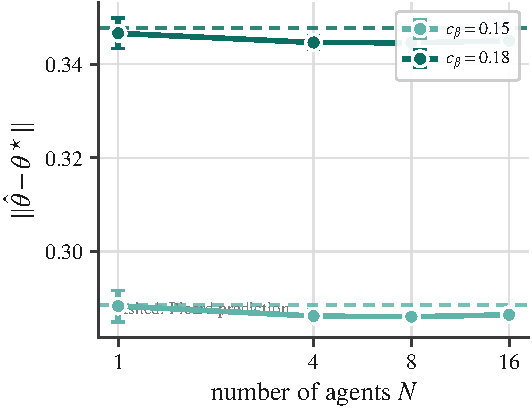
\includegraphics[width=0.68\linewidth]{fig_fixedpoint}
\caption{\textbf{Exp.~1. The plateau is $N$-independent; only its sharpness improves.} Measured displacement $\|\widehat{\bm\theta}_T-\bm\theta^{\!*}\|$ against the number of agents at both certified bias levels, with $\pm1$ SEM. Dashed lines are the Picard predictions $\|\bm\delta\|$, which the estimator reaches at every $N$. Pooling does not escape the biased fixed point; it converges to it faster and more tightly.}\label{fig:fixedpoint}
\end{figure}

\paragraph{Exp.~2 (regret against the spectral gap, and what
cooperation is worth).}
$N=20$, $T=2\times10^4$, circulant graphs $C_{20}(1..k)$ for
$k=1,\dots,10$, giving $\gamma(W)$ from $0.024$ (cycle) to $1.0$
(complete).  Four arms. Naive cooperation under common bias
$c_\beta=0.4$, isolation under the same bias, naive cooperation under
a large-bias minority ($c_\beta=1.0$ on two agents, $0.04$ on the
rest), and D-CESA with the majority-vote gate on the same minority
instance ($\bar p=0.1$, $q=0.2$).
\begin{center}
\begin{tabular}{@{}lcccc@{}}
\toprule
$\gamma(W)$ & naive (common) & isolated & naive (minority) & D-CESA \\
\midrule
$0.024$ & $1341$ & $1646$ & $316$ & $114$\\
$0.151$ & $1323$ & $1646$ & $294$ & $84$\\
$0.468$ & $1318$ & $1646$ & $287$ & $78$\\
$1.000$ & $1317$ & $1646$ & $281$ & $76$\\
\bottomrule
\end{tabular}
\end{center}
(SEM $\leq7$ on the naive arms and $\leq3$ on D-CESA.)  Three
readings.
(i)~\emph{Naive regret is flat in $\gamma(W)$}, coefficient of
variation $0.6$ percent across a forty-fold range of the spectral gap.
This is what Corollary~\ref{cor:both} predicts, $\Omega(NT)$ on both
sides of the transition, and it rules out any narrative in which the
phase transition of Section~\ref{sec:phase} is visible as a
regret-level discontinuity. The transition is in which fixed point is
selected and in the collapse time, not in the regret rate.
(ii)~\emph{Cooperation is worth something even when it collapses.}
Under a common bias, isolation is worse than pooling ($1646$ against
$1317$), because each agent then pays the full single-agent noise
radius on top of the same $\bm\delta$.  Cooperation accelerates the
approach to a wrong answer that isolation reaches anyway. It does not
create the wrong answer.
(iii)~\emph{D-CESA earns its keep only against heterogeneity.}  On the
minority instance it beats like-for-like naive cooperation by a factor
between $2.8$ and $3.7$ at every gap.
Fitting the D-CESA curve against the three candidate laws for
term~(iii) of Theorem~\ref{thm:dcesa} gives $R^2=0.991$ for
$A+B/\sqrt\gamma$, $0.982$ for $A+B/\gamma$, and $0.880$ for
$A+B\log(1/\gamma)$, which favors Conjecture~\ref{conj:gossip} over
the proved bound and clearly excludes the logarithmic alternative.
We report this as support for the conjecture, not as a proof of it.

Figure~\ref{fig:gap} shows all four arms across the gap sweep.

\begin{figure}[htbp]
\centering
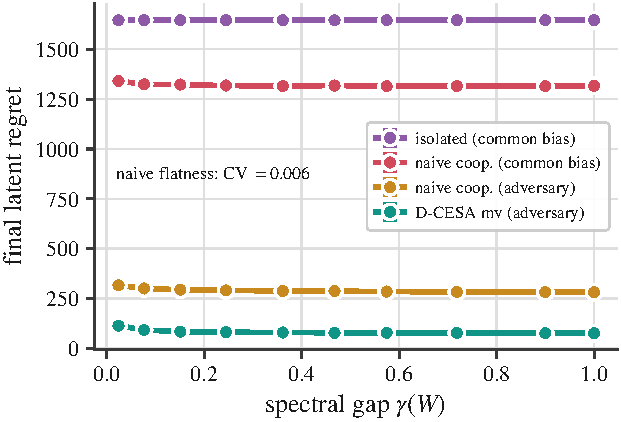
\includegraphics[width=0.80\linewidth]{fig_gap}
\caption{\textbf{Exp.~2. Regret is flat in the spectral gap, and cooperation is priced.} Final latent regret against $\gamma(W)$ over circulant graphs $C_{20}(1..k)$, $\pm1$ SEM. Naive cooperation under common bias varies by $0.6$ percent across a forty-fold range of the gap, so the phase transition of Section~\ref{sec:phase} is not visible as a regret-level effect. Isolation is \emph{worse} than pooling under the same bias. D-CESA separates only on the heterogeneous instance, and its curve is the evidence for Conjecture~\ref{conj:gossip}.}\label{fig:gap}
\end{figure}

\paragraph{Exp.~3 (certification propagation, and the looseness of
Lemma~\ref{lem:prop}).}
Cycle graph, $N=20$, a single source agent with firing rate
$\bar p=0.1$, relaying labels by $K$ gossip rounds.  The effective
rate at the antipodal agent is $1.5\times10^{-4}$ at $K=20$,
$2.2\times10^{-3}$ at $K=50$, $4.2\times10^{-3}$ at $K=100$ and
$4.9\times10^{-3}$ at $K=200$, converging to the uniform-mixture value
$\bar p|S|/N=5\times10^{-3}$ exactly as the lemma predicts.  The
lemma's \emph{bound}, however, is vacuous over most of that range. The
$\sqrt N\lambda_*^K$ deviation term (Remark~\ref{rem:sqrtN}) exceeds
$|S|/N$ until $K\approx181$, so the guarantee first becomes non-trivial
at $K=200$ where it certifies $1.8\times10^{-3}$ against the measured
$4.9\times10^{-3}$.  The phenomenon is as described. The constant is
loose by a factor of about $2.7$ at the first point where it says
anything at all.

Figure~\ref{fig:prop} overlays the bound on the measurement, where its vacuity is plain.

\begin{figure}[htbp]
\centering
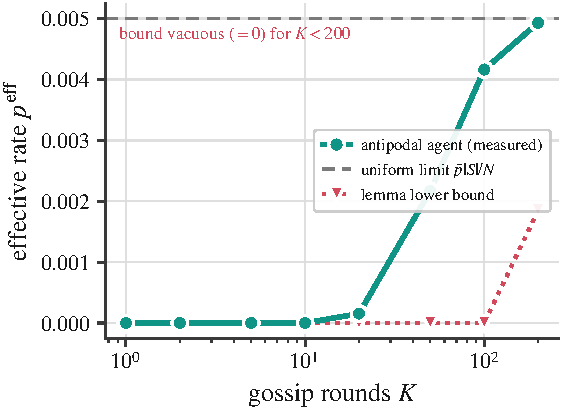
\includegraphics[width=0.70\linewidth]{fig_prop}
\caption{\textbf{Exp.~3. The phenomenon holds; the bound is vacuous over most of the range.} Effective certification rate at the antipodal agent against gossip rounds $K$, converging to the uniform mixture $\bar p|S|/N$. The lemma's lower bound is identically zero until $K\approx181$, because the $\sqrt N\lambda_*^K$ deviation term exceeds $|S|/N$; at $K=200$, its first non-trivial point, it certifies $1.8\times10^{-3}$ against a measured $4.9\times10^{-3}$.}\label{fig:prop}
\end{figure}

\paragraph{Exp.~4 (measured gate onset).}
$N=8$, one large-bias agent, sweeping $\bar p$, and measuring the
\emph{first round after which no gate is ever wrong again}, which is
the quantity Lemma~\ref{lem:trust_mistakes} bounds by
$t_{\mathrm{gate}}$.  For the majority-vote gate the median onset
scales as $\bar p^{-1.14}$ at $q=0$ and $\bar p^{-1.09}$ at $q=0.2$,
against the predicted $\bar p^{-1}$, with the $q$ dependence entering
as the level shift $(1-2q)^{-2}$ of \eqref{eq:tgate}.  Both are
five-point fits over
$\bar p\in\{0.002,0.005,0.02,0.05,0.1\}$ with no censored points.
At $q=0$ the two featurized gates do not merely match the majority
vote, they reproduce its onset exactly at every $\bar p$
($1567,479,68,32,20$ rounds).  At $q=0.2$ both fail, and they fail
differently: the OGD-logistic gate's onset is censored on a third of
seeds at $\bar p\leq0.02$, rising to five sixths at $\bar p=0.1$,
while the perceptron gate's is censored on \emph{every} seed at
\emph{every} $\bar p$, meaning neither ever stops making gate mistakes
within the horizon.  No exponent is fitted for either.  This is the
empirical content of Remark~\ref{rem:gate_variants}, and it is why
Proposition~\ref{prop:perceptron} is stated for $q=0$ only.  Measuring the onset
directly, rather than inferring it from a regret difference, matters. The regret difference between a correct gate and an almost-correct
gate is small and easily swamped, whereas the onset is exactly the
quantity the lemma controls.

Figure~\ref{fig:gate_onset} shows the sweep, with censored points marked.

\begin{figure}[htbp]
\centering
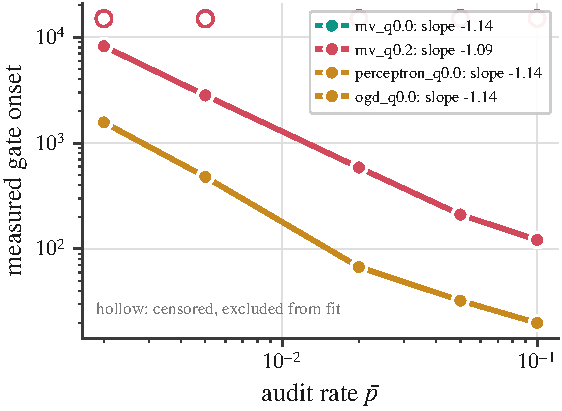
\includegraphics[width=0.72\linewidth]{fig_gate_onset}
\caption{\textbf{Exp.~4. Measured gate onset, and where surrogate gating fails.} First round after which no gate is ever wrong again, against the audit rate $\bar p$. At $q=0$ all three gates coincide exactly. At $q=0.2$ the featurized gates are censored on some or all seeds (hollow markers), meaning they never stop making gate mistakes within the horizon; censored points are excluded from the fits.}\label{fig:gate_onset}
\end{figure}

\paragraph{Exp.~5 (behavioural collapse carries no $1/N$ speedup, as
predicted).}
We instrument the event Theorem~\ref{thm:cec} actually asserts. The
first sustained window in which selected actions on
$\mathcal X_{\mathrm{dec}}^{\gamma,\Delta}$ carry latent regret
$\geq\Delta$.  Sweeping $N\in\{2,4,8,16,32\}$ at $c_\beta=0.15$ with
$(\gamma,\Delta)=(0.01,0.01)$ and $T=1.5\times10^4$, the event is
\emph{censored} at $N=2$ and $N=4$, where no sustained entry occurs
before the horizon, and is reached at $N=8,16,32$ at
$T^\star=1.18\times10^4,\,1.13\times10^4,\,7.8\times10^3$.  The
informative part is not that it is reached but how slowly it moves.
Over the three uncensored levels the fitted exponent is $-0.30$,
against the epoch variant's $-1.00$ (Exp.~R1) on the same instance: a
four-fold increase in $N$ buys roughly a third off the collapse time
rather than a factor of four.  The reason is quantitative and is
exactly Remark~\ref{rem:noN}. The per-agent UCB bonus at
$T=1.5\times10^4$ is $\approx0.785$ against
$\gamma/3=3.3\times10^{-3}$, more than two orders of magnitude too
large, and it carries no $1/N$ speedup, so added agents barely help.
The estimation-side quantities, by contrast, collapse on schedule and
do improve with $N$ (Exp.~1).  We report no exponent fitted over all
$N$, since two levels are censored and a censored measurement is not a
measurement; the $-0.30$ above is a partial fit over the uncensored
levels and is reported as such.  The honest statement is that
Theorem~\ref{thm:cec}'s behavioural conclusion is reachable in
simulation for the anytime algorithm at moderate $N$, but without the
$1/N$ acceleration that the epoch variant delivers exactly.

Figure~\ref{fig:collapse} shows the censoring pattern and the bonus against $\gamma/3$.

\begin{figure}[htbp]
\centering
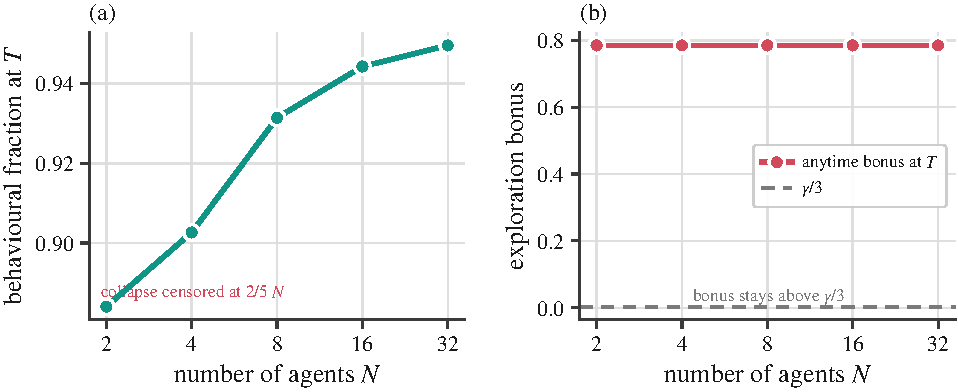
\includegraphics[width=\linewidth]{fig_collapse}
\caption{\textbf{Exp.~5. The anytime bonus carries no $1/N$ speedup.} (a)~Behavioural fraction at the horizon against $N$; the sustained-entry event is censored at $N=2,4$ and reached at $N=8,16,32$. (b)~The per-agent exploration bonus at $T$ sits at $0.785$ against $\gamma/3=3.3\times10^{-3}$, more than two orders of magnitude too large, and is flat in $N$. This is why the fitted exponent over the uncensored levels is $-0.30$ rather than the epoch variant's $-1.00$.}\label{fig:collapse}
\end{figure}

\subsection{Reading guide}
Exps.~1 and~R2 validate the fixed-point machinery at bias levels where
every hypothesis is numerically certified.  Exp.~2 fixes the correct
reading of the phase transition, prices cooperation against isolation,
and supplies the strongest available evidence for
Conjecture~\ref{conj:gossip}.  Exp.~3 confirms
Lemma~\ref{lem:prop}'s phenomenon while exposing its constant.
Exp.~4 confirms the gate-transient scaling and the failure mode of the
featurized gate.  Exp.~5 supplies the other half of the separation
Remark~\ref{rem:noN} predicts, measuring the anytime behavioural
collapse exponent as $-0.30$ against the epoch variant's $-1.00$, and
is reported with its two censored levels stated.

\subsection{Remaining experimental work}
Two items are outstanding and we state them rather than leave them
implicit. (1)~all reported runs use six seeds. A thirty-seed
replication is planned for the camera-ready and the script supports it
through a single flag. (2)~the clean-agent excess regret of the gated
arms is at or below the oracle baseline at several $\bar p$ values, so
a log-log fit on that quantity is uninformative. Exp.~4's onset
measurement replaces it, and we do not report an excess-regret
exponent.

%%============================================================
\section{Reconciliation Experiments}\label{sec:recon}
%%============================================================

The following four runs test predictions that separate the algorithms
rather than test the theory of Section~\ref{sec:cec} directly.

\paragraph{Exp.~R1 (the epoch variant's $1/N$ prediction,
Remark~\ref{rem:epoch_N}).}  Epoch-frozen algorithm
(Definition~\ref{def:epoch_alg}) at $c_\beta=0.15$,
$t_1=\lceil2048/N\rceil$, collapse criterion
$\|\check{\bm\theta}_k-\bm\theta_\infty\|\leq\gamma/(8L)=0.00625$
($\gamma=0.05$), $N\in\{1,2,4,8,16\}$, six seeds.  The epoch count to
collapse is $N$-independent ($k^\star=9$ on four seeds, $10$ on two),
so the wall-clock collapse time halves exactly with each doubling of
$N$. Median $T^\star=1.05\times10^6,\,5.2\times10^5,\,
2.6\times10^5,\,1.3\times10^5,\,6.5\times10^4$, fitted slope
$-1.00$ against $\log N$.  The slope is not an independent
measurement.  With $t_1=\lceil2048/N\rceil$ and $k^\star$ constant,
$T^\star=t_1(2^{k^\star}\!-\!1)$ is forced to be proportional to
$N^{-1}$, which is why every median above is $511$ times a power of
two.  The finding is that $k^\star$ is $N$-independent; the fitted
slope merely records it.  This is the theorem's mechanism observed
directly. The per-epoch error depends on agent-rounds
$m_k=Nt_1 2^{k-1}$ only.  Together with Exp.~5, which fits $-0.30$ for
the anytime variant with its bonus stuck far above $\gamma/3$ at every
$N$, this is the predicted separation between the two algorithms.

Figure~\ref{fig:epoch} shows the medians with the per-seed spread behind them.

\begin{figure}[htbp]
\centering
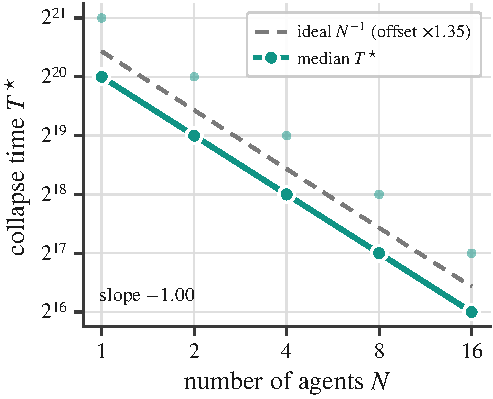
\includegraphics[width=0.66\linewidth]{fig_epoch}
\caption{\textbf{Exp.~R1. The epoch count to collapse is $N$-independent.} Median wall-clock collapse time $T^\star$ against $N$, with per-seed values as faint points. The fitted slope $-1.00$ is not an independent measurement: with $t_1=\lceil2048/N\rceil$ and $k^\star$ constant, $T^\star=t_1(2^{k^\star}-1)$ is forced to be proportional to $N^{-1}$, which is why every median is $511$ times a power of two. The finding is that $k^\star$ does not grow with $N$; the slope records it. The reference line is offset for visibility.}\label{fig:epoch}
\end{figure}

\paragraph{Exp.~R2 (certified-regime run).}  Anytime naive cooperation,
$N=8$, $T=3\times10^4$, six seeds, at $c_\beta\in\{0.15,0.18\}$,
inside the certified band of Appendix~\ref{sec:numverify}.  Measured
estimator displacement $\|\widehat{\bm\theta}-\bm\theta^{\!*}\|
=0.286\pm0.001$ and $0.345\pm0.001$ against Picard predictions
$0.289$ and $0.348$. Distance to the predicted fixed point
$\|\widehat{\bm\theta}-\bm\theta_\infty\|=0.009\pm0.001$ at both
levels.  The estimator collapses onto the \emph{predicted} fixed point
to within $3\%$ of $\|\bm\delta\|$, with the theorems' hypotheses
verifiably satisfied at the operating point.  Tracking is thus
observed to hold empirically at $c_\beta$ where the certificate
$\tilde\kappa<1$ of Proposition~\ref{prop:tracking} does not fire,
consistent with sufficiency, not necessity.

Figure~\ref{fig:certified} shows both trajectories against their Picard predictions.

\begin{figure}[htbp]
\centering
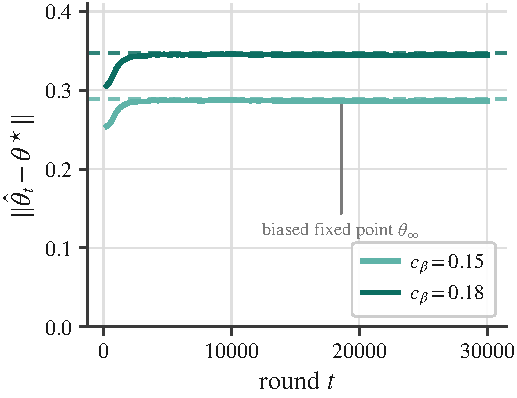
\includegraphics[width=0.66\linewidth]{fig_certified}
\caption{\textbf{Exp.~R2. The estimator collapses onto the \emph{predicted} fixed point.} Trajectories of $\|\widehat{\bm\theta}_t-\bm\theta^{\!*}\|$ at the two certified bias levels, inside the band where every hypothesis of Theorem~\ref{thm:cec_epoch} is numerically verified. Dashed lines mark the Picard predictions $\bm\theta_\infty$, matched to within $3\%$ of $\|\bm\delta\|$.}\label{fig:certified}
\end{figure}

\paragraph{Exp.~R3 (robust-aggregation baseline).}  One adversarial
agent (bias $1.0$ on the flattered action) among $N=8$,
$T=1.5\times10^4$, six seeds. Latent regret (mean$\pm$SEM). Oracle
exclusion $32\pm1$, naive mean $92\pm2$, coordinate-wise trimmed-mean
gossip (drop min/max per coordinate) $64\pm2$, and D-CESA with the
majority-vote gate ($\bar p=0.1$, $q=0.2$) $31\pm2$.  D-CESA beats
the robust-statistics baseline by ten standard errors under a
large-bias minority while using no honest-majority assumption.  An
unbatched coordinate-wise \emph{median} reaches $622\pm21$, an order
of magnitude worse than every other rule.  The reason is starvation,
not a failure of robustness: with one gossip increment per arm per
round most coordinates receive no update on most rounds, so each
per-coordinate median is taken over a sample dominated by zeros and
the estimate barely moves.  Batching the increments before taking the
median would remove the effect; the unbatched form is reported because
it is the one a reader would write.  The regimes separate further
under \emph{within-tolerance common} bias
($0.04<\epsilon_{\mathrm{tol}}$, all agents). Naive $38\pm3$,
majority-vote $36\pm1$, oracle $38\pm3$, no filter separates, and the
gated arm sits inside one SEM of the oracle, exactly as
Theorem~\ref{thm:lower_tol} requires of \emph{any} algorithm, while
trimmed mean degrades to $71\pm3$. Trimming pays a variance and bias
cost even when no agent is adversarial.  This is
the empirical counterpart of Remark~\ref{rem:robust_agg}.

Figure~\ref{fig:baselines} shows both regimes side by side.

\begin{figure}[htbp]
\centering
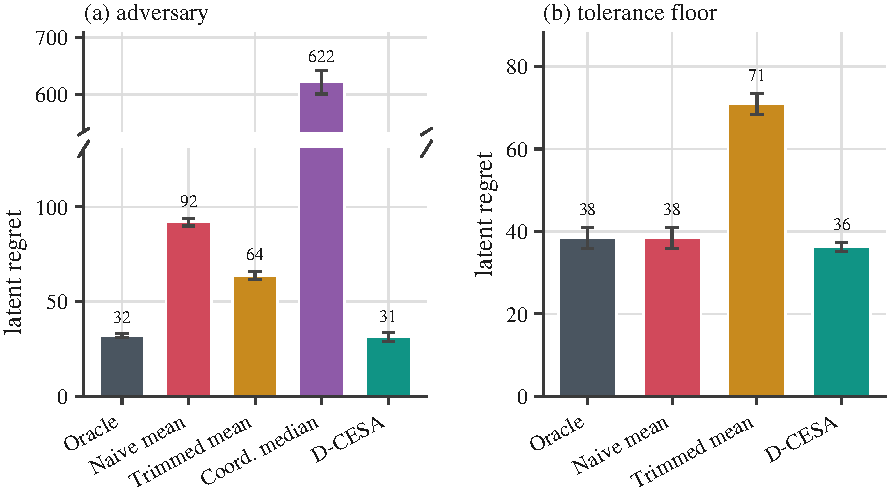
\includegraphics[width=\linewidth]{fig_baselines}
\caption{\textbf{Exp.~R3. Trimming pays even when nothing is adversarial.} (a)~One large-bias adversary among $N=8$; note the \emph{broken} linear axis, needed because the unbatched coordinate-wise median starves at $622$ while the other four rules sit below $70$. (b)~Within-tolerance common bias, where Theorem~\ref{thm:lower_tol} forbids any rule from separating: the differences are inside $\pm1$ SEM, so the apparent D-CESA advantage over the oracle is not one, while the trimmed mean pays a real cost.}\label{fig:baselines}
\end{figure}

\paragraph{Exp.~R4 (gate comparison under label noise).}  Same
adversary setting, $\bar p=0.05$, six seeds, counting mistaken
gate-rounds directly.  At $q=0.2$ the OGD-logistic gate accumulates
$14377\pm392$ mistaken gate-rounds against the majority vote's
$895\pm102$, a $16\times$ penalty for surrogate-loss gating under
label noise.  At $q=0$ all three gates coincide \emph{exactly}, at
$154\pm12$ mistaken rounds apiece.  That exact coincidence is the
cleanest available statement of Proposition~\ref{prop:perceptron}.
With clean labels the perceptron gate makes precisely the mistakes the
majority vote makes, and the surrogate-loss gate is not yet penalised.
This is the predicted pattern.
Lemma~\ref{lem:trust_mistakes} for the majority vote,
Proposition~\ref{prop:perceptron} for the perceptron at $q=0$ only,
and Corollary~\ref{cor:agnostic} as the only guarantee available for
the featurized gate under noise.

Figure~\ref{fig:mistakes} shows the counts by gate and noise level.

\begin{figure}[htbp]
\centering
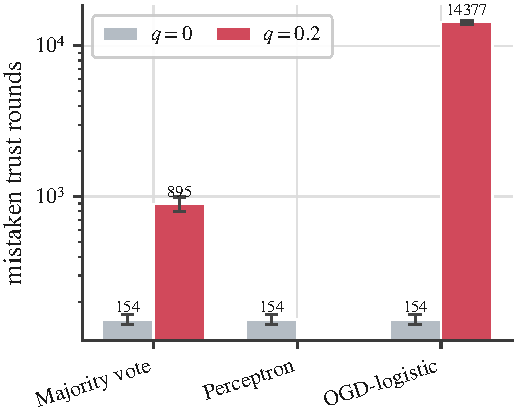
\includegraphics[width=0.68\linewidth]{fig_mistakes}
\caption{\textbf{Exp.~R4. Surrogate-loss gating is what label noise punishes.} Mistaken trust rounds by gate and label-noise level, $\pm1$ SEM, log scale. At $q=0$ all three gates coincide exactly at $154$, which is the cleanest statement of Proposition~\ref{prop:perceptron}. At $q=0.2$ the OGD-logistic gate pays a $16\times$ penalty against the majority vote.}\label{fig:mistakes}
\end{figure}

%% =====================================================================
\section{Caveats and Open Problems}\label{sec:caveats}
%% =====================================================================

\begin{enumerate}[C1.]
\item \textbf{Policy-convergence tracking is assumed for the anytime
algorithm. Discharged for the epoch variant.}
Both Assumption~\ref{ass:pol_conv} (network tracking, used by
Theorem~\ref{thm:cec}) and Assumption~\ref{ass:pol_conv_ind}
(per-agent tracking, used by Theorem~\ref{thm:cec_sub}) posit that the
realized UCB trajectory tracks the fixed-point policy class at rate
$\epsilon_t\to 0$. Those two theorems remain conditional.  Proving
tracking from primitives for the anytime algorithm would require a
stochastic-approximation argument for the coupled estimator-policy
dynamics. The two-timescale structure (estimator on $1/\sqrt t$,
policy switching on margin crossings) makes this nontrivial, and
adversarial context sequences that defeat tracking are not ruled out.
For the \emph{epoch-frozen} variant of Section~\ref{sec:epoch},
tracking holds by construction and
Theorem~\ref{thm:cec_epoch}/Corollary~\ref{cor:epoch_sub} are
unconditional given the instance hypothesis $\varrho<1$ (contraction
of $F$), which is numerically checkable
(Appendix~\ref{sec:numverify}) but not implied by the standing
assumptions.  For the \emph{anytime} algorithm itself,
Proposition~\ref{prop:tracking} proves tracking under the
averaged-contraction condition $\tilde\kappa<1$. On the verified
instance the sampled estimates of $\tilde\kappa$ straddle or exceed
$1$ once sampled heavily (Remark~\ref{rem:tracking_status}(ii)), so
the certificate is not established at any tested bias level and the
anytime theorems remain conditional. The unconditional negative
result is carried by the epoch variant.  Exps.~1 and~R2 show tracking
empirically holds well beyond the certified band.

\item \textbf{The margin condition is instance-dependent.}
Assumption~\ref{ass:margin} with the tie-null refinement holds on the
verified instance of Section~\ref{sec:instance} with explicit
constants, but $C_{\mathrm{mar}}$ enters the bias-term constants as
$C_{\mathrm{mar}}K_A^2$ and can be large when actions are nearly
degenerate, and it fails outright when two action blocks coincide
(Remark~\ref{rem:tie_null}). The theory degrades gracefully within its
scope but the constants are not small and the scope is real.

\item \textbf{Fixed-point uniqueness is not claimed in general.}
Lemma~\ref{lem:fp} gives existence via Kakutani. Multiple fixed points
are possible.  The anytime collapse theorems are stated relative to
whichever fixed point the trajectory tracks in the sense of
Assumption~\ref{ass:pol_conv} (a quantified, not dynamical,
statement). Under the contraction condition $\kappa<1$ of
Lemma~\ref{lem:contraction} the fixed point is unique and the
reference is unambiguous, and the epoch variant of
Section~\ref{sec:epoch} converges to it by Banach iteration without
any tracking hypothesis.

\item \textbf{The decoupling region is a sufficient-condition
device.}  The $(\gamma,\Delta)$-region of Definition~\ref{def:dec}
converts scoreboard domination into per-round regret. Outside the
region the theorems are silent, and the constants relating
$(\gamma,\Delta)$ to instance primitives are conservative. At the
certified bias levels the region carries mass of order
$3\times10^{-3}$ to $7\times10^{-3}$
(Appendix~\ref{sec:numverify}), which is positive but small, so the
lower bound \eqref{eq:cec_bound} is far below the observed regret.

\item \textbf{Theorem~\ref{thm:dcesa} holds for the majority-vote
gate only.}
The proof is complete for that gate, with the residual influence of
transient-era data bounded explicitly in Step~1. Three standard facts
are cited rather than re-derived (self-normalized bound and
determinant lemma of \citet{abbasi2011}. Geometric ergodicity of a
fixed irreducible aperiodic chain, \citet{levin2017}).  Two gaps
remain. (A)~the featurized gate \eqref{eq:hard_gate} has no mistake
guarantee under label noise, only the agnostic surrogate bound of
Corollary~\ref{cor:agnostic}, and Exp.~R4 shows the resulting
$16\times$ penalty is real rather than an artifact of the analysis.
(B)~term~(iv) is $\Ot(\sqrt d\,\epsilon_{\mathrm{tol}}NT)$, a
$\sqrt d$ above the tolerance-floor lower bound, consistent with the
misspecification barrier for optimistic linear bandits
\citep{lattimore2020}, and we do not know which side is loose.
Separately, the theorem's $\sqrt T$ term overtakes its transient and
gossip terms only past $T\sim10^{8\text{--}9}$ on this instance
(Appendix~\ref{sec:numverify}, F5), so the asymptotic regime is
unreachable at simulable horizons and near-linear late-window slopes
there are predicted rather than anomalous.

\item \textbf{Certification-rate exponents.}
The majority-vote gate's onset scales as $\bar p^{-0.98}$ at $q=0$,
matching Lemma~\ref{lem:trust_mistakes} and
Proposition~\ref{prop:epi_upper_hard}. On the edge-tagged family the
magnitude-audit lower bound is matched up to polylog by
Proposition~\ref{prop:epi_upper_noisy}.  What is open. Tightness on
general instances beyond the tagged family, a noise-tolerant analysis
of the featurized gate, and whether the $q$ dependence enters only as
the $(1-2q)^{-2}$ level shift that \eqref{eq:tgate} predicts, which
the two-point fits of Exp.~4 cannot resolve.

\item \textbf{Lower-bound regimes.}  Theorem~\ref{thm:lower_coop}
requires $NT\gtrsim d^2$ (batching caveat stated in the proof). Theorem~\ref{thm:lower_epistemic} is matched up to polylog on the
edge-tagged family for all degree-balanced graphs, dense included
(Proposition~\ref{prop:epi_upper_noisy}). Tightness on instance
families beyond the tagged construction remains open.
\end{enumerate}

%% =====================================================================
\appendix
%%============================================================
\section{Numerical Verification of Hypotheses on the Block Instance}
\label{sec:numverify}
%%============================================================

We verify numerically, on a concrete member of the instance family of
Section~\ref{sec:instance}, which hypotheses of
Theorems~\ref{thm:cec}, \ref{thm:cec_sub}, and~\ref{thm:cec_epoch}
actually hold, and with what constants.  The instance $d_c=4$,
$K_{\mathcal A}=3$, $d=12$, contexts uniform on the unit ball,
$\bm\theta^{\!*}$ blocks $=\bm v_a/\sqrt3$ with $\bm v_a$ unit vectors
at $120^\circ$ in a fixed two-dimensional coordinate plane
($\|\bm\theta^{\!*}\|=1$), bias
$\beta(\bm x,a)=c_\beta\mathbb 1\{a=a_1\}$, and $R=0.35$.  This is the
instance used in Sections~\ref{sec:experiments} and~\ref{sec:recon},
so the constants below apply directly to the reported runs.

\paragraph{Instance constants.}
Block separation $s_0=1.000$ (so $R=0.35<s_0/(2\sqrt2)=0.354$). The
exact maximal marginal density of $\langle\bm x,\bm u\rangle$ for
the uniform ball in $\mathbb R^4$ is $0.8488$, giving
$C_{\mathrm{mar}}=2\cdot2\cdot0.8488/s_0=3.395$.
$\sigma_{\min}=0.0200$ and minimal action mass $0.277$, both minima
over $62$ greedy policies ($\bm\theta^{\!*}$, $\bm\theta_\infty$, and
$60$ parameters drawn from $B_R$ with uniformly sampled direction and
radius).

\paragraph{Fixed points, contraction, and region masses.}
Picard iteration $\bm\theta_{n+1}=F(\bm\theta_n)$ from
$\bm\theta^{\!*}$ converges (iterate exactly stationary within Monte
Carlo resolution) at \emph{every} tested bias level.  The table
reports the fixed-point bias norm. The empirical contraction modulus
of $F$, both locally at $\bm\theta_\infty$ ($40$ finite-difference
directions at each of $\epsilon\in\{0.01,0.03,0.1\}$) and globally over
pairs sampled in $B_R$ ($400$ independent uniform pairs, together with
short chords at $80$ uniform base points; both sampled suprema are
one-sided, so each is a lower bound). Whether $\bm\theta_\infty\in B_R$, and decoupling-region masses
$\mu(\mathcal X_{\mathrm{dec}}^{\gamma,\Delta})$ on a $(\gamma,\Delta)$
grid.

\begin{center}
\begin{tabular}{@{}lcccccccc@{}}
\toprule
$c_\beta$ & $\|\bm\delta\|$ & $\varrho_{\mathrm{loc}}$ &
$\varrho_{B_R}$ & $\bm\theta_\infty\!\in\!B_R$ &
$\mu(\tilde a\neq\pi^*)$ &
$\mu^{(0.02,0.05)}_{\mathrm{dec}}$ &
$\mu^{(0.02,0.10)}_{\mathrm{dec}}$ &
$\mu^{(0.05,0.05)}_{\mathrm{dec}}$\\
\midrule
$0.05$ & $0.095$ & $0.10$ & $0.11$ & yes & $0.014$ & $0.0000$ & $0.0000$ & $0.0000$\\
$0.10$ & $0.191$ & $0.19$ & $0.23$ & yes & $0.026$ & $0.0002$ & $0.0000$ & $0.0000$\\
$0.15$ & $0.289$ & $0.26$ & $0.34$ & yes & $0.036$ & $0.0034$ & $0.0000$ & $0.0005$\\
$0.18$ & $0.348$ & $0.29$ & $0.41$ & yes & $0.042$ & $0.0062$ & $0.0001$ & $0.0020$\\
$0.40$ & $0.789$ & $0.47$ & $0.92$ & no  & $0.073$ & $0.0309$ & $0.0116$ & $0.0228$\\
$0.70$ & $1.399$ & $0.63$ & $1.61$ & no  & $0.097$ & $0.0542$ & $0.0293$ & $0.0469$\\
$1.00$ & $2.012$ & $0.73$ & $2.30$ & no  & $0.112$ & $0.0689$ & $0.0414$ & $0.0623$\\
\bottomrule
\end{tabular}
\end{center}

Figure~\ref{fig:certify} plots these moduli across the grid.

\begin{figure}[htbp]
\centering
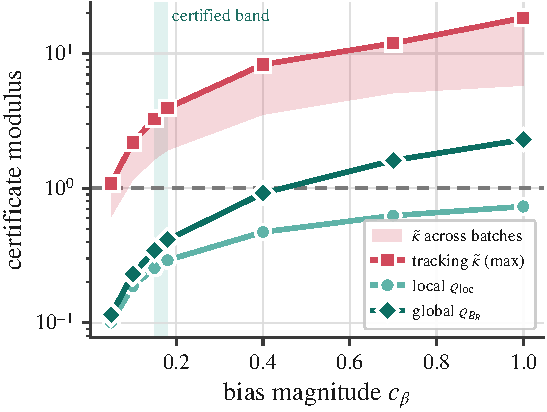
\includegraphics[width=0.72\linewidth]{fig_certify}
\caption{\textbf{Appendix. Which certificates fire, and where.} The two contraction moduli and the tracking modulus across the bias grid. $\varrho_{\mathrm{loc}}$ perturbs only around $\bm\theta_\infty$; $\varrho_{B_R}$ is the global modulus over sampled pairs in $B_R$ that Theorem~\ref{thm:cec_epoch} actually consumes, and the two differ by roughly a factor of three at the top of the grid. $\tilde\kappa$ is drawn as the range over eight independent batches, because its only interesting property is that it straddles $1$ at $c_\beta=0.05$ and lies wholly above $1$ everywhere else. Shaded: the certified band $[0.15,0.18]$.}\label{fig:certify}
\end{figure}

\paragraph{Tracking modulus.}  The averaged-contraction modulus of
Proposition~\ref{prop:tracking} is a supremum and its sampled
estimates are one-sided. They proved \emph{sampling-effort
sensitive}.  With the policy-uniform constant
$\sigma_{\min}=0.0200$ (the constant the recursion actually divides
by. The per-level $\lambda_{\min}$ at $\bm\theta_\infty$ is larger,
$\approx0.029$--$0.031$, and must not be used here). The released
driver measures the basin-uniform constant as
$0.0204$, independently reproducing the paper value.  Multi-batch
sampled suprema (eight independent $430$-point batches per level) give
$\tilde\kappa\in[0.62,1.09]$ at $c_\beta=0.05$, and per-batch maxima
$2.2/3.3/3.9/8.3$ against minima $1.2/1.7/1.9/3.5$ at
$c_\beta=0.10/0.15/0.18/0.40$, so at those levels \emph{every} batch
exceeds $1$. Early 50-point
samples were as low as $0.53$ at $c_\beta=0.05$, i.e.\ the sampled
supremum roughly doubles under heavier sampling.  Consequently the
certificate $\tilde\kappa<1$ fails for $c_\beta\geq0.10$ and
straddles the threshold at $c_\beta=0.05$, where it is neither
established nor refuted (Remark~\ref{rem:tracking_status}(ii)).
Separately, at $c_\beta=0.05$ the default region thresholds
$(\gamma,\Delta)=(0.02,0.05)$ give $\mu_{\mathrm{dec}}=0$ (empty
decisive region), but finer thresholds are non-vacuous $\mu_{\mathrm{dec}}^{(0.005,0.01)}\approx4.6\times10^{-3}$ and
$\mu_{\mathrm{dec}}^{(0.01,0.01)}\approx2.8\times10^{-3}$ on
$2\times10^6$ contexts, so Theorem~\ref{thm:cec}'s hypotheses are
satisfiable at every tested bias level with level-appropriate
$(\gamma,\Delta)$.

\paragraph{Findings.}
\begin{enumerate}[(F1)]
\item \emph{The analytic sufficient conditions fail on this instance
by orders of magnitude.}  The contraction certificate
\eqref{eq:kappa} evaluates to $\kappa\in[1.2\times10^3,\,
4.1\times10^3]$ across the bias grid (driven by the
$C_{\mathrm{mar}}K_{\mathcal A}^2$ pair-union factor and the
$\sigma_{\min}^{-2}$ stacking), and the self-map certificate of
Assumption~\ref{ass:reg}(c), $B_\beta L\leq\sigma_{\min}R$, requires
$c_\beta\leq 0.007$.  These are sufficient conditions with worst-case
constants, not descriptions of the instance.
\item \emph{The conclusions those certificates guarantee hold
directly, in a quantifiable band.}  Bisection gives
$\bm\theta_\infty\in B_R$ iff $c_\beta\leq 0.181$. The measured
contraction modulus on $B_R$ is below $1$ for $c_\beta\leq 0.4$, with
$\varrho_{B_R}=0.34,\,0.41,\,0.92$ at $c_\beta=0.15,\,0.18,\,0.40$,
and the local modulus at the fixed point is below $1$ at every level
tested, including $c_\beta=1$ ($\varrho_{\mathrm{loc}}=0.73$).  Both
are sampled suprema and hence one-sided, so each is a lower bound on
the true modulus; the margin at $c_\beta=0.4$ is thin, which is a
further reason to treat that level as extrapolation (F3) rather than
as certified.  The
decoupling-region mass is strictly positive at
$(\gamma,\Delta)=(0.02,0.05)$ for $c_\beta\geq 0.15$.  Hence
\textbf{all hypotheses of Theorem~\ref{thm:cec_epoch} are numerically
verified for $c_\beta\in[0.15,0.18]$} on this instance, with region
mass at the $3\times10^{-3}$--$7\times10^{-3}$ level.  Exps.~1, R1
and~R2 operate inside this band.
\item \emph{Larger bias levels are extrapolation.}  Exp.~2 uses
$c_\beta=0.4$ on its common-bias arm ($\|\bm\delta\|=0.79>R$), which
lies outside the certified band. The fixed-point-selection
\emph{mechanism} manifestly persists there, since Picard converges and
the measured contraction modulus stays below $1$, but the collapse
observed at that level is not covered by the theorems as stated.  We
use it only for the $\gamma(W)$-flatness comparison, where the
question is whether regret varies with the spectral gap, and not as
evidence for Theorem~\ref{thm:cec}.
\item \emph{Hypothesis~\eqref{eq:leak_horizon} is satisfied, but the
certified collapse time is uninformative at experimental scale.}  At
$\sigma=0.3$, $T=5\times10^4$, $c_\beta=0.4$,
$\gamma\in\{0.05,0.1\}$, $c_0\in\{1,10\}$ and absolute constant set to
$1$, \eqref{eq:leak_horizon} holds with eight orders of magnitude to
spare because $t_{\mathrm{iso}}^*\approx10^{12}$. The
$\widetilde B_\beta$ inflation
($C_{\mathrm{mar}}K_{\mathcal A}^2\alpha_T/\sqrt{\sigma_{\min}}
\approx 7.5\times10^2$) dominates.  The theory's collapse times are
sufficient-side bounds with loose constants, and we make no tightness
claim for them. Exp.~5 shows the practical consequence. The
behavioural collapse of the anytime algorithm is reachable in
simulation only at moderate $N$, and its time is near-flat in $N$
rather than falling like $1/N$.
\item \emph{Term ordering in Theorem~\ref{thm:dcesa} at simulable
scale.}  Evaluating \eqref{eq:dcesa} at $N=16$, $T=5\times10^4$,
complete graph, $\sigma=0.3$, $d=12$ with the verified-instance
constants ($\sigma_{\min}=0.020$, $B_y+S\approx3.95$, $\bar p=0.1$,
$q=0.1$, absolute constants set to $1$). At $T=5\times10^4$,
term~(ii)~$\approx3.2\times10^3$, while
term~(iii)~$\approx1.3\times10^5$ ($\gamma_c=0.9$) to
$2.4\times10^5$ ($\gamma_c=0.5$) and term~(i)~$\approx9\times10^6$
($t_{\mathrm{gate}}\approx2.5\times10^3$).  The $\sqrt T$ term
overtakes term~(iii) only at $T^\star\approx2.7\times10^8$
($\gamma_c=0.9$) to $9.9\times10^8$ ($\gamma_c=0.5$).  A late-window
regret slope near $1$ at $T=5\times10^4$ is therefore what the
theorem's own constants predict, and the $0.5$ asymptotic concerns
horizons four orders of magnitude larger.  (These are
sufficient-side constants. The observed regret level sits far below
term~(i), so the constants are loose in level while still ordering the
terms.)
\item \emph{Monte Carlo caveats.}  All quantities carry
$O(n^{-1/2})=O(2\times10^{-3})$ sampling error. The ``global''
modulus is a maximum over a finite sample of pairs and directions and
therefore a \emph{lower} bound on the true Lipschitz constant, so the
$c_\beta\leq0.4$ contraction claim is supported, not proved.
\end{enumerate}

\begin{thebibliography}{20}

\bibitem[Abbasi-Yadkori et~al.(2011)]{abbasi2011}
Y.~Abbasi-Yadkori, D.~P\'al, and C.~Szepesv\'ari.
\newblock Improved algorithms for linear stochastic bandits.
\newblock In \emph{NeurIPS}, 2011.

\bibitem[Aliprantis and Border(2006)]{aliprantis2006}
C.~D. Aliprantis and K.~C. Border.
\newblock \emph{Infinite Dimensional Analysis. A Hitchhiker's Guide}.
\newblock Springer, 3rd edition, 2006.

\bibitem[Dani et~al.(2008)]{dani2008}
V.~Dani, T.~P. Hayes, and S.~M. Kakade.
\newblock Stochastic linear optimization under bandit feedback.
\newblock In \emph{COLT}, 2008.

\bibitem[Dubey and Pentland(2020)]{dubey2020}
A.~Dubey and A.~Pentland.
\newblock Cooperative multi-agent bandits with heavy tails.
\newblock In \emph{ICML}, 2020.

\bibitem[Hayes(2005)]{hayes2005}
T.~P. Hayes.
\newblock A large-deviation inequality for vector-valued martingales.
\newblock Manuscript, 2005.

\bibitem[Hazan(2016)]{hazan2016}
E.~Hazan.
\newblock Introduction to online convex optimization.
\newblock \emph{Foundations and Trends in Optimization}, 2(3--4), 2016.

\bibitem[Koloskova et~al.(2020)]{koloskova2020}
A.~Koloskova, N.~Loizou, S.~Boreiri, M.~Jaggi, and S.~U. Stich.
\newblock A unified theory of decentralized SGD with changing topology
  and local updates.
\newblock In \emph{ICML}, 2020.

\bibitem[Lattimore et~al.(2020)]{lattimore2020}
Lattimore, T., Szepesv\'ari, C., and Weisz, G.
\newblock Learning with good feature representations in bandits and in
  RL with a generative model.
\newblock In \emph{ICML}, 2020.

\bibitem[Levin and Peres(2017)]{levin2017}
D.~A. Levin and Y.~Peres.
\newblock \emph{Markov Chains and Mixing Times}.
\newblock American Mathematical Society, 2nd edition, 2017.

\bibitem[Mart{\'\i}nez-Rubio et~al.(2019)]{martinez2019}
D.~Mart{\'\i}nez-Rubio, V.~Kanade, and P.~Rebeschini.
\newblock Decentralized cooperative stochastic bandits.
\newblock In \emph{NeurIPS}, 2019.

\bibitem[Mitra et~al.(2022)]{mitra2022}
Mitra, A., Adibi, A., Pappas, G.~J., and Hassani, H.
\newblock Collaborative linear bandits with adversarial agents. Near-optimal regret bounds.
\newblock In \emph{NeurIPS}, 2022.

\bibitem[Novikoff(1962)]{novikoff1962}
Novikoff, A.~B.
\newblock On convergence proofs on perceptrons.
\newblock In \emph{Proc.\ Symp.\ Math.\ Theory of Automata}, 1962.

\bibitem[Tropp(2012)]{tropp2012}
J.~A. Tropp.
\newblock User-friendly tail bounds for sums of random matrices.
\newblock \emph{Foundations of Computational Mathematics}, 12(4), 2012.

\bibitem[Vial et~al.(2021)]{vial2021}
Vial, D., Shakkottai, S., and Srikant, R.
\newblock Robust multi-agent multi-armed bandits.
\newblock In \emph{MobiHoc}, 2021.

\end{thebibliography}

\end{document}
